\documentclass{report}
\usepackage[a4paper, total={17cm, 24cm}]{geometry}
\usepackage{amsmath}

\usepackage{hhline}
\usepackage{bm}
\usepackage{pgfplots}
\usepackage{amssymb}
\usepackage{algorithm}
\usepackage{algorithmicx}
\usepackage{algpseudocode}
\usepackage{color, soul}
\usepackage[backend=biber]{biblatex}
\addbibresource{references.bib}
\graphicspath{{images/}}


%opening
\title{Honours Thesis}
\author{Ash}

\def\BState{\State\hskip-\ALG@thistlm}

\newcommand{\TODO}[1]{\sethlcolor{pink}\hl{\\(#1)\\}}
\newcommand{\FEEDBACK}[1]{\sethlcolor{green}\hl{\\ Feedback: \\#1\\}}
\newcommand{\TOCITE}[2][citation needed]{\textsuperscript{\underline{#1}}}
\newcommand\ddfrac[2]{\frac{\displaystyle #1}{\displaystyle #2}}


\begin{document}

%%	\maketitle
\begin{titlepage}
 \begin{center}
  \vspace*{5cm}
  {\huge \textbf{Honours Thesis}} \\
  \vspace{0.3cm}
  {\large Few-Shot Continuous Meta-Learning with Neural Networks} \\
  \vspace*{2cm}
  \textbf{Author} \\
  \textit{Ash Hall} \\
  Honours Student \\
  Department of Computer Science \\
  La Trobe University \\
  \vspace{0.75cm}

  \textbf{Supervisor} \\
  \textit{Zhen He} \\
  Professor \\
  Department of Computer Science \\
  La Trobe University \\


  \vfill
 \end{center}
\end{titlepage}

\chapter*{Acknowledgements}
\thispagestyle{empty}
I would like to thank Aiden, Brandon and Zhen for their guidance and advice throughout this study. It would have been a much more difficult task without their assistance!

\clearpage


\thispagestyle{empty}
\newpage
\thispagestyle{empty}
\tableofcontents
\newpage
\thispagestyle{empty}
\listoffigures
\newpage

\chapter{Introduction}
Computer vision is the task of endowing a computer system with some level of intelligence pertaining to image data. This diverse field covers as broad topics as video tracking, pose estimation, and image restoration; however for this proposal we will consider the task of image classification -- predicting the category of object in an image. \par
While the interpretation of visual stimuli is considered a simple task for living things, the equivalent is of great difficulty for a computer system. Much progress has been made since the advent of artificial intelligence for computer vision in the 1960s, with techniques evolving from human-engineered solutions to data-driven learning algorithms. The most significant development in recent times is that of neural networks -- machine learning systems that loosely emulate the behaviour of the biological brain. \par
Recently, \emph{deep learning} algorithms -- neural networks comprising of many layers of connections -- have had profound success in computer vision tasks, yet a consistent detriment to data-driven systems is that they typically require large volumes of training data in order to adequately learn. Having a system learn from few examples is crucial to building systems viable for real-world scenarios, as the acquisition of large datasets is typically difficult and expensive, making it a prohibitive factor in many cases. In addition to this, the continual usage of neural networks has been fairly restricted due to their inherent incapacity to easily learn new tasks incrementally. A typical neural network trained to predict $n$ classes cannot generalise to an additional class without retraining the entire classifier on all $n+1$ classes. This is due to the phenomenon of catastrophic forgetting. \par
Although neural networks were heavily inspired by the functioning of the biological brain, a critical difference is that humans learn tasks rapidly after only a few examples, and don't forget old knowledge to make way for new. The limitations of requiring large amounts of data and rapidly forgetting are yet to be resolved, but are a crucial step towards the widespread usage of artificial intelligence. These two limitations have resulted in a notable amount of attention being given to \emph{few-shot learning}\parencite{maml}\parencite{relationnet} -- learning a new task having seen very few examples; and  \emph{continuous learning}\parencite{lwf}\parencite{ewc}\parencite{hat} -- continuously teaching an artificial intelligence with additional knowledge over time. These have led to the exploration of \emph{meta learning}\parencite{lotsag}\parencite{maml}\parencite{reptile}\parencite{mlwtc}, which is the application of machine learning algorithms to not just learning a task but to the learning \emph{procedure}, hence learning the learning algorithm itself. This technique -- also known as \emph{learning to learn} -- has shown great potential, and has had particular success in few-shot learning\parencite{maml}\parencite{matching}\parencite{mlwtc}. \par

No research thus far has successfully merged these two tasks to result in a practicable, usable continuous learning system that only requires a few examples to continue learning throughout its life. We bridge this gap, and present a system that allows for the augmentation of an image classification neural network, where showing only a handful of images from a new collection of classes allows the model to sufficiently learn to classify both the new classes, and previously learnt classes. We do this by taking a pre-trained image classification neural network and presenting it some new images; an external neural network monitors this process and produces a new model. \par

The task is an inherently difficult one, combining two currently unsolved tasks to form a more challenging set of requirements. Continuous learning focuses on the retention of knowledge already present in a set of weights, whereas few-shot learning typically focuses on models that are capable of rapid change. These tasks appear to have contradicting properties, thereby making their overlap rather complex in its nature. Typical gradient-descent neural network algorithms don't succeed at this task due to their inability to retain information or to rapidly re-parametrise a model. \par

We present a meta learning system which exposes a small number of examples from a new set of classes to an existing classifier to compute gradients. These gradients, along with their corresponding weights are given as input to the Meta-Learner, which produces a set of optimal weight-updates as its outputs. The produced model is capable of adequately performing classification across both the original classes as well as those newly-presented. \par

Our solution is $\sim$3x as effective at adapting to new classes from few examples as a naive implementation, and also largely retains original classification performance. The Meta-Learner is capable of producing a model which performs 10\% better on the new classes than on those that it was originally trained on, indicating that it learns a dramatically improved optimisation technique over standard gradient-descent methods. We also introduce a measure of model prediction bias by the name of Batch Prediction Entropy, useful as a diagnostic tool during training. \par


We begin in chapter \ref{background:1} with an introduction to computer vision in general, before progressing to more modern and relevant information pertaining to this proposal. In chapter \ref{related:1} we will discuss works related to this task -- and those that could be considered a source of inspiration -- and will consider the benefits and detriments of each. In chapter \ref{problem-definition} we formalise our objective, define some metrics and perform some preliminary investigation. In chapter \ref{methodology} we describe our solution methodology and implementation, followed by our experimental setup in chapter \ref{experimental-setup}. Finally, we explore and discuss our results in chapter \ref{results-chapter} and finish with a conclusion and overview of our algorithm. \par

\chapter{Background} \label{background:1}
Images are sources of highly-dimensional data for which humans have the incredible ability of understanding. Developing computer vision systems that perform to even a similar capacity to that of humans is an inherently difficult task. The gift of easily converting pixel values into meaningful concepts is a skill that computer vision experts have been attempting to transfer to computers for decades. \par
The ability to quickly gain an understanding of a new concept is a uniquely human trait. Consider that after seeing a zebra only once, most humans would be able to easily identify it in a humorous police line-up  -- perhaps after the theft of a monkey's balloon --  but the best image recognition systems over the years would be dependant on seeing many examples of zebras. It is quite standard to present hundreds of examples of each new concept in order to learn which parts of the image data are unimportant noise, and which parts are characteristic of the class the image belongs to. \par
Modern techniques have made great advances in the application of meta-learning techniques (learning to learn) to few-shot learning; the task of having a computer vision system learn to recognize images from only a few labelled examples. Meta-learning has also been applied to continuous learning, and while the results have been very encouraging, the problem of catastrophic forgetting persists. The challenge of continuous learning is to teach new classes to a system without interfering with the previously learnt tasks. \par
We will now explore neural-networks more thoroughly, and how advancements in the field have put us in a good position to tackle few-shot and continuous learning. First we will discuss the motivations for data-driven machine learning, the breadth of applicable tasks, and how these can be achieved. We will end with the problems regularly encountered with small datasets and how modern architectures seek to resolve these. \par

\section{Hand Engineered and Learnt Features} \label{hand-eng:1}
Features are a general term for characteristic attributes which exist across all samples in a dataset or domain. These features were traditionally hand-engineered by machine learning experts, carefully selecting the base-components of which the dataset in question appears to comprise. A common hand-engineered feature is the Histogram of Oriented Gradients (fig \ref{fig:hog:1}), which results in small regions of an image voting on the best description of the local gradient. \par
However, a fundamental problem with hand-engineered features is that it imposes human knowledge onto a problem to be solved by a computer. Furthermore, key features for complex data such as images and video are incredibly difficult to ascertain -- especially if desiring generic, transferable features. With the rise of neural networks -- specifically CNNs, which will be discussed in detail later -- feature-learning has become the norm. This essentially takes the task of feature engineering and solves it in a data-driven manner, and allows for the learning of  a hierarchy of features -- features that are composed of lower-level features. \par
\begin{figure}[!h]
 \centering
 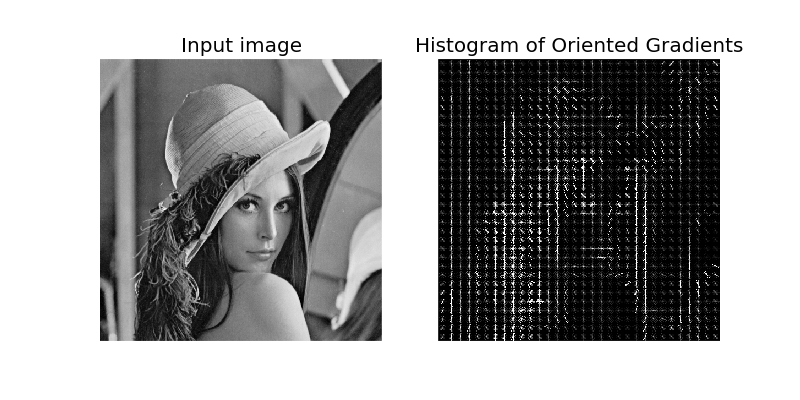
\includegraphics[width=11cm]{hog}
 \caption{Histogram of Oriented Gradients}
 \label{fig:hog:1}
\end{figure}

\section{Supervised Learning}
Supervised learning is a machine learning strategy where the target solution is presented after each training iteration. This differs from unsupervised learning in that unsupervised learning has no direct target to learn from, and is used to find underlying commonalities or patterns in data. \par
Supervised learning is the most commonly used method for image and video tasks, as typically the objective is to perform tasks where the target is well-defined. Common supervised learning tasks are \emph{image classification} - where the objective is to assign an input image a label from a fixed set of categories; \emph{localisation} - where the objective is to produce the coordinates of an object of interest from the input image; and \emph{detection} - which combines the previous two tasks. The task of localisation is actually a specific use-case for \emph{regression}, where the system is to predict a real-valued scalar given some input - used frequently for finance and weather prediction among other tasks. \par
There are a multitude of supervised and unsupervised learning problems, with  almost all meta-learning strategies targeting supervised learning. Due to this -- and that supervised learning has clearer, more measurable results -- I will focus primarily on the supervised task of image classification using neural networks. \par


\section{Optimisation}
\subsection{Loss} \label{loss:1}
The process of optimising a machine learning system is to present it with a target of some sort -- either in the supervised or unsupervised setting -- and compute a numerical quantity called \textit{loss} or \textit{cost}. This is a scalar value which is representative of how ``badly'' the system has performed inference given the input image. It is the system's objective to minimise this value through some optimisation algorithm. The loss function is specifically chosen for the task at hand, \textit{cross-entropy} being a common choice for image classification tasks and \textit{mean-squared (L2) error}  for regression. \\

\subsubsection{Symbols}
Before discussing loss functions, it's important to understand the inputs and outputs of a machine learning system when performing image classification. \par
For a system that makes predictions between $N$ classes, its input is a vector of image features $\bm{x}$ - usually the raw pixel values. The system's output is a vector $\bm{\hat{y}}$ of length $N$, where each of the output values $\bm{\hat{y}}_i$ is a score for class $i$ being the correct answer. The loss $\mathcal{L}$, as described above, is a function of the predictions $\bm{\hat{y}}$ and the target values $\bm{y}$. The target values are typically encoded as a \textit{one-hot} vector of length $N$, which is all zeros with a 1 in the position of the correct class. \\

\subsubsection{Softmax}
As the system's raw outputs aren't normalised and thus cannot be interpreted as a true confidence measure, the outputs normally go through a softmax function $\sigma$.
\begin{equation} \label{softmax:1}
 \sigma(\bm{\hat{y}})_i = \frac{e^{\hat{y}_i}}{\sum_{k=1}^{N}e^{\hat{y}_i}} \\
\end{equation}
The softmax function (eq \ref{softmax:1}) squashes the arbitrary scores into a vector such that its values sum to $1$ and are each in the range $[0, 1]$. The resultant values can be interpreted as the probability of the input image falling into each of the classes. Figure \ref{fig:softmax:1} shows the raw, unscaled predictions from a classification network (red), and the results of applying the softmax function (green). \par
\begin{figure}[h]
 \centering
 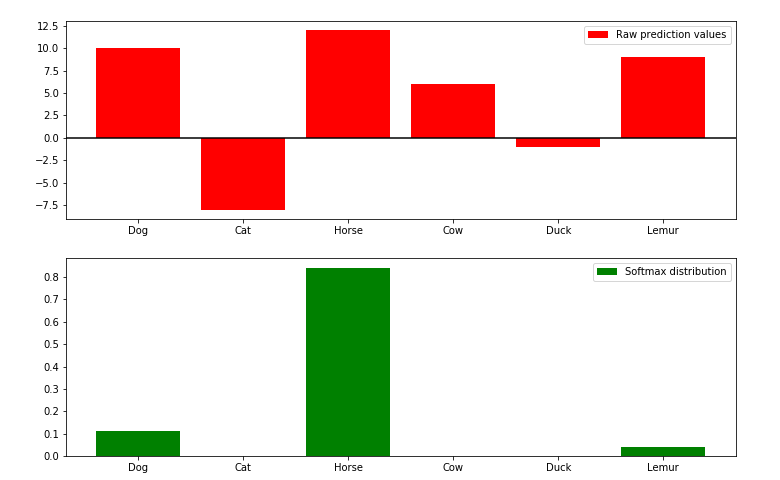
\includegraphics[width=12cm]{softmaxplot}
 \caption{The Softmax function applied to classification outputs}
 Note how the softmax function preserves the ordering of prediction values while emphasizing their differences, and gives the required properties of a probability distribution.
 \label{fig:softmax:1}
\end{figure}

\subsubsection{Cross-Entropy Loss} \label{crossentropy}
With the machine learning system producing a normalised probability distribution across classes, those values need be compared with the targets to produce a scalar loss value.
Cross-entropy loss, otherwise known as \textit{log loss}, penalises differences between predicted values and targets, with the penalty growing harsher for further-away predictions as demonstrated in fig \ref{fig:cross-entropy:1}.\\
For a vector of predictions $\bm{\hat{y}}$ and a one-hot target vector $\bm{y}$, the cross-entropy loss is:
\begin{equation} \label{cross-entropy:1}
 H(\bm{\hat{y}}, \bm{y}) = - \sum_{k=1}^{N}y_k log(\hat{y}_k) \\
\end{equation}
For the special case of \textit{binary} cross-entropy (as shown in fig \ref{fig:cross-entropy:1}) where number of classes $N$ is 2, the network's outputs are generally reduced to a single scalar value and cross entropy calculated as:
\begin{equation} \label{cross-entropy:2}
 H(\hat{y}, y) = -(y log(\hat{y}) + (1 - y)log(1-\hat{y})
\end{equation}
\begin{figure}[!h]
 \centering
 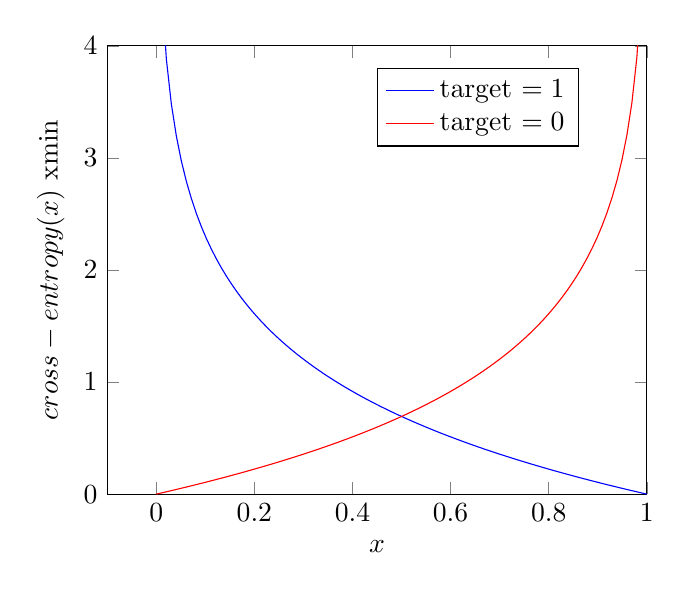
\begin{tikzpicture}
  \begin{axis}[
   xlabel=$x$,
   ylabel={$cross-entropy(x)$}
   xmin=0, xmax=1,
   ymin=0, ymax=4,
   legend style={at={(0.5,0.95)},anchor=north west}
   ]
   \addplot[domain=-0.01:1, color=blue, samples=100]
   {-ln(x)};
   \addplot[domain=0:1, color=red, samples=100]
   {-ln(1 - x)};
   \addlegendentry{target $=1$}
   \addlegendentry{target $=0$}
  \end{axis}
 \end{tikzpicture}
 \caption{Binary Cross-Entropy}
 \label{fig:cross-entropy:1}
\end{figure}

\subsubsection{Mean-Squared Error (L2)}
Mean-squared error is used for regression tasks, where the objective is to predict a quantitative value rather than a measure of probability. As L2 loss minimises the average error between the predictions $\bm{\hat{y}}$ and targets $\bm{y}$, the system learns to make predictions which lie in the mean position of these, which is generally ideal for regression tasks where there is one solution.\\
\begin{equation} \label{mean-squared-error:1}
 L2(\hat{\bm{y}}, \bm{y}) = \sum_{k=1}^{N}(y_k - \hat{y}_k)^2
\end{equation}

\section{Neural Networks}
Artifical Neural Networks (\textit{ANNs}) are machine learning systems loosely inspired by the functioning of the biological neural networks of the brain. They are composed of artificial neurons which transmit signals from one another in the form of a non-linear function of the sum of the incoming inputs. ANNs model unknown functions of arbitrary complexity, with their representational power a function of their size. \par
If we look at the structure of the simplest neuron possible $f_1$ (figure \ref{fig:neurons:1}a) we see that it is composed of two components - a weight $w_1$ and a bias $b_1$. Passing a value $x$ through a neuron $f_1$ is equivalent to computing the linear function $f_1(x) = w_1x + b_1$. The output of a neuron is known as its ``activation'' -- how excited the neuron was, given that input.
If the outputs of this neuron are then passed into a similar neuron $f_2$, we end up with the composite function
\begin{align}
 (f_2\circ f_1)(x) & = (w_2(w_1x + b_1) + b_2) \\
                   & = w_2w_1x + b_1w_2 + b_2
\end{align}
which is still a linear function of $x$. This is true for any number of sequential neurons, meaning that any composition of linear neurons is only as good as a single neuron. Having the capacity to produce linear relationships is only useful if the function being modelled is, itself, a linear function. For more complex modelling tasks -- which are encountered more often than not -- non-linearities need to be introduced into the network. In making a neuron a non-linear function, the problem with composite functions noted above no-longer exists; adding additional neurons does increase the representational power of the model. \par

\subsection{Activation Functions / Non-Linearities}
Activation functions (also known as non-linearities) are a critical component of neural networks as they add the capacity to model non-linear relationships. The inspiration for activation functions is drawn -- once again -- from the operation of biological neural networks, where neurons are only ``activated'' given sufficient input signal. In modern neural networks, only a few activation functions are regularly used: \par


\begin{itemize}
 \item\textbf{Sigmoid} $= \frac{1}{1 + e^{-x}}$ : The Sigmoid activation function (also known as the \textit{logistic function}) has the nice property that $(\forall x \in \mathbb{R}) Sigmoid(x)\in(0, 1)$ which is useful as a way of normalising values, especially when the output is to be interpreted as a probability.

 \item\textbf{TanH} $= \frac{e^{2x} - 1}{e^{2x} + 1}$ : The hyperbolic tangent function has similar properties to sigmoid, but maps numbers to the range $(-1, 1)$.

 \item\textbf{ReLU} $= \begin{cases}
 0, & \text{if } x < 0 \\
 x, & \text{if } x \ge 0 \\
 \end{cases}$
 The Rectified Linear Unit maps numbers to the range $[0, \infty)$ and has the advantage that it is much more computationally efficient than the above two activation functions; in most cases it yields better results.
 \item\textbf{Leaky ReLU} $= \begin{cases}
 0.01x, & \text{if } x < 0 \\
 x, & \text{if } x \ge 0 \\
 \end{cases}$
 The Leaky Rectified Linear Unit operates like ReLU, but allows numbers less than zero to ``leak'' through - this is in aid of \textit{backpropogation}, which is discussed at length in section \ref{backprop:1}.
\end{itemize}

\subsection{Fully-Connected Layers} \label{fully-connected:1}
The arrangement and structure of neurons discussed thus far hasn't been very practical, in that we were only considering a chain of continuous neurons one after another with just one input and output. Neurons will typically receive multiple inputs and produce a weighted sum of those inputs (fig \ref{fig:neurons:1}b). A neuron given $N$ inputs $\bm{x} = (x_1, x_2, ..., x_N)$ with weights $\bm{w} = (w_1, w_2, ..., w_N)$ and bias $b$ would then form the linear equation $w_1x_1 + w_2x_2 + ... + w_Nx_N + b$. \textit{For our purposes we will consider the activation function to be inside each neuron, although in practice they are applied in a layered manner.} \par
For a system consisting of multiple inputs, we want to allow diverse interactions between them. This is achieved by what's known as a \textit{Fully-Connected Layer} of neurons, where each output from the previous layer is passed as input to each of the following layer's neurons. Networks are generally grouped into layers to provide a nice abstraction from the hundreds or thousands of neurons inside. The layer architecture of neural networks means that each layer can be considered a stand-alone block, a black box with a mapping from an an arbitrary input size to an arbitrary output size. They can therefore be stacked one after another to form a \textit{fully-connected neural network} - see figure \ref{fig:neurons:1}c for an example. \par
A valid interpretation of the weights in a neural network is to consider them a measure of the importance of the inputs for the corresponding output. For example, a network which predicts the price of a house given the number of bedrooms; square metres; and the window-thickness, will likely have a very small weight for the window-thickness as it's not very \textit{important} to the price prediction. This is a very literal example, and with more complex tasks such as image classification the weights are not as easily interpretable. \par
\begin{figure}[h]
 \centering
 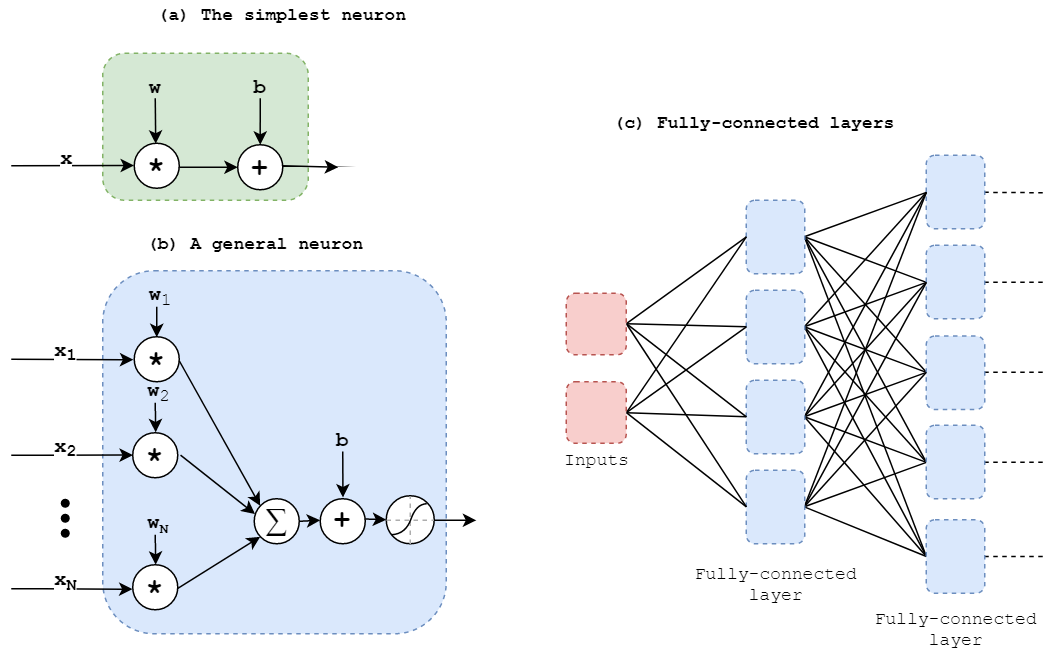
\includegraphics[width=14cm]{neurons}
 \caption{Neurons and fully-connected layers}
 \label{fig:neurons:1}
\end{figure}

\subsection{Stochastic Gradient Descent (SGD)} \label{sgd:1}
An ANN begins with randomly generated weights and biases $\bm{W}$ and $\bm{B}$, which are collectively referred to as the ``parameters'' or ``weights'' and indicated by $\bm{\theta}$. The objective of an ANN is to select weights $\bm{\theta}$ that minimise the error computed by the loss function $\mathcal{L}$ (section \ref{loss:1}). Linear functions $f(\bm{x}, \bm{\theta})$ can be minimised by analytical techniques, but complex neural networks must be iteratively optimised by numerical methods. \par
With the loss between a prediction $\hat{y}$ and target $y$, we can compute the gradients with respect to the parameters -- which essentially represents the direction of change which will result in a decrease in the loss value -- and make a small step in that direction (see figure \ref{fig:grad-descent:1}). When performing this operation over the entire dataset at once, this is known as gradient descent. This is usually not an option as the computational resources required for full gradient descent are prohibitive. If we instead repeat this operation for different examples until we have stabilised the loss to a low value, we have Stochastic Gradient Descent. The most common variant to this technique is known as Batch Gradient Descent, where instead of computing the loss and performing an update to the parameters on a per-example basis, the process is applied once per \textit{batch} of examples. It facilitates more stable learning, as the loss doesn't fluctuate as much as between single examples. Batch Gradient Descent is the basis for most ANN optimisation, although we'll discuss modern variants in section \ref{optimizers:1}. \par
\begin{figure}[h]
 \centering
 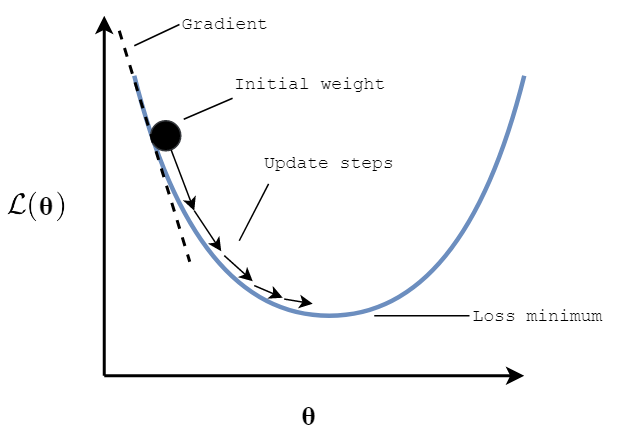
\includegraphics[width=9cm]{graddescent}
 \caption{Gradient descent updates}
 \label{fig:grad-descent:1}
\end{figure}

\subsection{Gradients and Backpropagation} \label{backprop:1}
We shall consider a general ANN $\sigma$ with $2$ fully-connected layers $f_1, f_2$ parameterised by $\bm{\theta} = \{\bm{\theta}_1, \bm{\theta}_2\}$ which can be represented as:
\begin{align} \label{gradients:1}
 \bm{\hat{y}} = \sigma(\bm{x}, \bm{\theta}) = f_2(f_1(\bm{x},  \bm{\theta}_1), \bm{\theta}_2)
\end{align}
That is, the input $\bm{x}$ is fed through layer $f_1$ then $f_2$. We will also consider an arbitrary loss function $\mathcal{L}$ which compares the predictions $\bm{\hat{y}}$ with targets $\bm{y}$ and produces a scalar loss value:
\begin{align}
 \mathcal{L}(\bm{\hat{y}}, \bm{y})
\end{align}
As the input $\bm{x}$ and target $\bm{y}$ is fixed, we may only change the parameters $\bm{\theta}$ to improve the loss. As explained in section \ref{sgd:1}, we wish to make incremental changes to our parameters where each change decreases our loss value. We do so by computing the gradient of the loss value with respect to the parameters:
\begin{align}
 \frac{\partial\mathcal{L}(\bm{\hat{y}},\bm{y})}
 {\partial\bm{\theta}}
\end{align}
If we are to find the gradients of the loss function with respect to the final layer's weights, we will have the equation
\begin{align}
 \frac{\partial\mathcal{L}(\bm{\hat{y}},\bm{y})}
 {\partial\bm{\theta}_2}
\end{align}
which is considered to be easily calculable. However, if we wish to find the gradient of weights further towards the start of the network, we cannot work those out directly and instead need to make use of the differentiation chain rule: \par
\begin{align}
 \frac{\partial f}{\partial x} = \frac{\partial f}{\partial u} \frac{\partial u}{\partial x}
\end{align}
To find the gradient of the loss function with respect to the first layer's weights, and considering that $\frac{\partial\mathcal{L}(\bm{\hat{y}},\bm{y})}
{\partial\bm{\theta}_2}$ is calculable, we simply need apply the chain rule as such:
\begin{align}
 \frac{\partial\mathcal{L}(\bm{\hat{y}},\bm{y})}{\partial\bm{\theta}_1} =
 \frac{\partial\mathcal{L}(\bm{\hat{y}},\bm{y})}
 {\partial\bm{\theta}_2}
 \frac{\partial\bm{\theta}_2}
 {\partial\bm{\theta}_1}
\end{align}
That is, once we know the gradient of the loss with respect to the second layer's weights, we can compute the gradient of the second layer's weights with respect to the first layer's weights and multiply the two to find the gradient of the loss with respect to the first layer's weights. This generalises to neural networks with any number of layers of differing types. This is an intuitive relationship, as we are essentially calculating the compound contribution that a change in any one parameter's value will have on the final output -- the loss.  \par
This technique used since the 1970s is aptly named \textit{backpropagation of error gradient}\parencite{backprop}, as it involves the propagation of the gradient of the error -- or loss -- from the end of the network back. \par
Returning to the concept of SGD (section \ref{sgd:1}) which was introduced on a conceptual level, we can now delve deeper into the application of the algorithm. Assuming that we have computed the gradient of each parameter in the network for the given examples in our batch, we can visualise this as a ``loss landscape'', whereby moving the parameters down-hill results in a reduction in the loss. Adjusting a parameter by the negative of the gradient will result in a ``step'' that moves the parameter closer to a local minimum with the objective to reach the lowest point possible, which represents the set of parameters resulting in the lowest loss. A configurable hyper-parameter is the \textit{learning-rate}, commonly represented by $\alpha$, which is the ``size'' of the step to take - that is, the coefficient of the negative of the gradient to apply (eqn. \ref{fig:sgd:1}). \par
\begin{align} \label{fig:sgd:1}
 \bm{\theta} = \bm{\theta} - \alpha \Delta_{\bm{\theta}} \mathcal{L}(\bm{\theta}, \bm{\hat{y}}, \bm{y})
\end{align}
\textit{For brevity we will from now write the gradient of the loss function $\mathcal{L}$ with respect to the parameters $\bm{\theta}$ as $\Delta_{\bm{\theta}} \mathcal{L}(\bm{\theta})$.} \\
The problem that is quickly encountered is how large a value to set the learning rate $\alpha$. Too small a step and it will take a long time to reach a minimum; too large and you may over-shoot it (see figure \ref{fig:learning-rate:1}). The example in figure \ref{fig:learning-rate:1} is a very low-dimensional loss landscape where the correct direction to move seems very logical, but higher dimensional spaces with a greater number of parameters result in complex landscapes with many local minima. We also want to slow down when nearing the bottom of a minimum so we can properly reach the lowest point. If we take this into consideration, and the fact that for any mini-batch the loss landscape will be different due to noise in small sample sizes, choosing a fixed learning rate becomes problematic. In practice, many people simply set up a learning rate schedule, where they decrease the learning rate at intervals, but it is hard to get right. It is with this in mind that adaptive optimizers came about. \par
\begin{figure}[h]
 \centering
 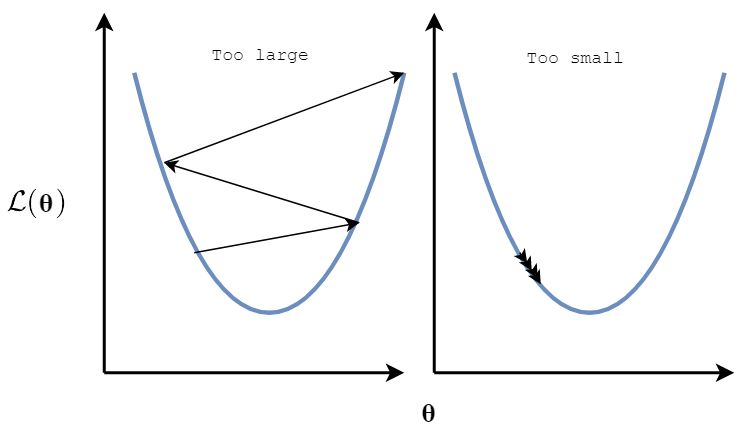
\includegraphics[width=10cm]{learningrate}
 \caption{Learning rate values}
 \label{fig:learning-rate:1}
\end{figure}

\subsection{Adaptive Optimizers} \label{optimizers:1}
If we consider a dataset where each mini-batch has some noise but that there is an optimal parameterisation for the entire set, we could visualise the loss landscape as shifting slightly for each mini-batch, but where there is a common direction towards which most samples will lead. Standard SGD will just apply a fixed step-size for all updates which leads the parameters to oscillate along the greatest descent angle, regardless of past updates. \par

\subsubsection{SGD with Momentum}
It is with the idea of a consistent optimization direction that momentum \parencite{backprop} comes into play. This is a technique of updating parameters while taking past updates into consideration to find the ``common direction'' in which to move. This is done by using an update vector which intuitively acts like the momentum of a ball rolling down a hill. For any update step, the direction vector is updated with a scaled contribution from the current gradient direction, and that vector is used to update the parameters. It essentially dampens oscillating movement, as the direction vector compounds contributions in the same direction as given in the following equation
\begin{align}
 \bm{v}_t      & = \gamma \bm{v}_{t-1} + \alpha \Delta_{\bm{\theta}} \mathcal{L}(\bm{\theta}) \\
 \bm{\theta}_t & = \bm{\theta}_{t-1} - \bm{v}_t
\end{align}
where $\gamma$ is the momentum term which indicates how much movement we wish to carry forward from previous time-steps.

\subsubsection{Nesterov Accelerated Gradient Descent} \label{nesterov}
If we consider momentum to compound the previous slopes such as a ball rolling down a hill, we end up with a problem where the momentum may cause the parameters to overshoot the minimum. Nesterov Accelerated Gradient Descent \parencite{nesterov} pre-emptively considers post-step parameters and makes adjustments to the step \textit{actually} taken. It does so by approximating the position after a momentum parameter update ($\bm{\theta} - \gamma\bm{v}_{t-1}$), and computing the loss gradient not with respect to the current parameters, but approximate future position. This optimisation strategy essentially glances into the future and makes a pre-emptive correction.
\begin{align}
 \bm{v}_t      & = \gamma \bm{v}_{t-1} + \alpha \Delta_{\bm{\theta}} \mathcal{L}(\bm{\theta} - \gamma\bm{v}_{t-1}) \\
 \bm{\theta}_t & = \bm{\theta}_{t-1} - \bm{v}_t
\end{align}

\subsubsection{Adagrad}
Adagrad \parencite{adagrad} is the first of the true ``adaptive'' optimizers, in that it adjusts the learning rate on a per-parameter basis, taking past gradients into consideration. The Adagrad update rule is
\begin{align} \label{adagrad:1}
 \theta_{t, i} & = \theta_{t-1, i} - \frac{\gamma}{\sqrt{g_{t, i} + \epsilon}} \mathcal{L}(\theta_{t, i})
\end{align}
where $\theta_{t,i}i$ is the $i$th parameter at time-step $t$, $\gamma$ is the learning rate, $g_i$ is the square of the sum of the squares of the gradients with respect to $\theta_{t,i}i$ up to step, $\epsilon$ is a small number to avoid dividing by zero, and $\mathcal{L}(\theta_{t,i}i)$ is the gradient of the loss with respect to $\theta_{t,i}i$. This optimizer has the benefit that while rarely performing as well as SGD with well-chosen hyperparameters, the default learning rate of $0.01$ consistently yields very good results.

\subsubsection{Adadelta and RMSprop}
The accumulation of squared gradients in the denominator of Adagrad means that that the learning rate continues shrinking and eventually becomes small enough to entirely stop training. Adadelta \parencite{adadelta} seeks to resolve this by instead of storing the accumulated sum of squared gradients, keeping a running average
\begin{align}
 E[g^2]_{t, i} = \gamma E[g^2]_{t-1, i} + (1 - \gamma)g^2_{t, i}
\end{align}
and updating equation \ref{adagrad:1} to be
\begin{align}
 \theta_{t, i} & = \theta_{t-1, i} - \frac{\gamma}{\sqrt{E[g^2]_{t, i} + \epsilon}} \mathcal{L}(\theta_{t, i})
\end{align}
RMSprop \parencite{rmsprop} is in effect identical to Adadelta, and were both developed to address the diminishing learning rate problem of Adagrad.

\subsubsection{Adam} \label{adam:1}
Adaptive Moment Estimation (Adam) \parencite{adam} builds from the previous adaptive optimizers by not only storing exponentially decaying averages of past squared gradients $v_{t,i}$, but by also keeping an exponentially decaying average of past gradients $m_{t,i}$ -- note the lack of the word ``squared''.
\begin{align}
 m_{t, i} & = \beta_1 m_{t-1, i} + (1 - \beta_1)g_{t, i}   \\
 v_{t, i} & = \beta_2 v_{t-1, i} + (1 - \beta_2)g^2_{t, i}
\end{align}
where $\beta_1$, $\beta_2$ are hyper-parameters for the proportion of past information carried forward, with the default values typically working well in practice. Replacing $E[\bm{g}^2]$ with $\bm{v}$, $\mathcal{L}(\bm{\theta})$ with $\bm{m}$, and a small change to the square-root we end up with
\begin{align}
 \theta_{t, i} = \theta_{t-1, i} - \frac{\gamma}{\sqrt{v_{t, i}} + \epsilon} m_{t, i}
\end{align}
While not the most recent (I have omitted a few other adaptive optimizers), Adam is rapidly becoming the most frequently used optimizer for its consistent convergence and ease-of-use.

\section{Dealing with Small Training Data Sets}
Gathering a large dataset can be very costly or impractical, with neural-networks regularly requiring hundreds or thousands of examples to learn anything. Due to the difficulty in obtaining data, many approaches have been devised to allow the training of neural networks with small datasets. \par

\subsection{Overfitting}
Likely the biggest problem with training on a small dataset is overfitting, which occurs when a model is trained on a small number of sample images. As mentioned earlier, it is desirable for a system to be shown enough images to determine which aspects of an image are characteristic of the class, and which are noise in the provided sample. Overfitting is when the model learns -- and becomes dependant on -- features specific to the training data provided that don't generalise well outside of that. \par
The effect of overfitting is that the model achieves a significantly lower accuracy when making predictions for previously-unseen images. When training on  a small training-set, overfitting can occur very easily, as models can learn features of the training images that are specific to those alone. When working with a larger training-set, the model typically sees enough variation in provided examples to gain a good approximation for the distribution of images within each class. \par
A model's capacity plays a large role in appropriately fitting to a dataset. If the model has too many parameters, it can learn to ``remember'' the images for each class to make predictions, and overfitting results. If the model has too few parameters, the model cannot draw a complex-enough boundary between classes, and underfitting results. Figure \ref{fig:fitting:1} shows an example of this with a simple classification task, with three levels of fitting. The best solution is in the middle, where the decision-boundary is mostly right for the seen data-points, but isn't too tight around them. The overfitting and underfitting examples draw decision boundaries such that any new data-points are less likely to fall on their respectively correct sides. \par
\begin{figure}[!h]
 \centering
 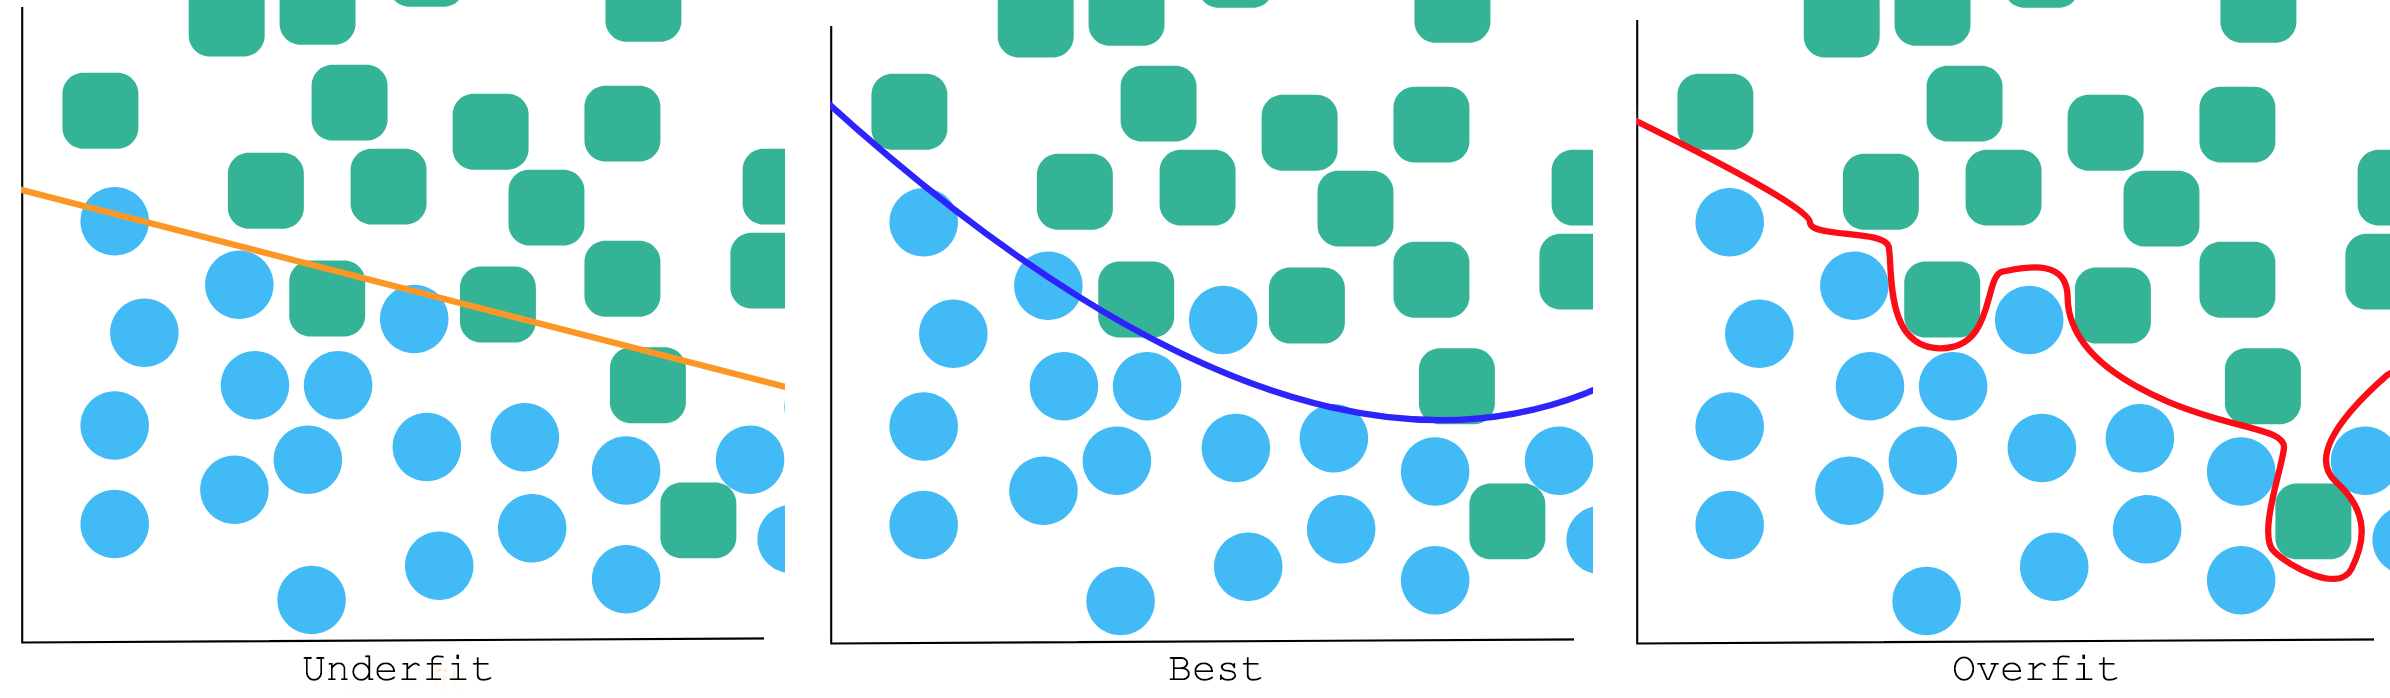
\includegraphics[width=14cm]{fitting}
 \caption{Levels of fitting for a simple classification task}
 \label{fig:fitting:1}
\end{figure}

\subsection{Transfer Learning} \label{transfer-learning}
Transfer learning is a commonly employed technique of taking a neural network that has already been trained on a similar task, and adapting its weights to the new domain. For image classification, this is done by downloading a pre-trained model, replacing the final fully-connected softmax output layer with a new output layer and training on the new dataset. There isn't always a necessity to re-train the entire model, as a large portion may be general-enough to apply to the new dataset. Due to this, the fine-tuning of models varies between adapting all parameters in the network, to the last few layers, to only the final softmax layer.  \par
The assumption that transfer learning hinges on is that the features learnt on a large dataset are general enough to transfer to a new, similar dataset. There are a number of well-known model architectures available for download, typically being trained on the \textit{ImageNet} image database\parencite{ilsvr}. \par
If the model is trained on a sufficiently large dataset it is true that the learnt features are usually general enough to receive good results after introducing relatively few samples from the new domain; but is not as effective as possible, especially when the new domain is significantly different from the old. As this approach requires the training of a model on a large source dataset, the user is either stuck with an existing model and no option to change, or must first train their own custom model on the large dataset first. This is a long, costly process which can be prohibitive. \par
Despite these limitations, transfer learning is the most effective and frequently-used technique for training on a new dataset when the amount of labelled data is small, achieving better performance than training on the new labelled data alone. \par

\subsection{Few-Shot Learning}
Few-shot learning is the ability to learn a new concept or idea from only a ``few'' examples. In the context of image-classification it is the ability to learn a new class from only a few example images. It's desirable to have a system that can learn from a small dataset, because -- as mentioned earlier -- it can be a long, costly process to label datasets. \par
The generalised description of few-shot learning for image classification is $N$-Way $K$-Shot learning, where $N$ is the number of classes between which the model is to make predictions and $K$ is the number of example images shown prior to having the model produce a prediction. Researchers tend to work on combinations of $N \in \{5, 10, 20\}$, $K \in \{1, 5\}$, regularly presented as one-shot and five-shot learning.

\subsection{Meta Learning}
Meta-learning can be described as ``learning to learn'', and in the field of computer vision is usually used to build systems able to adapt rapidly to new classes or domains. The goal in standard machine learning is normally to have a system that can generalise between examples within a domain, leveraging information seen in the training data to gain a generalised understanding of the data distribution. Meta-learning contrasts this in that the goal is to learn from the relationship between a data distribution and learning itself -- instead of being tightly bound to one specific domain. This is a sensible objective, as it's a trick humans use to speed-up the learning of new information. After being shown a photo of the proverbial zebra, it is quicker and easier to approximately learn it as a ``stripy horse'' rather than consider it an entirely new concept. \par
A \emph{meta-learner} is a system that's responsible for this external-observation -- with the learner playing the usual role -- however there are many designs without a distinction between the two. Meta-learning for few-shot problems is generally categorised into three different approaches:
\begin{itemize}
 \item \textbf{Optimization-based}: A model learns parameter update rules -- essentially replacing the role of an optimizer (section \ref{optimizers:1}) -- such that some good initial weights are modified rapidly and efficiently to perform well with the current set of images. These meta-learners typically employ an RNN (section \ref{rnn:1}).
 \item \textbf{Model-based}: A specific model architecture designed to handle few-shot problems by utilising some kind of memory unit -- typically an RNN (section \ref{rnn:1}), memory-network (section \ref{memory-nets:1}) or CNN with temporal-convolutions.
 \item \textbf{Metric-based}: A model learns a representation of the given sample images and a method by which to compare query images with the recently-provided sample(s).
\end{itemize}

\subsubsection{Training}
We will now consider the environment in which the aforementioned meta-learning approaches are trained and executed. \textit{Note that this section deals only with few-shot meta-learning for image-classification}. Having the system gain a meta-understanding of a task is almost exclusively approached in an episodic manner -- each episode consisting of conditioning a model on some examples of the task, having the model make a prediction, then updating the parameters to optimise this process. \par
As always in image-classification tasks, the dataset $\mathcal{D}$ is split into two class-disjoint sets $\mathcal{D}_{train}$ and $\mathcal{D}_{test}$, the latter a held-out set from which the model isn't allowed to learn. Additionally, as few-shot learning requires the exposure of examples before making a prediction, each of the sets is split on an episode basis into a \textit{support} set $\mathcal{D}_{S}$ and a \textit{query} set $\mathcal{D}_{Q}$. For the case of training five-way one-shot classification, the support set will consist of one image from each of five randomly selected classes from $\mathcal{D}_{train}$, with the query set consisting of one or more images drawn from the same dataset and belonging to one of the classes found in the support set (figure \ref{fig:episode:1}). The model is shown $\mathcal{D}_S$, optimizes itself for these classes, then is shown $\mathcal{D}_Q$ for which to make a prediction. The meta-learner observes this, and optimizes the process by which the learner adapts during each episode. \par
Due to the episode-based training, where the system sees a ``new'' set of classes in each, the meta-learner learns class-agnostic relationships between the support-set and the query-set. This then means that the meta-learner must persist knowledge between episodes, effectively learning an episode-invariant learning technique. This is validated by presenting an episode from $\mathcal{D}_{test}$ without the meta-learner's observation. \par
\begin{figure}[!h]
 \centering
 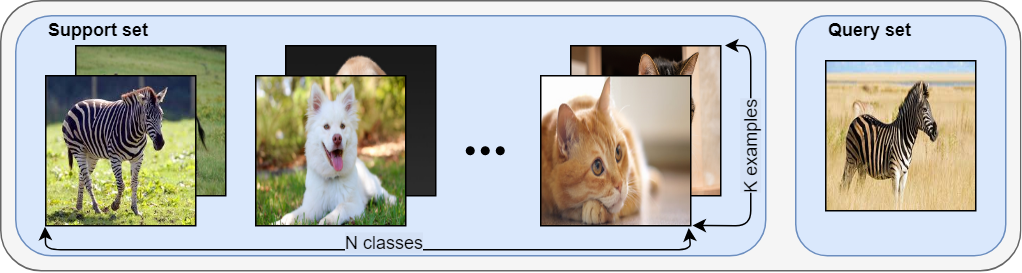
\includegraphics[width=14cm]{episode}
 \caption{An N-way K-shot training episode}
 \label{fig:episode:1}
\end{figure}

\section{Continuous Learning}
Learning from a continuous stream of new information is a crucial milestone in the development of artificial intelligence -- especially artificial \emph{general} intelligence -- as the normal offline-training procedure is impractical, and vastly different from biological neural networks. The neural networks found in the brain have the capacity for continuous learning -- the ability to learn new tasks/information without sacrificing previous skills/knowledge. ANNs don't have this capacity built-in, as the training typically occurs on a per-example (episode, image, batch, etc.) basis, with the purpose of optimising for that specific episode. It is inherent then, that a network will sacrifice its existing parameter state to perform better at the task presented. This forgetting of older knowledge when learning new information is known as \textit{catastrophic forgetting} or \textit{catastrophic interference}. \par
Catastrophic forgetting purportedly occurs when there is representational overlap inside a network between old and new information \parencite{hat}. The easiest way to gain an understanding of the new domain is to reuse that knowledge, sacrificing performance on the previous domain. This leads to an abrupt decrease in performance on the old domain, and eventually a total loss of learned knowledge. \par
There have been many attempts at mitigating catastrophic forgetting using as number of methods (section \ref{related-cont-learning:1}) with varying degrees of success; many drawing inspiration from the brain. Strategies include replaying older examples/tasks; freezing portions of the network's parameters; using loss functions designed to minimise forgetting; and adjusting the learning speeds for weights important for older tasks. \par
While this literature survey is not focused on neuroscience, we will briefly mention some of the known neurophysiological functions that allow the biological neural networks to adapt quickly to new information while retaining learnt information from previous tasks. \par
\begin{itemize}
 \item\textbf{Neurosynaptic plasticity} - The brain is particularly plastic during early development, allowing for sense-driven changes to occur on a large scale. Plasticity decreases with increasing age to provide stability, but a degree of plasticity is retained for small-scale adaptation.
 \item\textbf{Hebbian plasticity}\parencite{hebbian}\label{hebbian:1} - ``Neurons wire together if they fire together''\parencite{wirefire}. An observed pattern in the brain where synaptic efficacy (neuron firing strength) increases through persistent stimulation. Simply put, frequently used neural pathways gain strength and reduce plasticity.
 \item\textbf{Complementary learning systems} - As the brain's task is to both learn and memorise, it consists of two primary components relating to memory. The hippocampus rapidly encodes new memories into sparse representations for quick short-term recall with minimal interference, whereas the neocortex slowly encodes older memories into overlapping representations for long-term storage.
\end{itemize}
Researchers often return to the brain for inspiration due to its incredible capacity to deal with long-term memory without exhibiting catastrophic interference. However, the brain is far from fully understood, so proposed solutions in machine learning rapidly reach a limit of practicality. \par

\subsection{Class-Incremental Learning} \label{cil}
A specific set-up for the problem of continuous learning is \emph{class-incremental learning}, where a system is introduced new classes of information in a strictly incremental manner -- class $i$ is only shown to the system after it has seen class $i-1$ in its entirety. In some variations, classes may be introduced in sizes greater than one, adding five or more classes for each increment. Class-incremental learning is a good test of a system's capacity for continuous learning, as it only has the one opportunity to learn each class distribution but is to retain that information for ``life''. \par

\section{Modern Deep Learning Architectures} \label{modern-dl:1}
The only ANNs we've covered as of this point are \textit{fully-connected neural networks} (section \ref{fully-connected:1}) which have a very limited capacity in terms of practical use-cases, as we'll explore in this section. \par

\subsection{Convolutional Neural Networks} \label{cnn:1}
Let us consider a fully-connected network for classification on the popular dataset MNIST (figure \ref{fig:mnist:1}), with the raw pixel values fed in one side and a class probability distribution being output. Fully-connected layers need a single column (vector) of values as inputs, so we will first ``unwrap'' the image into a long string of pixel values before feeding it in. \par
\begin{figure}[h]
 \centering
 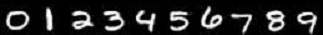
\includegraphics[width=6cm]{mnist}
 \caption{Ten examples from the MNIST dataset}
 \label{fig:mnist:1}
\end{figure}
Each input pixel would then be mapped by a distinct neuron weight in the first layer, which is problematic. Following the "importance weighting" interpretation introduced in section \ref{fully-connected:1}, the network must consider each input pixel individually with regards to its importance in the classification prediction. The same input image shifted by one pixel in any direction will likely produce very different results. This problem is inherent to fully-connected layers, and is best addressed by \textit{convolutional layers}. \par
We would instead prefer to see the image in a more global context, where we can learn about the presence or absence of features throughout the image. It's easier to describe the number eight as ``one circular thing on top of another circular thing'' than by raw pixel intensities. This was the work of hand-engineered \textit{kernels} for a long time prior to the resurgence of neural networks -- see figure \ref{fig:hand-eng-kernels:1} for examples of hand-engineered edge-detection kernels and their results. As kernels are a fundamental concept for convolutional neural networks, we'll now go into some detail. \par
\begin{figure}[!h]
 \centering
 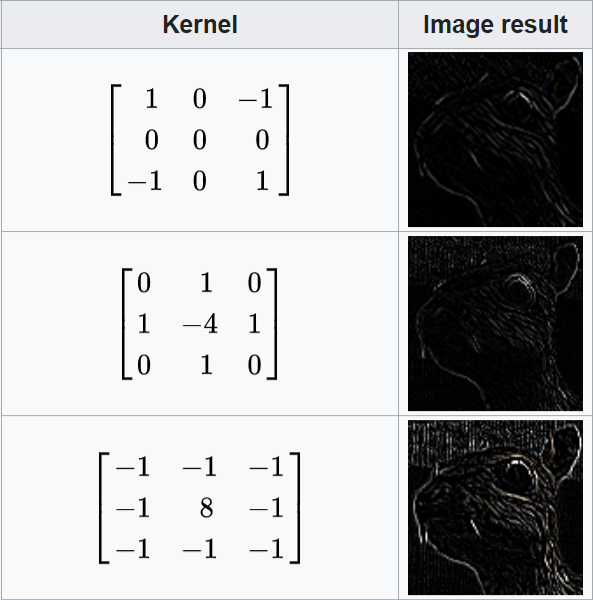
\includegraphics[width=8cm]{handengkernels}
 \caption{Hand-engineered edge-detection kernels}
 \label{fig:hand-eng-kernels:1}
 \textit{Image adapted from https://en.wikipedia.org/wiki/Kernel\_(image\_processing)}
\end{figure}
A kernel -- also known as a filter -- is a (typically square) matrix that is convolved over an input image to produce another image which contains some locally-aggregated information. It can be thought of as a window that slides over the image, seeing it in small sections. At each position the values in the input are multiplied by the corresponding point in the kernel, and the output value is their sum. Figure \ref{fig:kernel:1} shows a 3x3 kernel applied to a region of pixel values of a very small input image, and the resultant value. Their applicability to neural networks is very convenient, as all we need to do is replace the hand-engineered values with learnt weights and we have the makings of a convolutional layer. As discussed in section \ref{hand-eng:1}, hand-engineered features are usually of limited capacity, with data-driven features being more powerful. \par
\begin{figure}[!h]
 \centering
 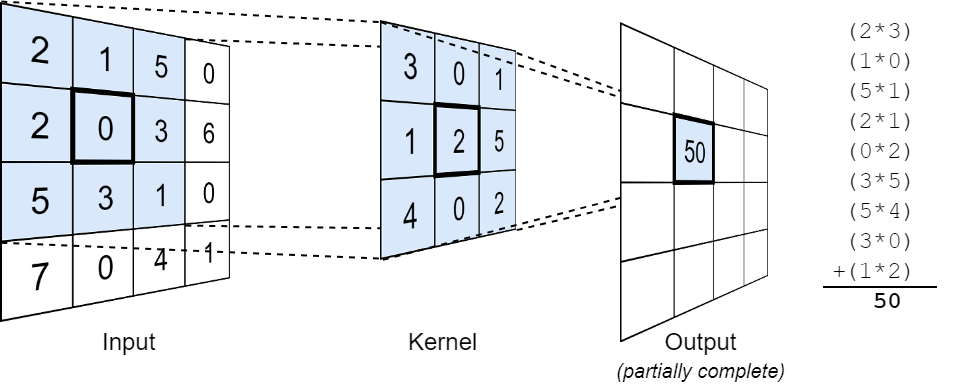
\includegraphics[width=12cm]{kernelimg}
 \caption{The calculation of a 3x3 kernel applied at one point}
 \label{fig:kernel:1}
\end{figure}
The outputs of a single kernel 3x3 convolutional layer are an image-like matrix which contains locally-aggregated information from the input image. As the kernel is 3x3 pixels, the \textit{effective receptive field} size at this point is 3x3 pixels. That is, each of the features in the outputs correspond to a 3x3 region of pixels in the inputs. If the outputs of this layer are fed into another layer of the same size, the effective receptive field size at this extra layer will be 5x5 pixels. The trend of an increasing receptive field continues for more layers, which has great consequences -- the further into a network of convolutional layers, the more global the information as the deeper filters can see more of the input image features. \par
It's important now to discuss what ``features'' are, as they're a key concept that have a fuzzy meaning. Image features extracted by data-driven convolutional kernels are unintuitive by nature, but we can build a sufficient understanding logically. Consider that through training our network, filters will be developed that respond to important features. These features will likely be things like horizontal lines; vertical lines; and soft gradients -- simple features. Subsequent layers will be dealing with not images but extracted features, so they will be responding to \textit{combinations} of features -- things like corners and more complex edges. As we proceed further into the network, the features learnt get more complex until we have filters responding to things like dog noses, text, wheels, etc. \par
With this knowledge that the depth of a neural network corresponds to its global understanding and its ability to learn complex features, it makes sense that modern convolutional neural networks are quite deep -- sometimes comprised of hundreds of layers. For the task of image classification, the missing link in the chain is how we produce the probability over the classes: take the outputs of the final convolutional layer, ``unwrap'' it as we did for the input image, and pass it through a fully-connected layer to produce the right number of output values. \par

\subsection{Recurrent Neural Networks}\label{rnn:1}
Nothing covered so far has had the capacity to work on variable length input and output data; Recurrent Neural Networks (RNNs) address this. We have only seen two sets of values relating to a neural network -- weights, which are the network's ``intelligence''; and activations, which are the neurons' responses to the given inputs. Only the weights persist between runs, but don't have the capacity to retain information about individual samples (if they do, they've overfit!). \par
For a neural network with a single hidden-layer, the activations at time $t$ are $h = \sigma(\bm{W}\bm{x}_t)$ for some input $\bm{x}_t$, weights $\bm{W}$, and activation function $\sigma$. RNNs work by recursively passing their hidden state through time-steps, weighted by learnt values. This can be expressed mathematically as
\begin{align}
 \bm{h}_{t} = \sigma(\bm{W}\bm{x}_t + \bm{U}\bm{h}_{t-1})
\end{align}
where $\bm{U}$ is a learnt matrix which filters and scales the hidden state values passed between time-steps. The recurrent design of this relationship means that not only will time-step $t$ contain information from time-step $t-1$, but $t-2, t-3, ...$ Figure \ref{fig:rnn:1} shows a very simple RNN. Note that we haven't discussed how to trigger an RNN to stop -- this is purposefully omitted as it's outside the scope of this writing. \par
By their design, RNNs are able to consider all prior information when making a prediction. This makes them a perfect candidate for time-series or arbitrary length sequence data such as text, weather predictions, speech-recognition etc.
\begin{figure}[h]
 \centering
 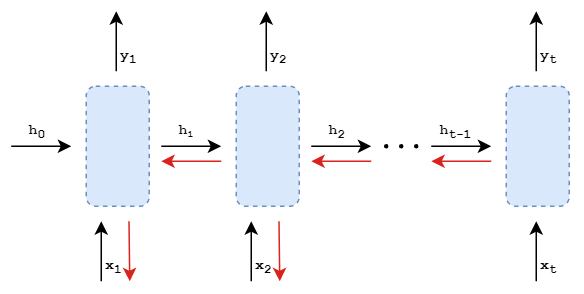
\includegraphics[width=12cm]{rnn}
 \caption{A simple Recurrent Neural Network}
 \label{fig:rnn:1}
 This network maps inputs $x_i$ to outputs $y_i$ for $i \in \mathbb{N}^{[1, t]}$. Red arrows indicate error-backpropagation.
\end{figure}

\subsubsection{Exploding/Vanishing Gradients}
When training an RNN, you typically need to see the entirety (or at least a large portion) of its outputs to compute the loss -- e.g. we can't assess how well it constructed a sentence until we can see the whole sentence. The training error is back-propagated through time from the last of the output sequence to the first of the input sequence (see the red arrows in figure \ref{fig:rnn:1}). \textit{The missing red arrow for input $x_t$ relates to the fact that we've omitted the ``stop'' trigger mentioned in section \ref{rnn:1}.} \par
As the gradients must be passed a long way, it is easy to imagine that we may end up with compounding errors, resulting in numerical instability. Gradients are particularly susceptible to this -- with the relationship between layers being multiplicative, any consecutive operations on values less than 1 approach zero, and any consecutive operations on values greater than 1 approach $\infty$. These problems are known respectively as the vanishing gradient problem, and the exploding gradient problem. Figure \ref{fig:multi-sigmoids:1} demonstrates this problem: with the sigmoid function being applied repeatedly we see that the output values ``flatline'' with the gradient rapidly approaching zero. As the gradients are used to propagate training error, no gradient means no learning.
\begin{figure}[h]
 \centering
 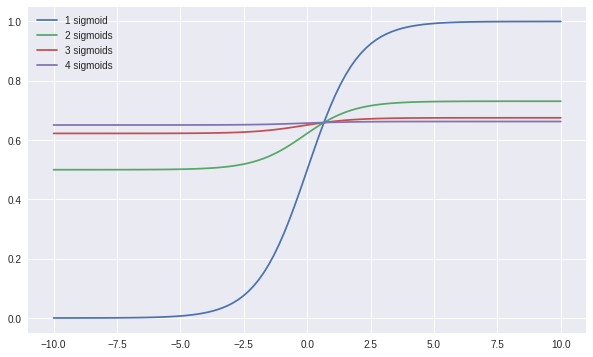
\includegraphics[width=10cm]{multi-sigmoids}
 \caption{The effects of applying the sigmoid function repeatedly}
 \label{fig:multi-sigmoids:1}
\end{figure}
\subsubsection{Long Short-Term Memory Units} \label{lstm}
Long Short-Term Memory Units (LSTMs) were proposed as a solution to the gradient problems inherent to RNNs. They have become so prolific and successful that usage of the acronym RNN generally refers to an LSTM instead. LSTMs mitigate the exploding/vanishing gradients problem by containing information outside of the normal hidden state of the network; the vanilla RNN approach doesn't really allow for dynamic usage of the hidden state. \par
LSTMS introduce a memory structure referred to as a \textit{gated memory cell}, which is similar to Random Access Memory on a typical computer -- information can freely be written, read, and erased out of order. However, while RAM supports digital reading/writing/erasing, LSTMs allow for \emph{analog} memory access -- data is changed and read to varying degrees in a differentiable process. There are a handful of variants on the LSTM which are growing in popularity, but as the internal workings of those and LSTMs are too complex to discuss in this writing, we won't explore them any further. \par

\subsection{Memory Networks}\label{memory-nets:1}
Although RNNs are designed for temporal data, they have been the architecture of choice for non-temporal, variable-length data for quite some time, as standard feed-forward networks don't have memory units. Memory networks address this by augmenting regular neural networks to have an addressable external memory unit. They operate in a different manner to LSTMs, but they share the same idea of gates managing the read/write/erasure of elements in their respective memory unit. We will briefly touch on how a memory network functions as it has great relevance to few-shot learning, where memory of past examples is helpful, but doesn't have a strict temporal relationship. A high-level view of memory networks (figure \ref{fig:memory-nets:1}) is as follows:
\begin{itemize}
 \item \textbf{Memory} - An indexed array of vectors representing the currently-stored information.
 \item \textbf{I}nput map - Transforms inputs to a unified internal feature representation.
 \item \textbf{G}eneralisation component - Updates old memories given new input. Referred to as ``generalsisation'' as this is responsible for compressing and generalising old memories into new representations.
 \item \textbf{O}utput map - Produces an output given the new input and the state of memory.
 \item \textbf{R}esponse component - Converts the output into the external representation such as text, prediction probability distribution, etc.
\end{itemize}
Memory networks have had significant success, and offer a practical alternative to RNNs when working with any variable-length data -- time-series based or not. The functionality of their memory unit has proven to perform better with long-term memory retention than even LSTMs. \par
\begin{figure}[h]
 \centering
 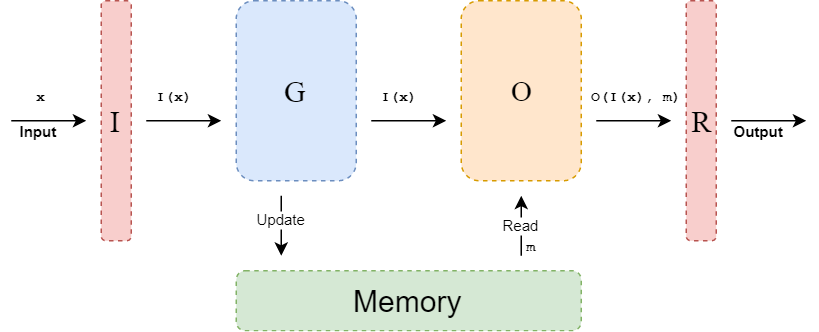
\includegraphics[width=14cm]{memory-nets}
 \caption{High-level overview of a memory network}
 \label{fig:memory-nets:1}
\end{figure}

\section{Summary}
In this chapter we introduced the concept of hand-engineered features, and how neural network architectures optimise this process so human-imposed knowledge doesn't limit the capacity of a system's performance. w then explained the functionality and applications of modern deep-learning architectures including CNNs; RNNs; and Memory Networks, and the problem domains within which we will be working. In the following chapter we will build on top of the background information described here, and analyse existing works in the fields of meta-learning and continuous learning. \par

\chapter{Related Works} \label{related:1}
As the problem domain spans across few-shot meta-learning and continuous learning, there is a myriad of related works of which we will introduce and summarise a selection. We will discuss the techniques used by each with a focus on their applicability to the task of few-shot continuous learning. We will then compare the results produced by each, with a closing discussion on the feasibility of their extension to the combined task. \par

\section{Few-Shot Meta-Learning}
The few-shot works discussed in this section represent a cross-section of most types of solutions, but especially those that closest relate to our problem. The techniques are broken into three sub-categories, \emph{model based}, \emph{metric based} and \emph{optimization based} -- each of which have their perks and downfalls, which are briefly mentioned at the end of each sub-section, and compared in section \ref{works:summary}. Few-shot meta-learning is usually considered separate to continuous-learning, so many of the approaches found in this section are less-applicable than others in the context of the problem defined in chapter \ref{problem-definition}.

\subsection{Model Based} \label{related-meta-modl:1}
Model based meta-learning techniques are those that base the solution around a specific model design. These are typically implemented with some sort of memory unit -- such as an LSTM or memory network -- though this isn't mandatory. Basing a solution on a custom model gives more freedom to design a task-specific system, but generally suffers as it can be difficult to change the architecture for different tasks. \par

\subsubsection{Learning to Learn with Backpropagation of Hebbian Plasticity}
The technique of Miconi et. al. \parencite{ltlwbohb} uses the theory of Hebbian plasticity (section \ref{hebbian:1}) to allow for connections between highly active pairs of neurons to increase in efficacy throughout their lifetime. This is achieved by defining a time-dependant quantity they call the ``Hebbian trace'', which acts as a moving-average of pair-wise synaptic activities. Using back-propagation, they train a plasticity parameter which determines how much the Hebbian trace influences the pair's connection; this plasticity parameter is fixed once trained. The Hebbian trace is computed during all forward-passes of the network throughout its lifetime, weighting the activations of neuron-pairs proportionate to their learned plasticity. \par
Although the technique described is primarily for continuous learning, they also apply it to a one-shot task. The task described is a toy-problem, but shows that through utilisation of the implemented Hebbian plasticity, the model is capable of quickly adapting its learning capacity to deal with the few-shot problem domain. The Hebbian trace could very easily be added into any artificial neural network architecture as an additional learned parameter. However, this technique's effectiveness at continuous learning tasks eventually becomes limited as the network's learned internal representation still remains fixed, meaning that there is no opportunity for it to consolidate knowledge as the breadth of the problem domain grows. \par

\subsubsection{One-shot Learning with Memory-Augmented Neural Networks}
One-shot learning is approached by Santoro et. al. \parencite{oslwmann} using a memory-augmented neural network (section \ref{memory-nets:1}). Memory networks are an ideal choice for few-shot learning, as they can rapidly encode, decode and selectively forget items from their external memory unit. The typical method for accessing memory locations is to use simple ``attention'', which allows the model to learn its own strategy. The authors of this paper recognise that this may result in an attention mechanism that is better purposed to sequential data, rather than the strictly un-ordered task of few-shot learning. They propose a novel memory access module called the Least Recently Used Access (LRUA) module, which is a content-based memory writer that writes memories to either the least-used or most-recently used memory locations, depending on the network's context. \par
This new access method garnered strong results, as it allowed the network to learn to replace unnecessary information as required. They show that the technique can be applied successfully to classification and regression problems, but identified that the memory unit must be cleared between tasks, lest proactive interference may occur. It must also be acknowledged that although the LRUA module achieves increased performance, it is still a complex hand-engineered solution which is not applicable to all problem domains, and is outperformed by simpler methods such as TCML (see below).  \par

\subsubsection{Meta-Learning with Temporal Convolutions}
At its core, the work of Mishra et. al. \parencite{mlwtc} devises a method which works in a purely causal manner -- the model is only influenced by previous time-steps. This is a clearly logical set-up for few-shot learning, as the task is to make decisions (specifically -- predict the class of an image) based on a small number of previously-unseen inputs. The term ``temporal convolutions'' refers to an adaptation of standard convolutions -- which convolve over coordinates -- such that the convolutions occur through time. The architecture is a deep stack of dilated temporal-convolutional layers -- where dilation basically refers to the ``overlooking'' of previous information, so as to have a larger temporal ``view'' without requiring a larger number of parameters (see the bold black diagonal lines in figure \ref{fig:temporal:1}). \par
\begin{figure}[h]
 \centering
 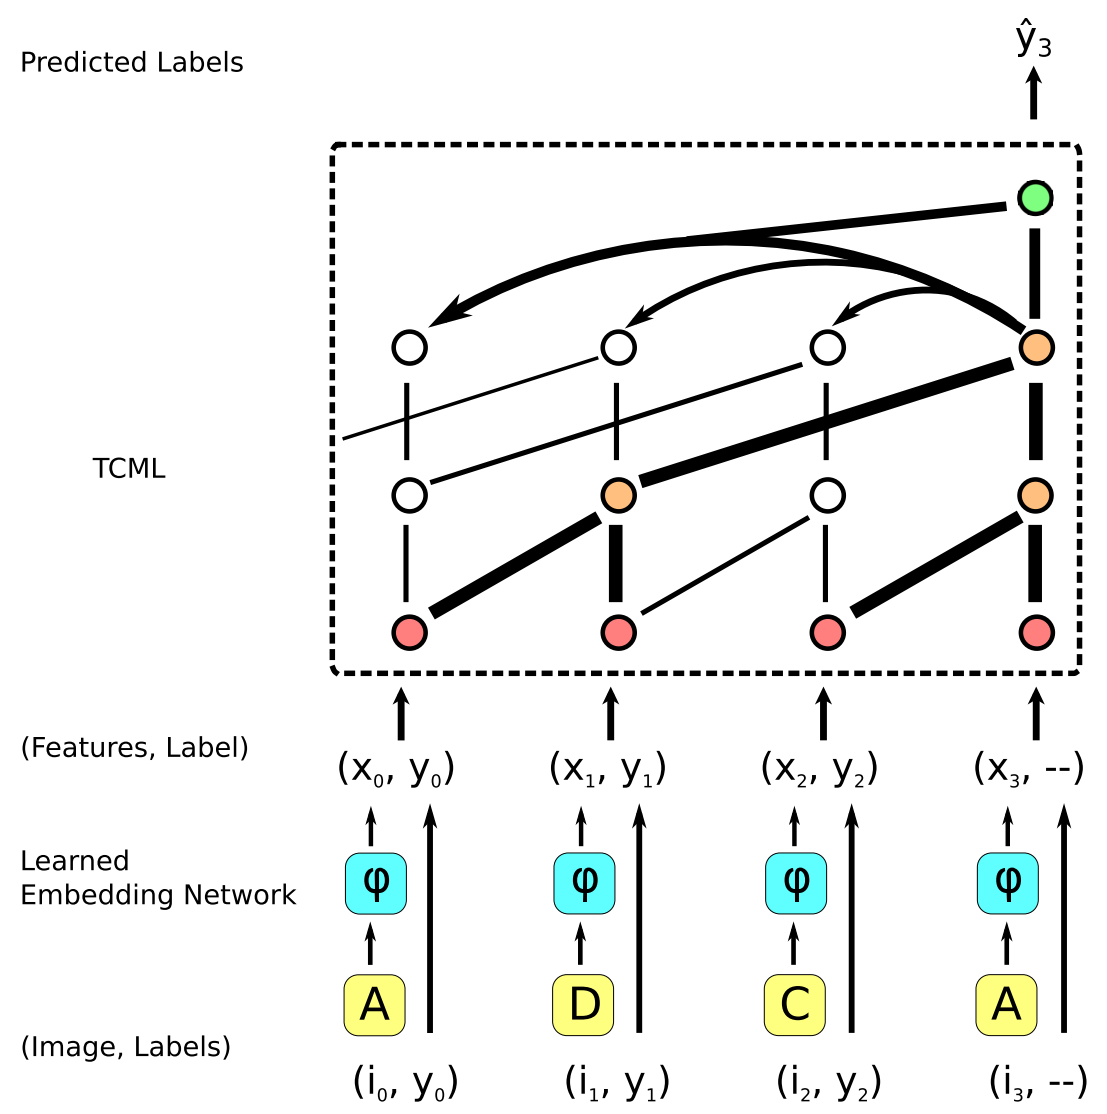
\includegraphics[width=9cm]{temporal}
 \caption{Temporal Convolutional Meta-Learner (TCML) system architecture}
 \label{fig:temporal:1}
 Support image/label pairs $(i_0,y_0), (i_1,y_1), ...$ are fed in one per time-step, then the query image without its label. Image features are extracted for each input, then the TCML outputs the label for the support image it associates with the query image.
\end{figure}
This approach works across many problem types including few-shot and reinforcement learning, but we will only consider few-shot learning. The inputs to the network are shuffled support images with their associated labels, and a final query image with an ``empty'' place-holder label. The model thereby learns an internal relationship between the support images and the query image, effectively computing finding the most similar. As the network uses dilated temporal-convolutions, the number $N_{support}$ of support images -- and therefore the number of classes between which the network can classify -- can be quite large, with the model needing only $log(N_{support})$ layers, as dilated convolutions give an exponentially-increasing temporal view.  \par
The results obtained by this technique are encouraging, achieving state-of-the-art results across the board. As with all approaches however, there are drawbacks. Other few-shot learning techniques (optimizer based - section \ref{related-meta-opt:1}, some metric based - section \ref{related-meta-metr:1}) perform a life-long update, meaning a usable classifier is produced after presenting support examples once only -- never needing to see those examples again. TCML (and most few-shot meta-learners) don't do this -- in order to perform classification, at least one example from each class must be presented alongside every query. Therefore the system's performance rapidly degrades with respect to the number of classification categories, making it an impractical choice for continuous learning. \par

\subsubsection{Meta Networks}
The so-called \emph{MetaNet} developed by Munkhdalai et. al. \parencite{mn} is somewhat an amalgamation of meta-learning techniques including memory networks and fast weight generation -- weights that are rapidly changed or generated dependent on network inputs. There is also a clear separation between the meta-learner and the base-learner, a line that is regularly indistinct with other techniques. \par
The base-learner is parametrised by slow weights updated via a typical learning algorithm during training, and example-level fast weights generated by the meta-learner for each input (see figure \ref{fig:metanet:1}a). The base learner computes the loss for its predictions for the support set, and gives the gradients to the meta-learner. The meta-learner takes this meta information and produces a set of fast weights for the base learner when training, as well as producing its own fast weights, as a function of the information stored in memory and the meta-information. The combination of slow weights with fast weights is shown in figure \ref{fig:metanet:1}b, where its shown that the weights work in parallel, with element-wise addition used to merge the activations. \par
\begin{figure}[h]
 \centering
 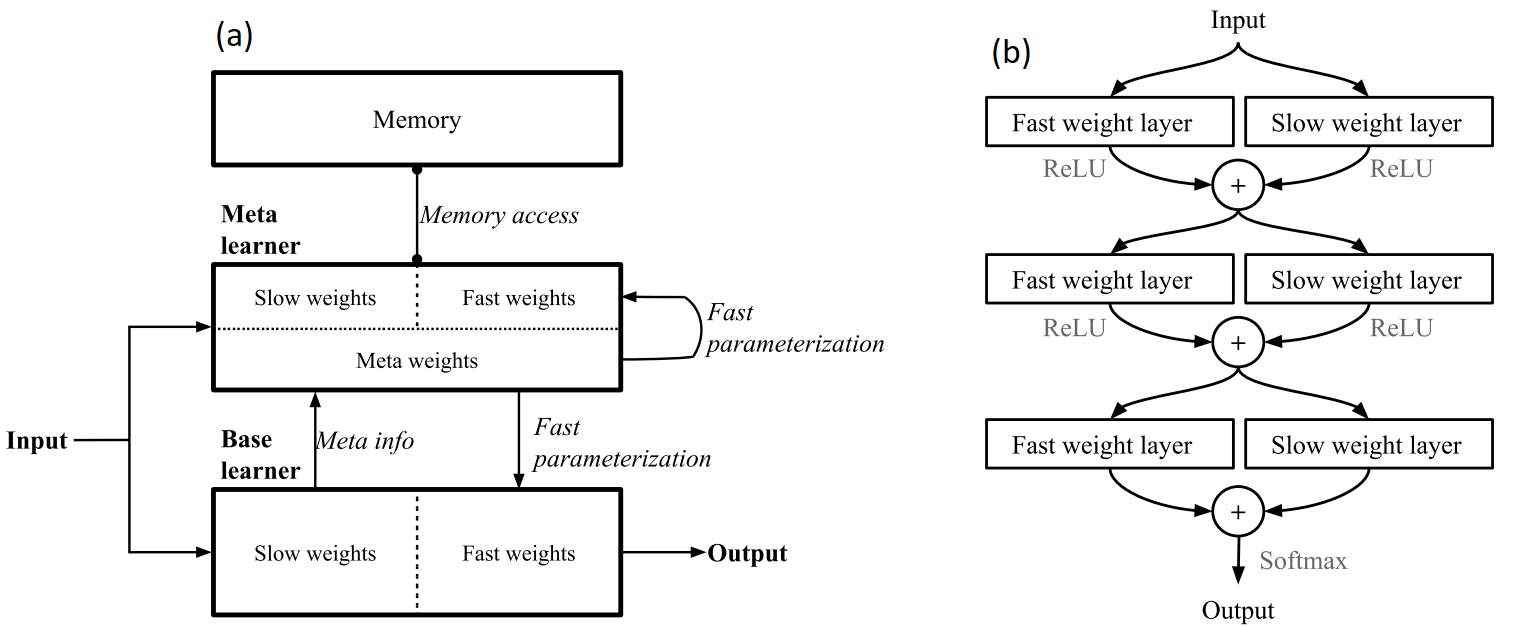
\includegraphics[width=15cm]{metanet1}
 \caption{Meta Networks system architecture}
 \label{fig:metanet:1}
\end{figure}
MetaNet achieves competitive results for common one-shot learning tasks, and even demonstrates positive reverse transfer as shown in figure \ref{fig:metanet:2}. This is ideal performance for a multi-task learner as it means that the meta-learner is good at persisting task-agnostic information, while incorporating newly found information. That being said, the model architecture is very complicated, with many co-dependencies between the base-learner and the meta-learner. This complexity -- and that MetaNet introduces a large number of parameters proportional to the base-learner's size -- makes it an undesirable choice for practical applications.  \newline \newline
\begin{figure}[h]
 \centering
 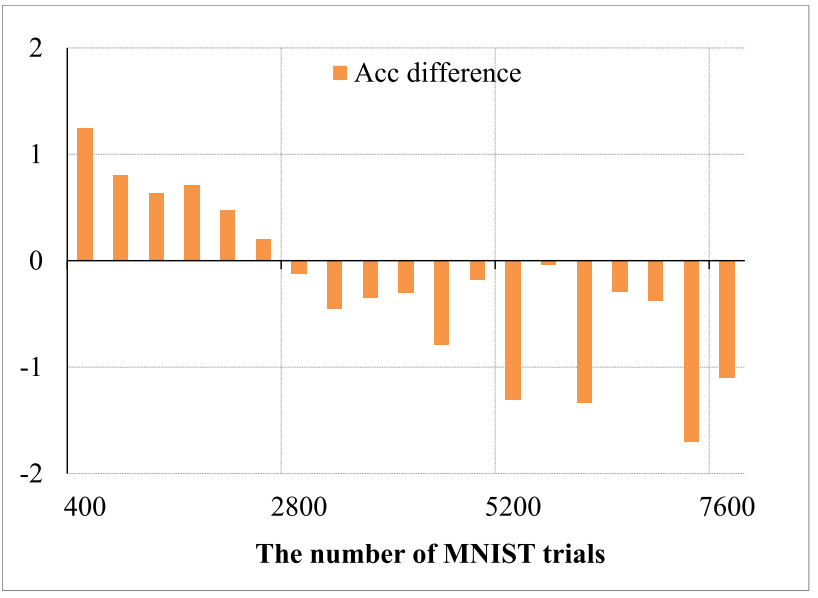
\includegraphics[width=8cm]{metanet2}
 \caption{Omniglot test accuracy change obtained while training Meta Networks on MNIST}
 \label{fig:metanet:2}
\end{figure}
Each of the works discussed in this section have had strong results for few-shot tasks, however none have much applicability to continuous learning, and many require complex implementations. An ideal system would allow for the adding of classes throughout time, without being restrictively difficult to implement. \par

\subsection{Metric Based} \label{related-meta-metr:1}
Metric based meta-learning solutions deal with embedding query and support images into a space and computing the similarity, or distance between them. These approaches are typically very simple and accurate, but suffer from the problem that the number of embeddings and comparisons generally grows proportionate to the number of classes. This can be partially avoided by pre-embedding support images, but means that models cannot be further trained without the embeddings degrading, making them poor candidates for continuous learning. \par

\subsubsection{Siamese Neural Networks for One-Shot Image Recognition}
The work by Koch et. al. \parencite{siamese} uses \textit{siamese neural networks} to learn an image similarity-measure. Siamese networks are a class of architectures that are primarily for the purpose of computing the similarity between pairs of images. Two images are fed separately into a network which embeds them into a vector of length 4096 (see figure \ref{fig:siamese:2}). The embeddings then have the absolute value of their difference computed, and are passed through a final fully-connected layer to produce a scalar similarity value. \par
\begin{figure}[h]
 \centering
 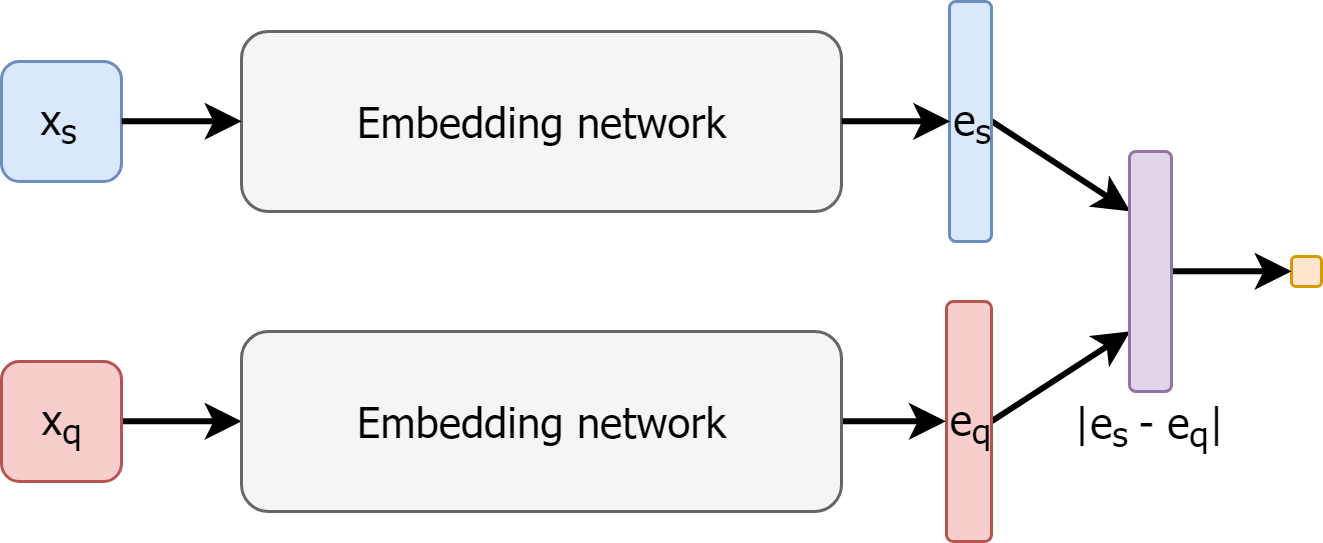
\includegraphics[width=9cm]{siamese}
 \caption{Overview of a siamese neural network}
 A network embeds support image $x_s$ and query image $x_q$ into $e_s$ and $e_q$, respectively. The absolute value of the difference of the embeddings is computed, then a fully connected layer outputs a single similarity value.
 \label{fig:siamese:2}
\end{figure}
The above-described technique is a \emph{mostly} data-driven approach for image similarity (we'll see a fully data-driven approach when discussing \textit{Relation Network} below) however this is an incomplete description of a one-shot image classification system. The novel aspect of this work is that while training, the system's task is solely image similarity, with targets of 1 when the image pair are from the same class, and 0 otherwise. When performing classification, this similarity operation is performed with pairs consisting of the query image and each example in the support set. The prediction is simply the class corresponding to the support image with which it had the highest similarity score. \par
This approach is very simple, achieves good results, and is well studied -- with siamese networks having been in use since as early as 1993 \parencite{earlysiamese}. However the amount of forward-passes increases proportionate to the number of classes, which makes it a poor candidate for continuous learning. The approach also only considers one-shot learning, which prevents the system from learning from more than one image. Although not discussed in the research paper, there are some simple modifications that could somewhat resolve these problems. The embedding function is fixed once trained, meaning that embeddings could be stored instead of images to serve as examples of classes. This minimises the increase in computation as new classes are added and makes it a better option for continuous learning. As for the limitation to one-shot learning, the system could easily be extended to allow for multiple examples per class, with the correct class being the one that receives the most "votes" across all examples. \par
Even with the aforementioned modifications mitigating some issues in applying this to continuous learning, some problems still persist. Although adding new classes is as simple as acquiring an image, there is no guarantee that the new classes come from the same data-distribution as what the model was trained on. The embedding network could then perform poorly and therefore damage the model's ability to accurately compute the similarity for these new classes. \par

\subsubsection{Matching Networks for One Shot Learning}
The work by Vinyals et. al. \parencite{matching} focuses on a problem encountered with previous works -- simple embedding functions work on a per-image basis, not taking into account the similarity between support classes. This is addressed by creating \emph{full context embeddings}, using an LSTM to compute $emb(x_i,S)$ for $x_i \in S$ where $S$ is the support set of images. These embeddings are then stored in external memory as in a memory network. Image queries are performed by using an LSTM as an attention mechanism over the stored embeddings and taking the class that received the greatest attention. Having full context embeddings allows the network to generalise to previously-unseen data distributions for new classes. \par
This solution is similar to model based meta-learning, but is more likely considered a metric based approach as the class prediction is made as a function of similarity to embedded support images. The one-shot results yielded by this technique are good, but in considering an extension to continuous learning we encounter obstacles. The size of memory needs to scale proportionate to the number of classes, and the LSTM embedding/attention mechanism is rather complex. \par

\subsubsection{Prototypical Networks for Few-Shot Learning}
The work by Snell et. al. \parencite{prototypical} proposes a simplified approach to metric based few-shot learning, while simultaneously considering the preservation of class examples without storing the actual images. Simply put, the concept is to compute a \emph{prototypical} embedding for each of the classes, and use this to perform queries. \par
The learnt embedding function is used to embed support examples, and the mean of the support embeddings is considered the ``prototype'' for that class. Query images are embedded in the same way, and the nearest prototype is used as the class prediction. Despite being a very simple approach, this achieved better results than aforementioned works and is quite performant, owing to the fact that a single embedding vector can be used to represent an entire class and doesn't need to be fed through the network again. This seems to be a good contender when considering the continuous learning domain, but a problem encountered is that the dimensionality of the embeddings may quickly become too small, resulting in embedding collisions; retraining of the network would be required to increase the capacity of the embeddings. \par

\subsubsection{Learning to Compare: Relation Network for Few-Shot Learning}
Sung et. al. \parencite{relationnet} identify that a weakness in metric based few-shot learning strategies lies in the fact that the distance/similarity calculation is pre-determined -- hand-engineered. They propose a solution with an entirely data-driven similarity module, and that allows for the classification between an arbitrary number of classes. \par
The network consists of two simple modules (see figure \ref{fig:relation-net:1})
\begin{itemize}
 \item\textbf{Embedding module}: A sequence of convolutional layers that produces a 3-dimensional feature map per image.
 \item\textbf{Relation module}: Given a pair of feature maps -- one each for a support image and query image -- concatenates them and applies a sequence of convolutional layers. Two fully-connected layers at the end of this module transform the output to be a single value: a similarity score.
\end{itemize}
The model's predicted class is the class of the support image with which the query image had the greatest similarity score. This approach allows the relation module to learn a -- possibly complex -- technique for calculating the similarity between a pair of images, rather than imposing a human understanding of similarity/distance. \par
\begin{figure}[h]
 \centering
 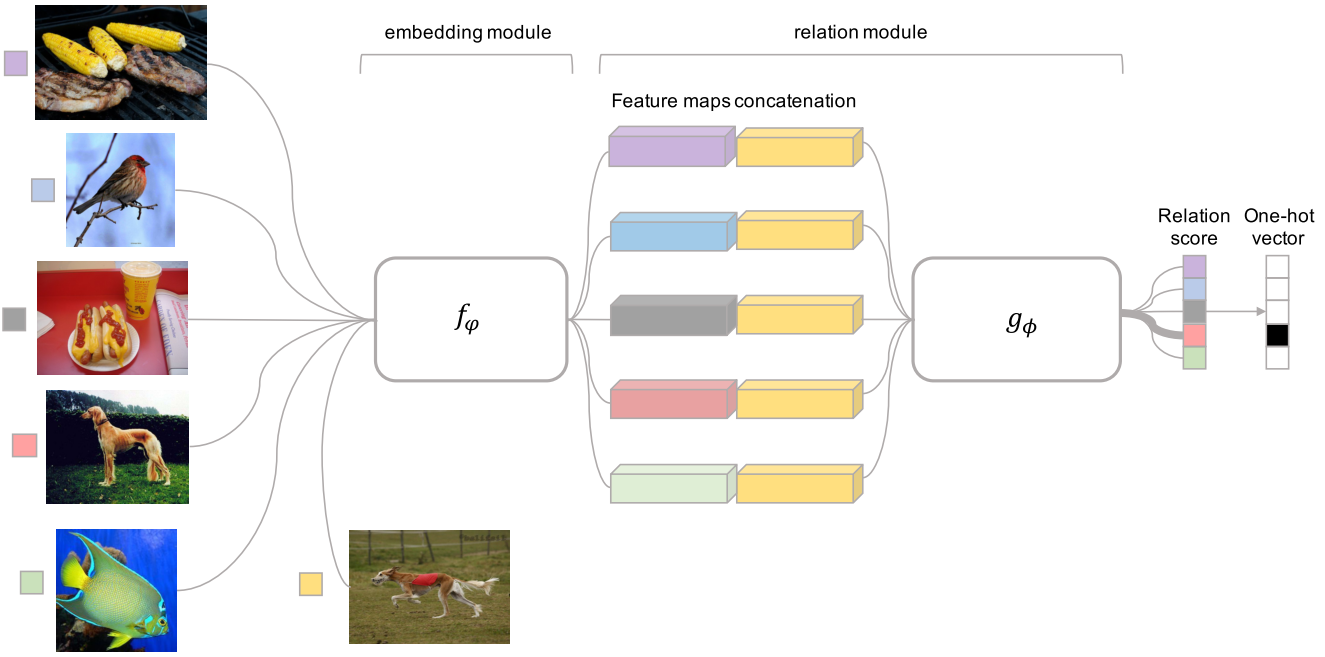
\includegraphics[width=14cm]{relationnet}
 \caption{Overview of Relation Network}
 The embedding module produces 3d feature maps for each support and query images, then each combination of (support, query) embedding pairs are further processed by the relation module to produce a relation score per pair. The predicted class is the maximum of these scores.
 \label{fig:relation-net:1}
\end{figure}
This incredibly simple solution achieves -- as of this writing -- the best results of any one-shot/few-shot techniques and is very easy to implement. However as with most metric-based approaches, Relation Network doesn't scale well as the number of classes increase, as a forward pass through the relation module needs to occur for every class and query image pair. This very quickly becomes a performance bottle-neck, and may be preventative for a many-class, high-resolution dataset. \newline \newline
The solutions presented in this section are generally quite simple to implement, but have problems with scaling to a large number of classes, as they require computing and comparing embedded representations for each query. This makes metric based methods an unappealing choice for continuous learning tasks, where the number of classes is -- by definition -- going to increase throughout the life of the system. \par

\subsection{Optimization Based} \label{related-meta-opt:1}
Optimization based solutions perform few-shot meta-learning by either learning an update rule which is substituted in place of a standard optimizer; or by learning an initial set of weights which are optimal for rapid improvement from few gradient steps. A major advantage of this technique over model based and metric based approaches is that a ready-to-go classifier is obtained after presenting the new class-examples, meaning that the model's computational complexity doesn't scale so dramatically with more classes. \par

\subsubsection{Optimization as a Model for Few-Shot Learning}
The work of Ravi et. al. \parencite{oaamffsl} identifies that the gradient descent update rule of a neural network (equation \ref{update:1}) resembles the cell-state update rule for an LSTM (equation \ref{update:2}), and considers that a standard optimizer could be replaced by an LSTM. Their approach proposes a meta-learner consisting of an instance of a shared-weight LSTM per parameter in the base-learner, such that each parameter is tracked by an LSTM with its own cell-state. A conscious decision is made to share the same weights between each instance, so as to minimize the overhead in tracking a large number of parameters. \par
\begin{align} \label{update:1}
 \theta_{t} = \theta_{t-1}-\alpha_{t}\Delta_{\theta_{t-1}}\mathcal{L}
\end{align}
\begin{align} \label{update:2}
 c_{t} = f_{t}\odot c_{t-1}+\i_{t}\odot \tilde{c}_t
\end{align}
The results garnered make this an impressive and powerful system, but not without its caveats. The training of LSTMs is notoriously tricky -- this paper mentions several specific hyper-parameters and design choices made to obtain such results. As such, difficulties would likely be encountered when applying the technique to different architectures or problem domains. \par
A limiting design aspect of this approach is that there is no communication between parameter LSTMs. The meta-learner's gradient updates are a function of only that specific parameter's history, therefore never allowing the meta-learner to have a ``global view'' of the model's weights or gradients. An ideal solution would allow for the modelling of relationships between parameters. \par

\subsubsection{Learned Optimizers that Scale and Generalize}
Following on from \parencite{oaamffsl}, Wichrowska et. al. \parencite{lotsag} also apply RNNs to the task of optimization in the few-shot learning domain, but allow interactions between parameters of the network by using a layered RNN structure (see figure \ref{fig:optimizer-that-scale:1}). This gives the meta-learner a better understanding of the loss-surface, and therefore the capacity to perform more informed gradient updates. Throughout the training of the meta-learner, a good initialisation for the collection of base-learners is implicitly learnt. They also implement several other improvements inspired by modern optimizers, which shall be briefly covered here as they are of interest for the problem in chapter \ref{problem-definition}.
The implemented features inspired by optimization literature are:
\begin{itemize}
 \item\textbf{Attention and Nesterov Momentum}: Nesterov Momentum (section \ref{nesterov}) computes gradients at future positions. Similarly they use RNN attention mechanisms to explore the loss surface ahead of the current parameter position.
 \item\textbf{Momentum on multiple time-scales}: By providing the optimizer with exponential moving averages of the gradients on several time-scales, the meta-learner has access to information about how rapidly the gradient is changing and about the degree of noise in the gradient.
 \item\textbf{Dynamic input scaling}: They provide the meta-learner with multiple metrics involving the scale of weights and gradients, thereby aiding the optimizer in becoming invariant to parameter scale.
 \item\textbf{Decomposition of output into direction and step-length}: They separate the optimizer's outputs into direction and step-length, and give it no access to the learning rate so it is forced to learn from the history of gradients, instead of memorising successful learning rates.
\end{itemize}
\begin{figure}[h]
 \centering
 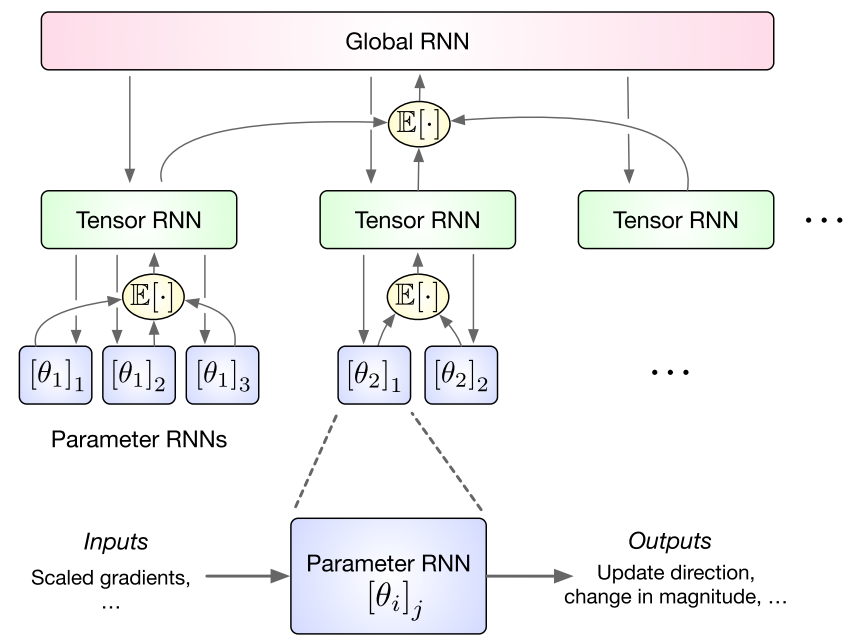
\includegraphics[width=10cm]{scalearchitecture}
 \caption{Learned Optimizers that Scale and Generalize architecture}
 The system utilizes three levels of RNNs, with shared weights between instances at each. Tensor and Global RNN instances receive the average latent state from the layer below, and pass down their outputs.
 \label{fig:optimizer-that-scale:1}
\end{figure}
Their experiments boast incredibly strong results, showing that -- unlike any prior methods -- this technique generalises to different problem domains, activation functions, architectures, and layer types; all previously unseen. This impressive feat is attributed to not only the layered RNN architecture, but likely the large number of aforementioned added features. Due to this complexity, this is a challenging system to re-implement and put to practice elsewhere. \par

\subsubsection{Model-Agnostic Meta-Learning for Fast Adaptation of Deep Networks}
The previous optimization-based meta-learning solutions primarily target the training of a network, but don't focus heavily on obtaining a good initial set of parameters. The approach by Finn et. al. \parencite{maml} called \emph{MAML} specifically addresses this, with the meta-learning process directly optimizing for initial parameters which can be rapidly re-trained to learn new tasks (see figure \ref{fig:maml-params:1}). There is no separate meta-learner, meaning that this technique is model-agnostic and can even be applied to different machine-learning optimization problems such as reinforcement learning. It only requires that the system is parametrized by some parameters $\bm{\theta}$, and that the loss function is smooth-enough in those parameters for gradient-based learning.
\begin{figure}[h]
 \centering
 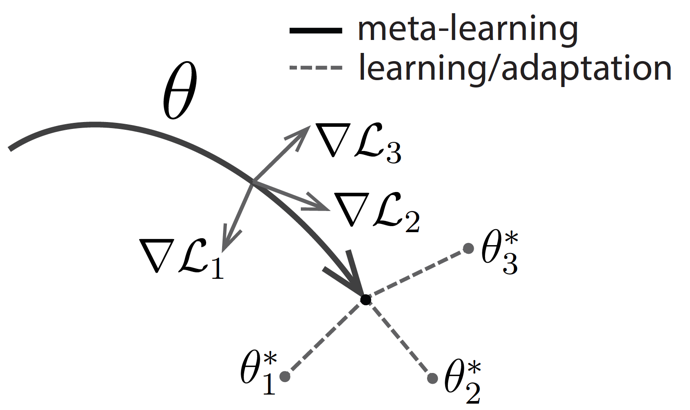
\includegraphics[width=6.5cm]{mamlparams}
 \caption{MAML optimization overview}
 MAML optimizes for parameters that can quickly adapt when shown new tasks. Here the new task optimal parameters are indicated by $\theta^*_i$
 \label{fig:maml-params:1}
\end{figure}
The meta-learning aspect of this approach is entirely in the training algorithm (see figure \ref{fig:maml-algo:1}), with the model initialized with random weights $\theta$. MAML computes adapted parameters from each task's training set, and temporarily stores the weights $\theta'_i$ per task:
\begin{align}
 \theta'_i = \theta - \alpha \Delta_{\theta} \mathcal{L}_{T_{i}}(f\theta)
\end{align}
Where $\alpha$ is a learning rate, $\mathcal{L}$ is a loss function, $f_\theta$ is a model parametrized by $\theta$, and $T_i$ is the $i$th task.
The meta-learner objective is then to minimize the loss jointly for the updated weights and parameters using the test-set of each respective task:
\begin{align}
 \min_\theta
 \sum_{T_i} \mathcal{L}_{T_{i}}(f_{\theta'_i}) =
 \sum_{T_i}\mathcal{L}_{T_{i}}(f_{\theta-\alpha\Delta_\theta\mathcal{L}_{T_{i}}(f_\theta)}) \label{eqn:maml}
\end{align}
The parameters of the model are then updated using gradient-descent, computing gradients for the loss computed in equation \ref{eqn:maml}:
\begin{align}
 \theta \gets \theta - \beta\Delta_\theta \sum_{T_i} \mathcal{L}_{T_{i}}(f_{\theta'_i}) \label{eqn:maml2}
\end{align}
Although techniques which meta-learn an update rule may intuitively be more efficacious, research \parencite{universality} has shown that there is no loss of representational power when solely optimizing the initial parameters. The same research also showed that learning the initial parameters in this way is extremely resilient to over-fitting on small datasets. The MAML algorithm yields very impressive results, with applicability to domains as varied as robotic control, reinforcement learning and computer vision. The technique allows rapid adaptation to unseen tasks, and is truly model-agnostic. The computation of equation \ref{eqn:maml2} is costly however, as it requires the calculation of second-order derivatives; it is desired to have a simpler technique in terms of computational complexity and implementation, as few libraries directly support second-derivatives. \par
\begin{figure}[h]
 \centering
 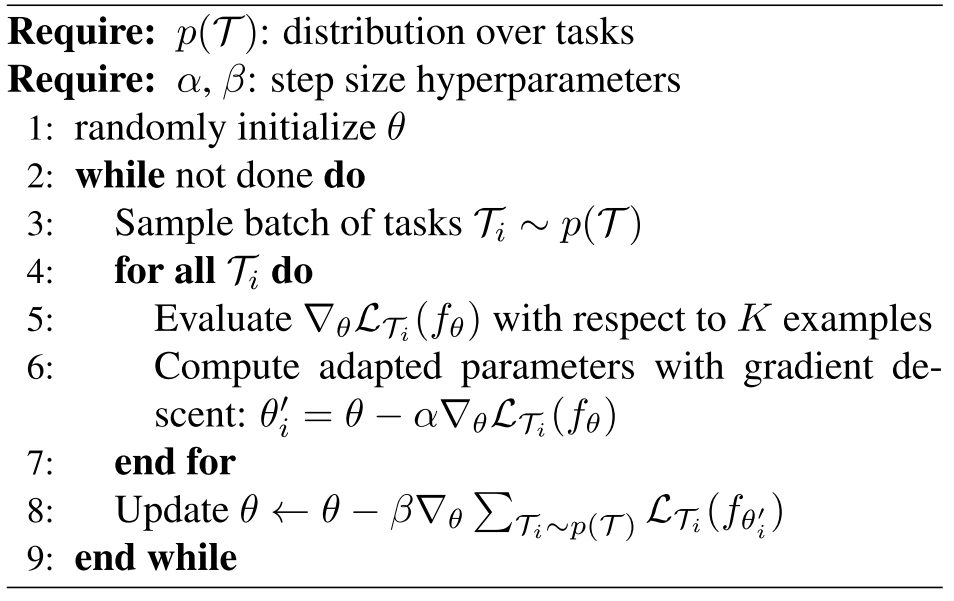
\includegraphics[width=9cm]{mamlalgo}
 \caption{MAML training algorithm}
 MAML computes adapted parameters from each task's training set (lines 5-6) then optimizes the model's parameters with the loss of each task's test set (line 8).
 \label{fig:maml-algo:1}
\end{figure}

\subsubsection{Reptile: a Scalable Metalearning Algorithm}
Nichol and Schulman \parencite{reptile} sought to remove the second derivative used in MAML, and replace it with a simpler mechanism with their development of Reptile. Reptile optimizes for parameters which can rapidly adapt to new tasks, using a simpler and more performant approach. \par
Reptile simply computes and temporarily stores updated weights $W_i$ for each task $T_i$ in a batch. The update applied to the parameters is a down-scaled gradient step in the direction of the sum all of them. Reptile effectively performs gradient descent in the direction of a number of tasks at once, without over-fitting to any of them.
\begin{figure}[h]
 \centering
 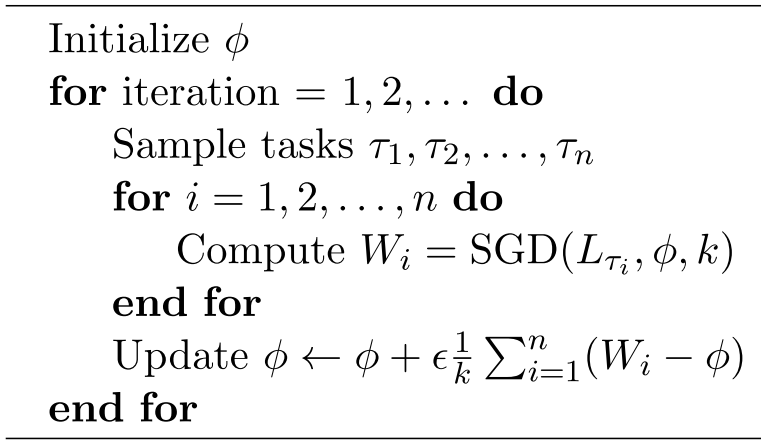
\includegraphics[width=6cm]{reptilealgo}
 \caption{Reptile training algorithm}
 Reptile computes updated weights per task, then performs a gradient step in the combined direction of all of them.
 \label{fig:reptile-algo:1}
\end{figure}
The results yielded by Reptile are similar to those of MAML, and provide a far-simpler implementation and better computational efficiency. Reptile has the same applicability as MAML, meaning it can be applied to essentially any model/task which can be optimized via gradient descent.


\section{Continuous Learning} \label{related-cont-learning:1}
Continuous learning techniques vary vastly, mainly as there is no general consensus as to what the task actually is, with the only agreement being that it is a system that can learn throughout a "lifetime", and retains information about previously learnt tasks. The works discussed in this section apply very different approaches to varying tasks, with most being partially inapplicable to real-world situations.

\subsubsection{Learning to Learn with Backpropagation of Hebbian Plasticity}
As already reviewed in section \ref{related-meta-modl:1}, the application of Hebbian plasticity to continuous learning developed by Miconi et. al. \parencite{ltlwbohb} is sensible, but limited ongoing as the model's internal representation never changes. This results in a fixed-capacity network which is highly dependant on the initial training. An ideal system would allow for parameters to change throughout the lifetime of the model to consolidate knowledge, and to learn new feature representations.

\subsubsection{Learning Without Forgetting}
A very literal approach to continuous learning, Li et. al. \parencite{lwf} attempt to mitigate catastrophic interference by considering the base model's responses to new classes of input images as targets. They do so by augmenting the model and adding a new "output head" (see figure \ref{fig:lwf:1}) for each new collection of classes introduced to the model. When training the model on these new classes, the pre-existing output heads' predicted probability distribution is recorded, and this is included in the loss calculation. \newline
\begin{figure}[h]
 \centering
 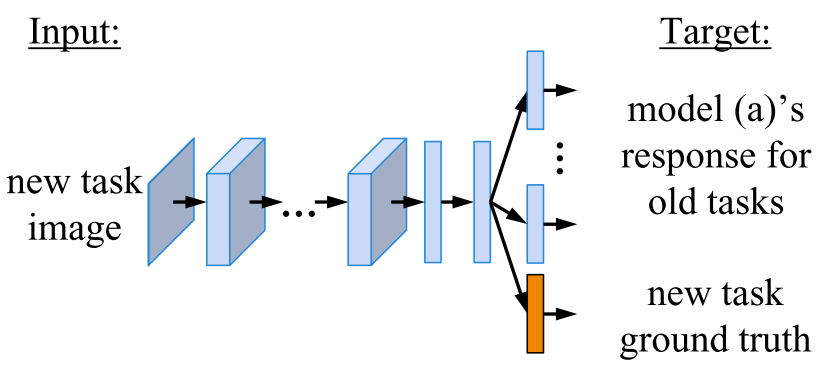
\includegraphics[width=8cm]{lwfarchitecture}
 \caption{Learning Without Forgetting architecture}
 A new output head (orange) is added for each batch of new classes. The model's predicted class probability distribution over the old classes is recorded and incorporated into the loss function.
 \label{fig:lwf:1}
\end{figure}
They utilize a loss function developed by Hinton et. al \parencite{distillation} which was designed to distil the information in a neural network; the original purpose was to compress knowledge into a smaller neural network. The loss for Learning Without Forgetting (LwF) is separated into two parts: $\mathcal{L}_{old}$ dealing with the pre-existing output heads' collective class distributions $\bm{y}_o$, and $\mathcal{L}_{new}$ dealing with the new output head's class distribution $\bm{y}_n$. Cross-entropy (equation \ref{eqn:lwf:1}) is used for the new output head, and distillation loss (equation \ref{eqn:lwf:2}) for all pre-existing heads. \par
\begin{align} \label{eqn:lwf:1}
 \mathcal{L}_{new}(\bm{y}_n,\hat{\bm{y}}_n) = -\bm{y}_n \cdot \text{log } \bm{\hat{y}}_n
\end{align}
\begin{align} \label{eqn:lwf:2}
 \mathcal{L}_{old}(\bm{y}_o,\hat{\bm{y}}_o) = -\sum_{i=1}^{l}\big( {y'}_{o}^{(i)} \cdot \text{log } \hat{y'}_o^{(i)}\big)
\end{align}
Where $\bm{\hat{y}}_n$ is the one-hot target over the new classes, $\bm{\hat{y}}_o$ is the recorded probability distribution, and $\hat{y'}_n^{(i)}$ and ${y'}_{o}^{(i)}$ are the targets and predictions over the old classes with weights increased for smaller probabilities. The training process is sensitive, so they perform a "warm-up stage" where only the parameters in the new head are trained, before training with the full loss function end-to-end. \par
While a simple and elegant approach, they produced mixed results. LwF's performance on the new dataset is quite consistently better than its competitors, yet demonstrates arbitrarily better and worse resilience to catastrophic interference for the old dataset. This could be a result of the fact that as the technique is not meta-learnt; the training process never receives direct feedback on its performance on the original dataset. If a new dataset and old dataset are not very similar, there is nothing ensuring that the model retains an internal feature representation that is relevant to the old classes; this would lead to performance degradation over time. \par

\subsubsection{Overcoming Catastrophic Forgetting with Hard Attention to the Task}
Taking inspiration from neurology, Serr\'a et. al. \parencite{hat} devised an implementation of \emph{inhibitory synapses} -- a biological process which makes a neuron less likely to fire. They perform this by learning a task-based hard-attention mechanism (HaT), which masks the activations on a per-neuron basis. They perform a learnt embedding of the task description per layer, which acts as the gate for that layer. This teaches the network to learn sparse internal representations for each task, effectively reducing the required capacity within the network during training, and allowing for re-use of suitable feature representations. \par
Serr\'a et. al. claim to address catastrophic interference well, stating that their technique yields reductions of previous class knowledge loss of 45 - 80\%. There is potential for the application to meta-learning tasks, though this is unexplored as of yet. A core limitation to this work is that the tasks must align in their output format; that is, each of the tasks were strictly image classification between 10 classes. Adding additional classes to the model is unsupported, and as such, its applicability to real-world continuous learning is quite limited. \par

\subsubsection{Gradient Episodic Memory for Continual Learning}
Gradient Episodic Memory (GEM), proposed by Lopez-Paz et. al. \parencite{gem} considers storing examples in memory to mitigate catastrophic forgetting. They store and compute loss for the $m$ most recently-seen examples from each task, with a total memory budget of $M=mT$ for $T$ distinct tasks, evicting memories on a least-recently-used basis. Storing examples for "replay" is a long-established technique, and isn't a true method of knowledge retention. The model would quickly over-fit if the parameters were to be repeatedly optimized for everything in memory, seeing each example $m+1$ times before eviction. GEM side-steps this by instead minimising the loss with the constraint that loss for old examples cannot increase. \par
\begin{figure}[h]
 \centering
 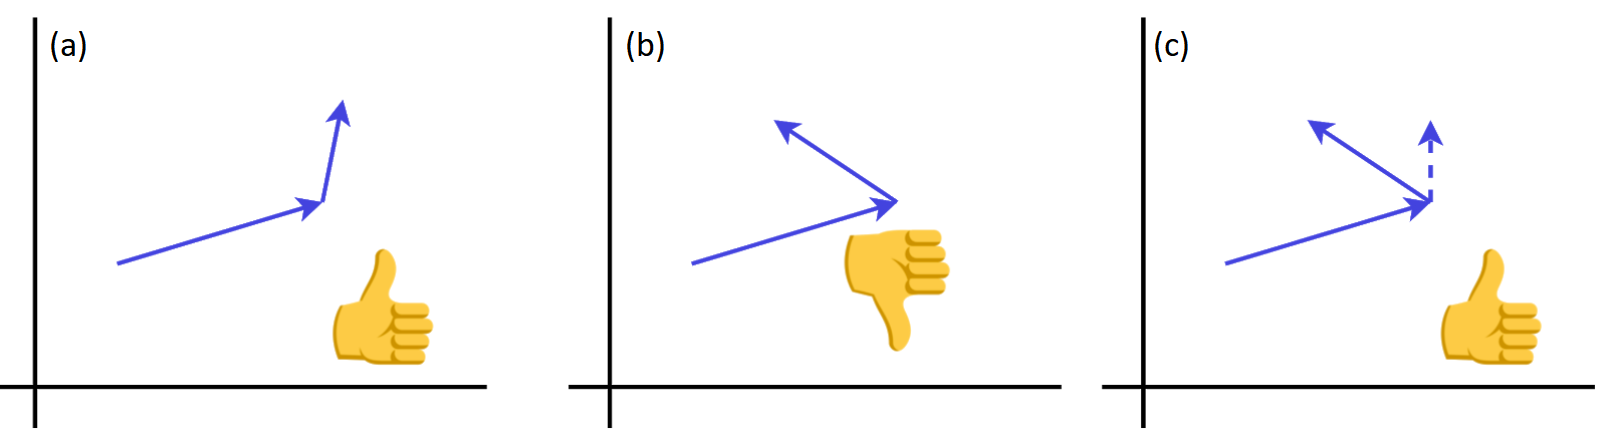
\includegraphics[width=11cm]{gem}
 \caption{GEM gradient proposal example}
 When gradients computed for new examples and memories agree (a), they are accepted; when they disagree (b), a new gradient is proposed (c) that satisfies the constraints.
 \label{fig:gem:1}
\end{figure}
Minimising with constraints is an unconventional technique, and is posed as a per-parameter vector-direction constraint. They first compute the gradient for each parameter for the given example, then similarly compute the gradient for each example stored in memory. If the direction of the proposed gradient step doesn't point in the same direction as the gradient computed from memory (figure \ref{fig:gem:1}), they adjust the update direction to satisfy both directions. This can be seen as not directly optimizing towards a loss minimum for the memories, but as never adjusting parameters away from this minimum. \par
This method demonstrates a strong reduction in catastrophic interference, but has two problems which cause the practicality of this method is questionable. It involves -- in a very literal sense -- storing old examples and replaying them, which goes against the idea of a true continuous learner and grows rapidly as the number of tasks increase. Secondly, this technique doesn't allow for a varied number of classes between classification tasks, which limits it to only tasks with the same output format. \par

\subsubsection{Learning to Accept New Classes without Training}
Hu Xu et. al. \parencite{l2ac} introduce a system with the name ``L2AC'' which -- while focused on continuous learning -- allows for zero-shot learning at the same time. In a manner similar to Prototypical Networks \parencite{prototypical}, they consider classification to be a similarity measure between the query example and a set of class exemplars. They only apply their approach to text-based classification, but the work can simply be translated to the image domain. \par
This work distinguishes between ``seen'' and ``unseen'' classes, whereas most other classification networks simply make predictions according to the class with the highest probability, regardless of the query example belonging to the known classes. However, what truly sets this work apart from Prototypical Networks and Relation Network \parencite{relationnet} is the introduction of a ``ranker'', which has the sole responsibility of finding the top-k most similar seen class examples before performing the costly comparison (figure \ref{fig:l2ac:1}). \par
\begin{figure}[h]
	\centering
	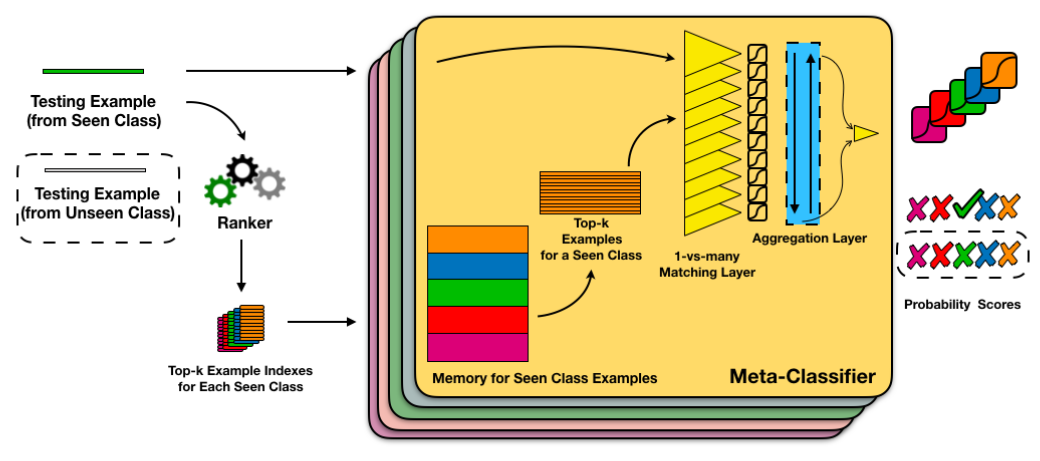
\includegraphics[width=14cm]{l2ac}
	\caption{L2AC system architecture}
	A query example is embedded, and the ranker finds the top-\textit{k} most similar embedded class exemplars. The meta-classifier computes the similarity between these \textit{k} examples and the query example, with the class-prediction being the highest probability class, if it is above a confidence threshold.
	\label{fig:l2ac:1}
\end{figure}
For this text-based task, they utilise a pre-trained bidirectional-LSTM for encoding, and the ranker is simply the cosine similarity between the example and all stored examples. While this is an overly simple technique for classification, for the task of selecting the top-k, it more than suffices. The actual classification occurs in the Meta-Classifier, which has a ``1-vs-many Matching Layer''. This consists of the concatenation of the two examples' absolute difference, and element-wise summation to produce a ``similarity space'' vector. This new vector is passed through two fully-connected layers and a sigmoid function, to produce a scalar similarity score. An aggregation layer is used to produce a single class prediction, and the query example is considered to be from an unseen class if there is no class probability $> 0.5$. \par
As noted, this technique is similar to previously discussed metric-based meta-learners, but has the added benefit that costly comparisons need not be made between all classes. As with all other metric-based solutions, it still has the undesirable property of needing to retain class examples for future usage. Due to the reduced number of comparisons, and the fact that only example embeddings need to be stored, this effect is minimised, but still present.

\subsubsection{Overcoming Catastrophic Forgetting}
Kirkpatrick et. al. \parencite{ewc} propose a solution for continuous learning by designing a loss function that ties parameters to a space in which the model performed well on a previous task. They introduce an algorithm referred to as Elastic Weight Consolidation (EWC), which slows down learning on weights based on how important they are to previously seen tasks, and gives learning trajectories to maintain optimal performance (figure \ref{fig:ewc:1}). They essentially seek to find a set of good parameters for a new task that is close to good parameters for previous tasks. \par
\begin{figure}[h]
 \centering
 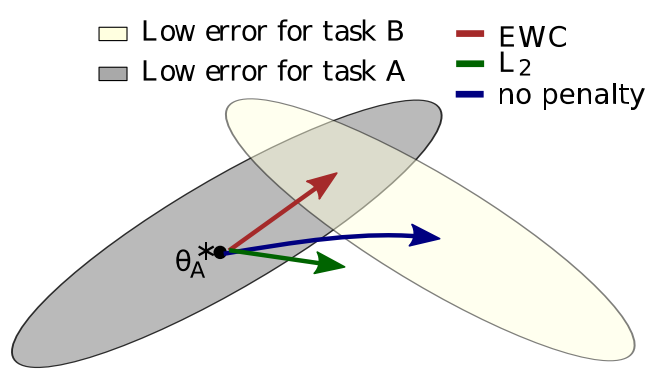
\includegraphics[width=7cm]{ewc}
 \caption{Elastic Weight Consolidation parameter updates}
 EWC causes training trajectories which maintain performance on old tasks.
 \label{fig:ewc:1}
\end{figure}
They use a Fischer information matrix $F$, which is an analytical tool for estimating the importance of the parameters $\bm{\theta}$. They then use this to weight the loss of a quadratic function which constrains the parameters to stay in the region of good performance for previous tasks $A$. As the function is quadratic, the parameters are anchored to $\theta_{A,i}^*$ as by a spring, forcing the trajectory shown in figure \ref{fig:ewc:1}. The loss function then, is:
\begin{align}
 \mathcal{L}(\theta) = \mathcal{L}_B(\theta) + \sum_{i} \frac{\lambda}{2} F_i (\theta_i - \theta_{A,i}^*)^2
\end{align}
where $\mathcal{L}_B$ is the loss for a new task, and the sum is the loss of the parameters, which elastically constrain the parameters to a space near good performance on task $A$. \par
Given that the solution can be implemented by simply computing a Fischer information matrix and amending the loss function, it's a highly attractive technique. That being said, although it's generalisable to most parametrized machine-learning systems, as with most other techniques it doesn't allow for a varied number of classification categories between tasks.

\section{Summary} \label{works:summary}
In this chapter we have discussed works related to the domains of few-shot and continuous learning, and considered their feasibility to be extended to the joint-task of few-shot continuous learning. A summary of the results are shown in table \ref{fig:table:1}, where we see that there is no ideal technique. \par
As expected, the methods that designed for few-shot learning are consistently applicable to few-shot tasks; we do see, however, that none of the approaches could be considered entirely applicable to continuous learning. The reasons vary between techniques, ranging from entirely incompatible to functional to a limited capacity. \par
Surprisingly, the continuous learning works are largely incompatible with our desired subset of continuous learning -- that is, the addition of an arbitrary number of classes. Most don't allow arbitrary numbers of classes to be added, with the only compatible method (Learning without Forgetting) having no capacity for few-shot learning. \par
The problem discovered then, is that not only has continuous learning with an arbitrary number of added classes not been thoroughly studied, but that there is a large gap in pre-existing works which combine few-shot and continuous learning. This leaves us with a rather un-addressed -- yet important -- class of machine-learning problems. Having recognised the shortcomings of other approaches, in the next chapter we will propose a solution which attempts to address the outlined concerns. \par
\begin{table}[h]
 \centering
 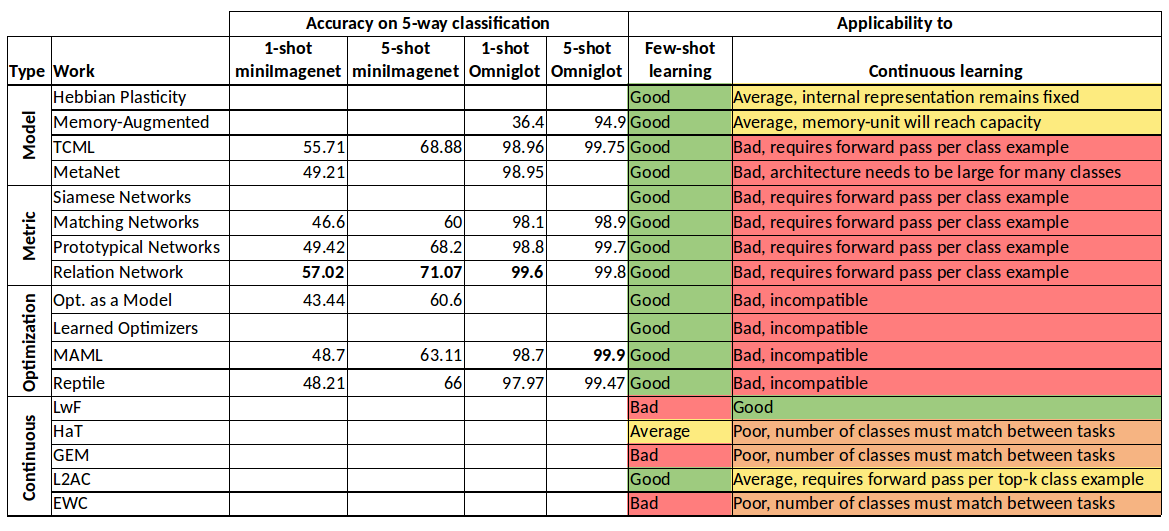
\includegraphics[width=17cm]{table}
 \caption{Related works comparison}
 \label{fig:table:1}
 Validation-set accuracy and feasibility of application to few-shot and continuous learning for related works. Entries are empty where no results are reported.
\end{table}


\chapter{Problem Definition} \label{problem-definition}
The task is \textit{model augmentation} -- to take a model which has been trained to classify $n$ classes $\bm{X}_S = {X_S^1, X_S^2, ..., X_S^n}$, and using only the model's weights and a \emph{small} number of examples from $m$ disjoint classes $\bm{X}_T = {X_T^1, X_T^2, ..., X_T^m}$, produce a model which can perform well (measured using the equations in section \ref{metrics}) on the combined set of classes $\bm{X}_S \cup \bm{X}_T$. For example, if we have a source model with the classes $\bm{X}_S = \lbrace apple, banana, carrot \rbrace$, augmenting the model with $\bm{X}_T = \lbrace date, elderberry \rbrace$ would result in a target model with the ability to classify between classes $\bm{X}_S \cup \bm{X}_T = \lbrace apple, banana, carrot, date, elderberry \rbrace$.
Furthermore, the ideal solution would be repeatable, such that a model can be continuously extended throughout its lifetime. \par
While the relatively recent resurgence of meta-learning techniques has prompted much research in few-shot and continuous learning, no previous works attempt this task precisely. This is largely because there is much to be done in each of these individual domains, with state-of-the-art results surpassed on a very regular basis. That being said, the efficacy of meta-learning techniques is beginning to reach a limit, meaning that more novel applications are able to be considered.	\par
The previous work that is nearest to the proposed task is \textit{Learning without Forgetting}\parencite{lwf} -- the fact that the loss function incorporates the persistence of old knowledge means that it is a strong contender. As noted however, this technique results in a separate set of class predictors for each added task, meaning that the domain of the input images must be known prior to performing inference. Furthermore, there is much to be gained by applying a meta-learnt system to the task, as carrying information between models allows for more generalised knowledge. An additional benefit is that an episodic learning schema provides opportunity to perform one-shot training. \par

\section{Key Terminology}
\textit{Source classes} are the set of classes on which a \textit{source model} has been pre-trained without meta-learning. Similarly, a \textit{target model} is produced by extending a source model's classification ability to also include a set of \textit{target classes} -- a disjoint set of classes to those that the source model was trained on. \\
\textit{Pre-training} refers to the procedure by which a source model is prepared. The \textit{meta-learner} is the system which performs the transformation of a source model into a target model.

\section{Metrics} \label{metrics}
The performance of a Meta-Learner is measured by two components: the accuracy of the target model on the target classes, and the accuracy of the target model on the source classes. The former is a measure of how much the model learns about the target classes; the latter a measure of how much the model retains accuracy on the source classes. Instead of considering the precision in terms of their absolute value, we will instead compute the difference between target model and source model precision. Concretely, for a collection of images, a model will produce a number of correct (C) and incorrect (I) predictions. We can therefore compute the precision for a given model $\bm{\theta}$ on images $\bm{x}$ as in equation \ref{eqn:evaluation:1}.
\begin{align} \label{eqn:evaluation:1}
Precision(\bm{\theta}, \bm{x}) &= \frac{C}{C+I}
\end{align}
To compute the relative improvement or deterioration of performance of a model, we need to compute the difference in precision between a source model and corresponding target model. It is not possible to measure the source model's performance on the target classes directly however, as it is in the problem definition that the source model has never seen the target images. In this case, we use the source model's performance on the source classes as a proxy for initial performance. We define and use two metrics for assessment of a Meta-Learner's performance, retention and acquisition.\par
\subsubsection{Retention}
A measure of the Meta-Learner's success in retaining performance on the source classes, where a score of 0 indicates that the Meta-Learner discarded all prior knowledge, a score of 1 indicates that the Meta-Learner perfectly retained all prior knowledge, and a score $>1$ indicates that the Meta-Learner improved performance on the source classes. While a score $>1$ is unlikely, it is not strictly impossible, as it is possible that the Meta-Learner learns additional information other than what's given explicitly as inputs as a result of seeing a wide variety of models during training. The equation for retention is 
\begin{align}
Ret(\bm{\theta}, \bm{x}) &= \frac{Precision(\bm{\theta}_T, \bm{x}_S)}{ Precision(\bm{\theta}_S, \bm{x}_S)}
\end{align}

\subsubsection{Acquisition}
A measure of the Meta-Learner's success in learning to predict for the target classes, where a score of 0 indicates that the Meta-Learner failed to learn anything, a score of 1 indicates that the Meta-Learner learned to predict for the target classes with the same accuracy as it performed on the source classes before training, and a score $>1$ indicates that the Meta-Learner performed better on the target classes than it did on the source classes before training.
\begin{align}
Acq(\bm{\theta}, \bm{x}) &= \frac{Precision(\bm{\theta}_T, \bm{x}_T)}{ Precision(\bm{\theta}_S, \bm{x}_S)}
\end{align}

\section{Analysis of Naive Solutions}
To highlight the difficulty of model augmentation we will first analyse the shortcomings of some naive solutions. This in turn motivates our use of the meta-learning approach to solve this problem. \\
The typical approach to augmenting a model is to simply add new weights, and train on target class examples -- this most closely resembles transfer learning, as described in section \ref{transfer-learning}. To that end, three experiments were performed to investigate the effects of catastrophic forgetting in a standard neural network (see figure \ref{fig:dir:1}). Each of the experiments began with the same model pre-trained for 50-way classification, then extended to perform 60-way classification by adding 10 additional classes. We perform these experiments using a 4-layer fully-convolutional neural network, with the Adam optimizer on the CIFAR100 dataset. Full details are given in section \ref{datasets}. \par
The first of the experiments (figure \ref{fig:dir:1}a) was to continue training the model with no steps taken to mitigate catastrophic forgetting -- simply adding new output classes and training. This resulted in almost instantaneous catastrophic forgetting, with the accuracy on the source classes rapidly approaching zero. \par
The second experiment (figure \ref{fig:dir:1}b) was to continue training in a similar manner, but disallowing any changes to the weights that provide predictions for the source classes. This affected no change to the results, as the target class head could very quickly grow the magnitude of the prediction probabilities to ``out-weigh'' the predictions of the source class prediction head. \par
The third experiment (figure \ref{fig:dir:1}c) attempted a more drastic technique to minimise catastrophic forgetting, by disallowing changes to any part of the model's weights except for those in the target class output head. As seen in the figure, catastrophic forgetting took a much longer time to cause a problem, but regardless still occurred. \par
\begin{figure}[!h]
 \centering
 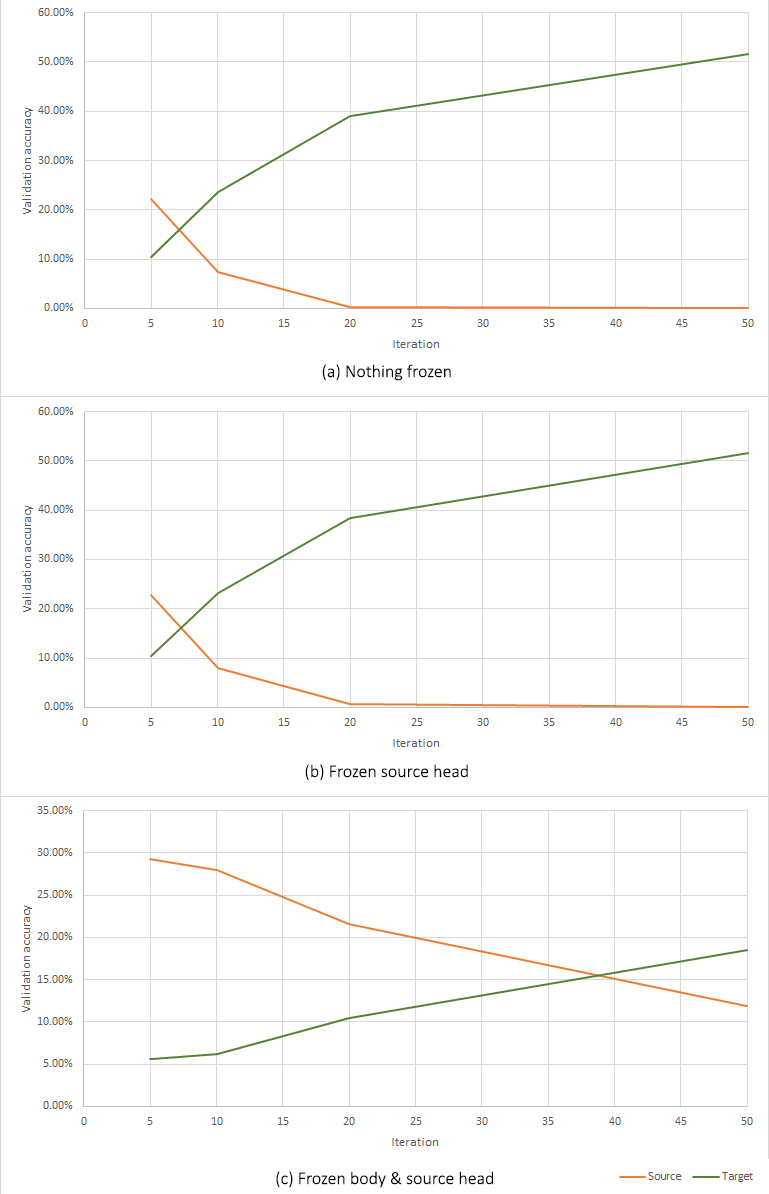
\includegraphics[width=10cm]{dir-1}
 \caption{Validation accuracy with catastrophic forgetting}
 (a) All weights in the network allowed to change; (b) only the model's body and target head allowed to change; (c) only the target head allowed to change.
 \label{fig:dir:1}
\end{figure}
These results demonstrate that a more sophisticated solution is required if we are to extend a network as desired. We wish to therefore devise a system that can take an already-training classification model and a set of few target class example images, and produce a new model with the capacity to classify both old and new classes. \par
We quickly come up against a few major hurdles.The major hurdles then, are:
\subsubsection{Optimisation take no consideration for pre-existing knowledge}
As previously discussed, catastrophic forgetting occurs due to the optimizer minimising the loss for the given batch of examples by adjusting the model's weights, with nothing constraining the updates such that they preserve the network's existing internal feature representations. The challenge then, is to devise a way of applying gradients such that the knowledge embedded in the network is retained. The meta-learning setup could facilitate this, as by viewing the adaptation of the model itself as a learnable problem could allow for the implicit understanding of what ``embedded knowledge'' looks like within a model's weights.
\subsubsection{Gradients don't necessarily represent the whole dataset}
Using a small batch of examples for computing an update gradient causes similar problems to the previous point, in that the gradient only represents the best update \textit{given the current batch of examples}. Therefore, the traditional optimisation technique of applying an update consisting of a scaled step in the negative of the gradient is limited by way of the gradient itself not having enough information to bring the model to the true optimum parametrisation. The task is to leverage more information than is encoded in the gradient, just as other few-shot learning techniques do. In addition, the internal feature representation of a neural network is typically underutilised, as demonstrated by \parencite{hat} where having a learnt attention over the model allowed for a sparse internal representation. This implies that there is sufficient capacity in an average model to be extended to additional tasks. Furthermore, the meta-learning setup we wish to employ should once again allow us to see the parametrisation and re-parametrisation of the model as a learnable problem, giving us the capacity to learn a generalised representation of the internal characteristics of a trained model, and compute updates within that context. \par

\section{Inputs and Outputs}
As discussed, the meta-learner must itself perform the updates to a model with respect to a set of target class example images. The inputs to the meta-learner must therefore be a set of model parameters and either the target class examples, or gradients computed using those images as inputs to the model. For these works, we have chosen the latter. \par
As the desired outcome is to produce a new set of parameters for a model, we have a few options for what type of outputs we desire. The meta-learner can directly produce new weights for a model, the set of updates to apply to the pre-existing model, or a number of variations on the two. These will be discussed later in chapter \ref{methodology} where we consider the effects of each option. \par
A  view of the meta-learning system architecture appears in figure \ref{fig:metalearnersimple:1}, the details of which are discussed in section \ref{commonalities}.

\begin{figure}[!h]
 \centering
 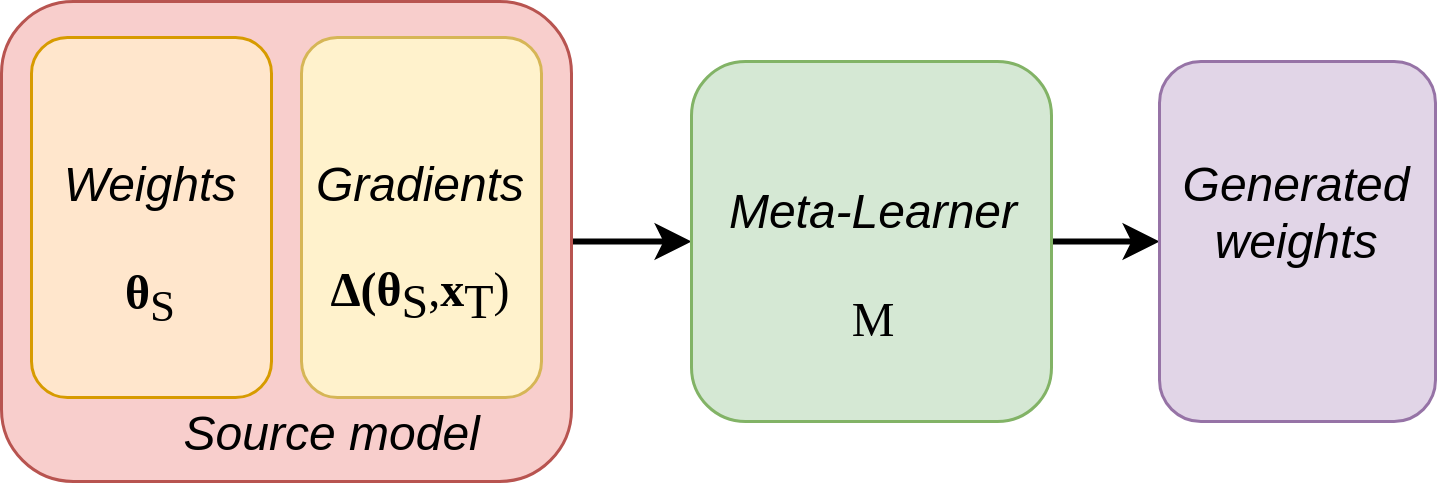
\includegraphics[width=10cm]{ml-highlevel-overview}
 \caption{High-level meta-learner overview}
 The meta-learner takes as inputs the source model weights, the gradients of the target class images with respect to the source model, and outputs a generated set of weights.
 \label{fig:metalearnersimple:1}
\end{figure}

\section{Summary}
In this chapter we have discussed the general structure of our problem, and given a brief overview of what role the meta-learner must take in this task. It is clear at this point that the task is far from trivial, and requires overcoming multiple obstacles which appear to be inherent to gradient-based optimisation methods. \par
We will now discuss the specific setup for the task, and the technique by which we perform each experiment. \\


\chapter{Methodology} \label{methodology}
Convolutions have proven useful for computer vision, as local information is sufficient to form an understanding of the relationships between pixel values. We present a novel solution that applies a convolutional network to the parameters of a neural network, suggesting that a local view of a network's layers is sufficient to form an understanding of the relationships between weights. We build a Meta-Learner which convolves over the weights and gradients of a network and produce a new set of weights as its outputs. Our solution merges the tasks of few-shot learning and continuous learning -- an intersection that is largely unexplored -- adjusting the parameters of a neural network using few examples from a new set of classes such that it can classify these new classes also. \par
Although the task is to take an arbitrary $N_{S}$-way classifier and extend that to be a $(N_{S}+N_{T})$-way classifier, we will focus on a specific number of classes, where $N_{S} = N_{T} = 5$; so as to minimise the amount of training time. \par
We present a solution which uses standard neural network components typically used for computer vision to rapidly re-parametrise a classification model to be performant on an extended set of classes. At a high level, our algorithm computes gradients for a model using examples from a new set of classes, takes these gradients and the weights they pertain to as inputs and produces a set of ideal updates to apply to the model for the combined classification task. Many variants of the solution are explored in section \ref{approaches}, but we will begin by describing the general design of the solution, which forms the basis of all experiments. \par

\section{Source Model Setup} \label{commonalities}

\subsubsection{Pre-Training} \label{pre-training}
At its core, the theme of the task is to extend the knowledge in an already-trained network. We must therefore pre-train a collection of "source models" which act as the inputs to the meta-learner -- each of which need be trained on a unique class subset. \\
For a dataset consisting of $C=100$ classes, there are ${C\choose N_S} = 75,287,520$ such unique subsets of size $N_S$. This is far more models than we wish to train, so we instead employ a simpler technique for subdividing the dataset into $C-N_S$ subsets: 
\begin{align}
	\bm{X}_i = \lbrace X_i, X_{i+1}, ..., X_{i+N_S-1} \rbrace, i \in[1, C-N_S] 
\end{align}
These class subsets are grouped into meta-train and meta-test sets with no overlap in classes across the two, with $\sim$20\% in the meta-test set. For our case of 100 classes, this results in 71 meta-train models (classes 1-75) and 20 meta-test models (classes 76-100). Each of these models is trained to convergence on the 5-way classification task, with care taken to not overfit to the relatively small training set - see figure \ref{fig:pre-training-acc:1} for the accuracy during this pre-training phase. \\

\begin{figure}[h!]
	\centering
	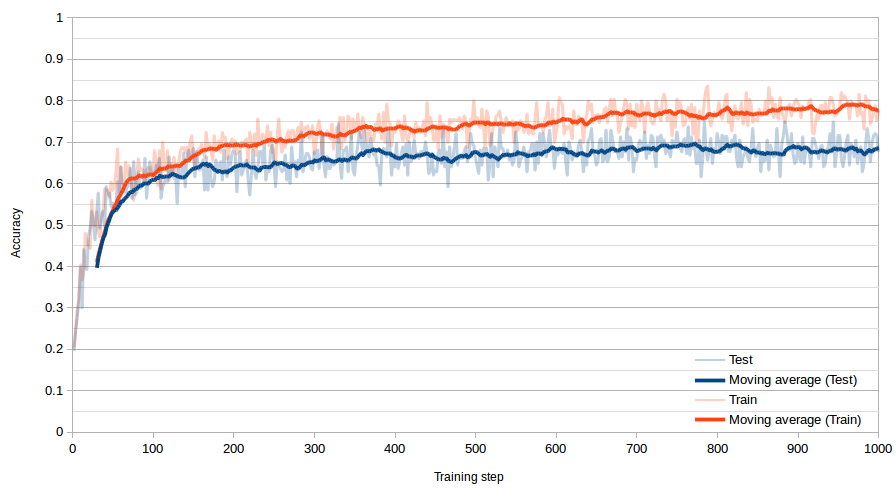
\includegraphics[width=16cm]{pre-training-acc}
	\caption{Pre-training accuracy on 5-way CIFAR100}
	\label{fig:pre-training-acc:1}
	Values reported are the mean of 10 models
\end{figure}

\subsubsection{Two-Stage Pre-Training}
For certain variations on the algorithm (section \ref{approaches}), there is a necessity to perform two-stage pre-training. Two-stage training results in a collection of models that each have identical feature-extractors (bodies), but different classification heads. For the bodies to be identical across each source model, we must pre-train the models on a collection of classes that are completely distinct from those that we wish to use in our meta-learning tasks. If this consideration weren't taken, the source models may have knowledge leveraged from target classes ahead of the meta-learning -- thereby breaking the conditions of the experiments. \par
The first phase is to train a model on a set of classes completely disjoint from those to be used in meta-learning task, as a means of learning a good feature-extractor. In cases where there were insufficient classes to perform this stage, the dataset with most similar features was chosen. \par
The second phase is to ``focus-train'' these models, where the heads are trained on the source classes with the bodies remaining frozen. \par


\subsubsection{Model Architecture}
The architecture of all source/target models is the same between experiments (figure \ref{fig:model-arch:1}), and are a small variation on a fairly standard meta-learning architecture. The primary difference being that we have chosen not to include biases in any of our layers, in an attempt to simplify the embedding/un-embedding discussed in section \ref{meta-learner-sub}. In addition to this, the model is fully-convolutional, and as such the predicted class probabilities are simply the maximum value in each channel of the output head.

\begin{figure}[h!]
	\centering
	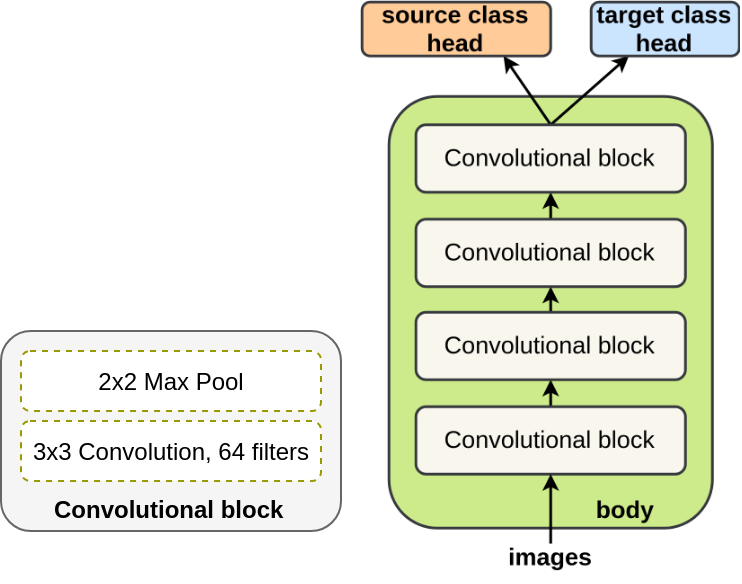
\includegraphics[width=8cm]{model-arch}
	\caption{Source/target model architecture}
	\label{fig:model-arch:1}
\end{figure}


\section{Meta-Learner} \label{meta-learner-sub}
The algorithm consists primarily of a meta-learner $M$, which takes the weights of a source model $\theta_S$, a set of target class images $\bm{x}_T$, and produces a set of updates $\Delta_M$ as below:

	\begin{align}
	\Delta_M = M(\bm{\theta}_S, \bm{x}_T)
	\end{align}

We will first discuss the structure of a meta-learner, what occurs during a single training ``episode'', then will further clarify the episode-based training procedure. At a high-level, the meta-learner architecture (figure \ref{fig:ml:3}) consists of four stages:
\begin{itemize}
	\item \textbf{Gradient calculation} - Gradients are calculated for the source model using target images.
	\item \textbf{Embedding} - The weights and associated gradients for each layer are separately mapped to a fixed size matrix then stacked to form a 3d matrix with a depth of 2 -- maintaining separation between weights and gradients. The mapping is performed by ``pseudo-convolutions'' -- sliding fully-connected layers across the source-model weights, mapping each dimension to a fixed-size.
	\item \textbf{Encoding and Decoding} - The weights and gradients are convolved over and down-sampled to produce a spatially-compressed representation, which is then convolved over further and up-sampled to return to the original spatial-dimensions. This output representation will only have a depth of 1, as we desire a single update value per-parameter.
	\item \textbf{Unembedding} - The decoded representation is un-embedded to match the shapes of the input weights.
\end{itemize}
\begin{figure}[h!]
	\centering
	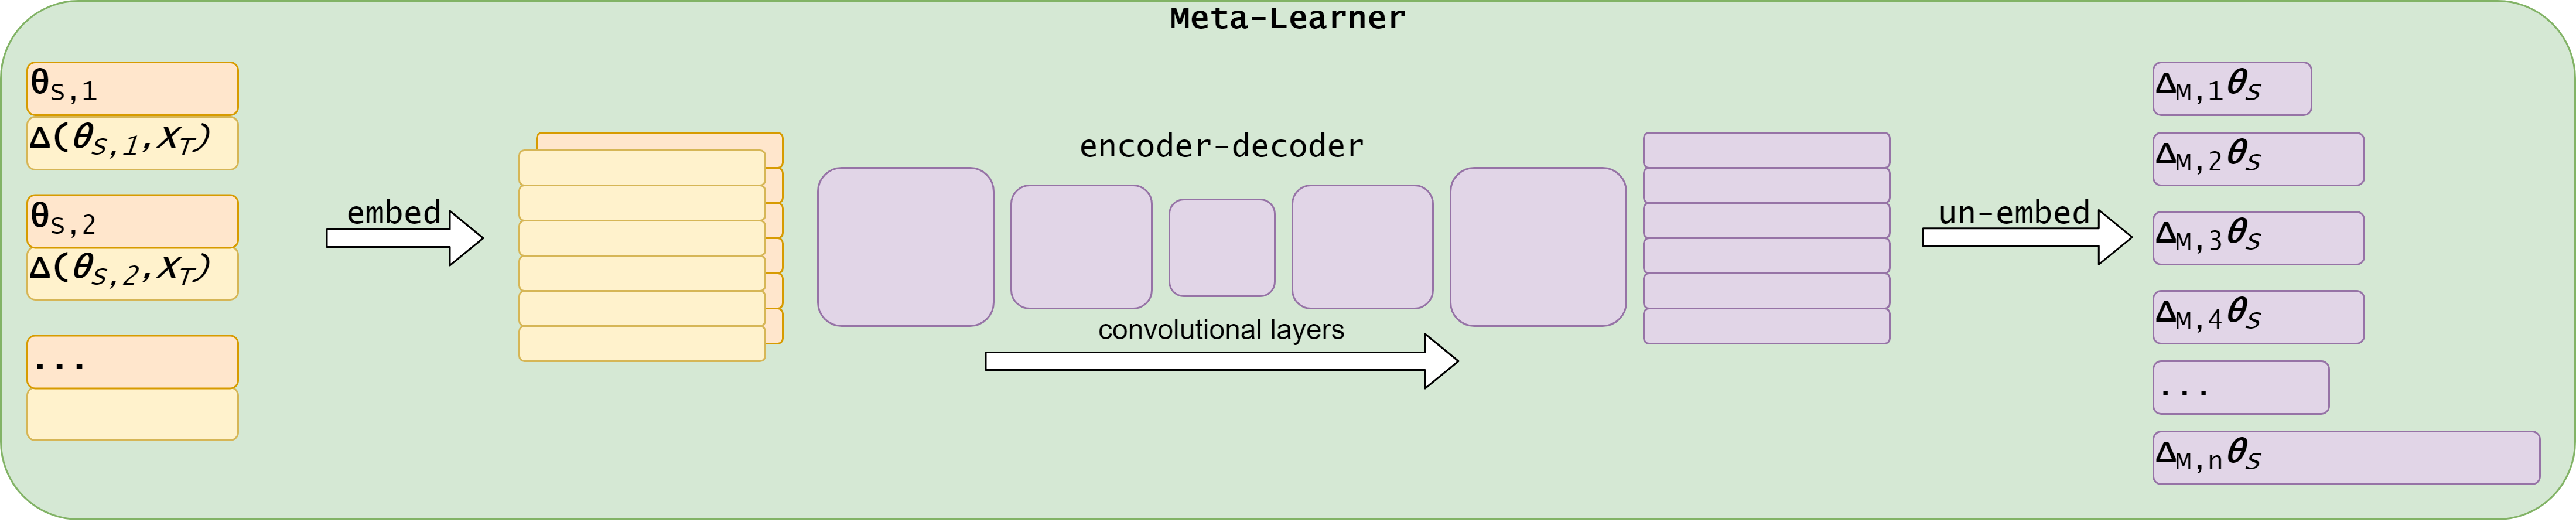
\includegraphics[width=17cm]{metalearnerarchitecture}
	\caption{Meta learner architecture overview}
	\label{fig:ml:3}
	Gradients and weights are embedded, encoded, decoded and unembedded to their original shape.
\end{figure}
The target model is then produced by applying the model outputs as parameter updates to the source model -- some alternatives to a simple gradient update are discussed in section \ref{approaches}. \par
Even the best adaptive optimizers (section \ref{optimizers:1}) consider only per-parameter information, without seeing the relationship between weights within even the same layer. The intuition for the encoder-decoder based approach is that as the weights and gradients are convolved and the spatial size of the features decreased, the meta-learner gains a more global perspective. We work with the assumption that gaining a larger perspective of parameter relationships is vital in performing a single, successful weight update. The encoder-decoder structure therefore allows for a large spatial view into the features to produce meaningful updates. It is this contextual information allows for the dramatic changes to parameters necessary for few-shot learning. \par
Our solution is considered ``optimization based'', as we are dealing directly with the weights and gradients themselves. This is the only practical solution, as model based and metric based options impose restrictions on the model architecture - which is something we aim to minimise. \par




\subsection{Model Preparation}
Each source model $\bm{\theta}_S$ consists of a body and a source-class output head -- pre-trained to perform well on the related source classes. This model does not yet have output weights for the target classes, mapping features to probability predictions. Therefore, the models must be extended prior to entering the meta-learner. \par
We do so by adding a new set of $N_T$ output channels to the model's existing head. The initialisation of these new weights are drawn from a truncated normal distribution (values which follow a normal distribution, but where those with magnitude greater than 2 standard deviations from the mean are dropped and re-picked), with the mean and standard deviation selected to match the distribution of the source class output head. The weights in the source model were populated in the same manner during the pre-training procedure. Some alternative initialisation schemes are explored later, in section \ref{approaches}. It is only at this stage, when the model has the correct number of output classes, can it be given to the meta-learner. \par

\subsection{Inputs}
The inputs to the meta-learner must be not only the model's weights, but also some gradients computed with relation to the target classes. We consider only the 5-shot task, such that we can gain good insight into the distribution of each class -- moreso than the 1-shot task. As such, using 5 examples from each of our target classes, we compute the loss between the model's 1predictions and the labels using mean-squared error (section \ref{loss:1}), and perform back-propagation through the model to compute the gradients. \par
We now have a set of gradients - one for each weight in the source model, including the target class output head. At this point, all source class information is embedded in the model's weights, and that all target class information is embedded in the related gradients. We consider that this is sufficient to learn a good, generalised update to the source model to produce a high-performing target model.

\begin{figure}[h!]
	\centering
	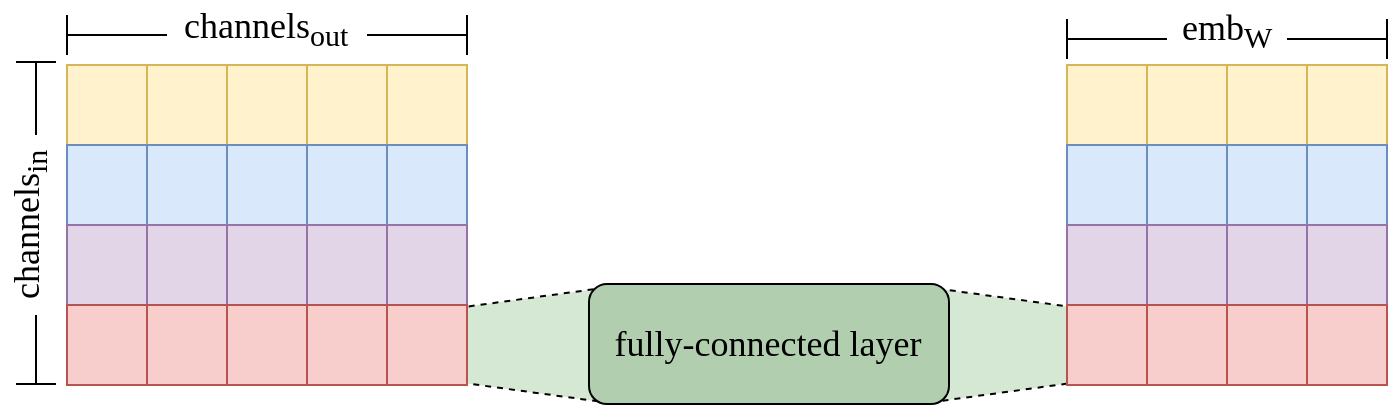
\includegraphics[width=12cm]{embedding}
	\caption{2D tensor embedding}
	\label{fig:embedding:1}
	A fully-connected layer slides along the height of a 2-dimensional tensor, mapping to a fixed-width. The same function is applied to the resultant tensor's height, mapping to a fixed-height. \textit{Unembedding operates in the same manner, but mapping from the embedded shape back to the original.}
\end{figure}
\subsection{Embedding}
As we wish to minimise restrictions on model architecture, we must somehow reshape the weights and gradients such that it is largely architecture independent. We do so by performing an embedding on the weights in each layer. The implementation used in experiments don't allow for the source model having biases or fully-connected layers, though we do give that some consideration in (section \ref{future-works}). \par
The layers in a neural network consist of a varying number of weights, including convolutional layers. The weights of a convolutional layer are of shape
\begin{align}
	(kernel_{H}, kernel_{W}, channels_{in}, channels_{out})
\end{align}
So a 2D convolutional layer with a 3x3 kernel, from 16 input channels to 32 output channels has weights shaped $(3, 3, 16, 32)$. Although we can restrict the kernel shape to ensure consistency across two of the dimensions, it is unavoidable that the last two dimensions will be of arbitrary size. Our embedding function (figure \ref{fig:embedding:1}) takes care of this, by mapping the two last channels to a fixed shape. \par
We do so by first combining the first two dimensions of the weights, to obtain a 3d tensor shaped
\begin{align}
	(kernel_{H}*kernel_{W}, channels_{in}, channels_{out})
\end{align}
We now consider the first dimension to be a ``batch dimension'' and apply the same embedding function to each element along that dimension. The operation works by first compressing along the 2\textsuperscript{nd} dimension, then the 3\textsuperscript{rd}. \par
To do so, we construct fully-connected layers as required, mapping $channels_{in} \rightarrow emb_H$, where $emb_H$ is a hyperparameter specifying the height of the embedded weight. Similarly, we construct fully-connected layers mapping $channels_{out} \rightarrow emb_W$, for the embedded width. These fully-connected layers slide along the 2\textsuperscript{nd} and 3\textsuperscript{rd} dimensions in succession, to obtain a new tensor shaped
\begin{align}
(kernel_{H}*kernel_{W}, emb_H, emb_W)
\end{align}
which is a consistently-sized tensor for all layers when the kernel shape is fixed. We then flatten this tensor to provide a one-dimensional tensor shaped 
\begin{align}
(kernel_{H}*kernel_{W}*emb_H*emb_W)
\end{align}
It is important to flatten the tensor in this way, such that every layer in a neural network provides the same 1-dimensional embedding. Repeating this embedding function across all weights of a neural network results in a tensor shaped 
\begin{align}
(n_{layers}, kernel_{H}*kernel_{W}*emb_H*emb_W)
\end{align}
where the size variability comes solely from the number of layers in a network. \par
The fully-connected layers in this embedding function utilise weight-sharing where possible, lazily creating new layers only as required. As the gradients of the source model are of the same shape as the weights, this procedure is repeated for those also, resulting in maximum weight-sharing to facilitate the learning of a good embedding function. \par

\subsection{Encoding/Decoding}
As discussed, our embedding function maps the entirety of a neural network's weights into a 2-dimensional tensor. Performing this same embedding operation on the gradients of the source model and stacking the results gives a 3D tensor, with a last dimension of size 2. This shape is similar to that of a typical image, with the number of ``colour channels'' in this case equal to two. \par
A typical architecture for computer-vision neural networks is an \textit{encoder-decoder}, where the input image is convolved over, and has its spatial dimensions increased while increasing its depth dimension to produce an encoded representation of the knowledge held in the image. The inverse of this architecture is applied to the encoded image, decreasing the depth dimension while increasing the spatial dimensions. We apply this type of encoder-decoder network (figure \ref{fig:ml:3}, middle) to our embedded network weights, in order to produce a set of embedded model updates. The decoder output spatial dimensions are set to match the input, but the number of output channels is not fixed. This allows us to experiment with having the encoder-decoder learn to produce more than just the raw weight updates -- which are explored in section \ref{approaches}. \par
Just as local information is sufficient to form an understanding of the relationships between pixel values in typical computer vision encoder-decoders, we work with the hypothesis that local weight/gradient information is sufficient to learn good update rules. In addition, this fully-convolutional architecture allows for an arbitrarily-sized network, consisting of any size embeddings and any number of layers. This allows for the encoder-decoder to be used for source models of arbitrary structure. \par

\subsection{Unembedding}
The decoded updates are still in an embedded space, and don't match the dimensions of the weights and gradients that were input to the beginning of the Meta-Learner. At this stage we apply an unembedding function, which is the logical inverse of the embedding function (figure \ref{fig:embedding:1}) -- unembedding can be seen as a special case of embedding, where the embedded size matches the shapes of the inputs from earlier. It is worthwhile noting that although we make good use of shared weights in both the embedder and the unembedder, we don't allow weight-sharing between the two so as to not impose the same operation of both embedding and unembedding. Embedding and unembedding are not necessarily the same operation -- despite their similar nature -- as embedding typically is a technique for encoding into a more abstract representation, while unembedding is the reverse.

\section{Training Procedure}
As with other meta-learning setups we adopt an episodic training procedure, where images are seen from both the training and test set in a single episode. The procedure during meta-training and meta-testing works in the same way, but with each using a disjoint subset of classes as described in section \ref{pre-training} - pre-training. \par
The training procedure is outlined in figure \ref{fig:ml:2} and algorithm \ref{alg-episode}, but in its simplest form, consists of the following steps:
\begin{enumerate}
	\item Randomly sample a pre-trained source model $\bm{\theta}_S$, and add randomly initialised output weights.
	\item Randomly sample a set of target classes $\bm{X}_T$, not overlapping with the source-classes.
	\item Randomly sample training images $\bm{x}_{T,train}$ and test images $\bm{x}_{T,test}$ with classes $\bm{X}_T$.
	\item Generate weight updates $\bm{\Delta}_M = M(\bm{\theta}_S, \bm{x}_{T,train})$.
	\item Build target model by adding generated weight updates $\bm{\theta}_T = \bm{\theta}_S + \bm{\Delta}_M$.
	\item \textit{(meta-training only)} Perform backpropagation through meta-learner with examples from combined test sets $\bm{x}_{S,test} \cup \bm{x}_{T,test}$, thus optimising the generation of weight-updates.
\end{enumerate}
\begin{figure}[h!]
	\centering
	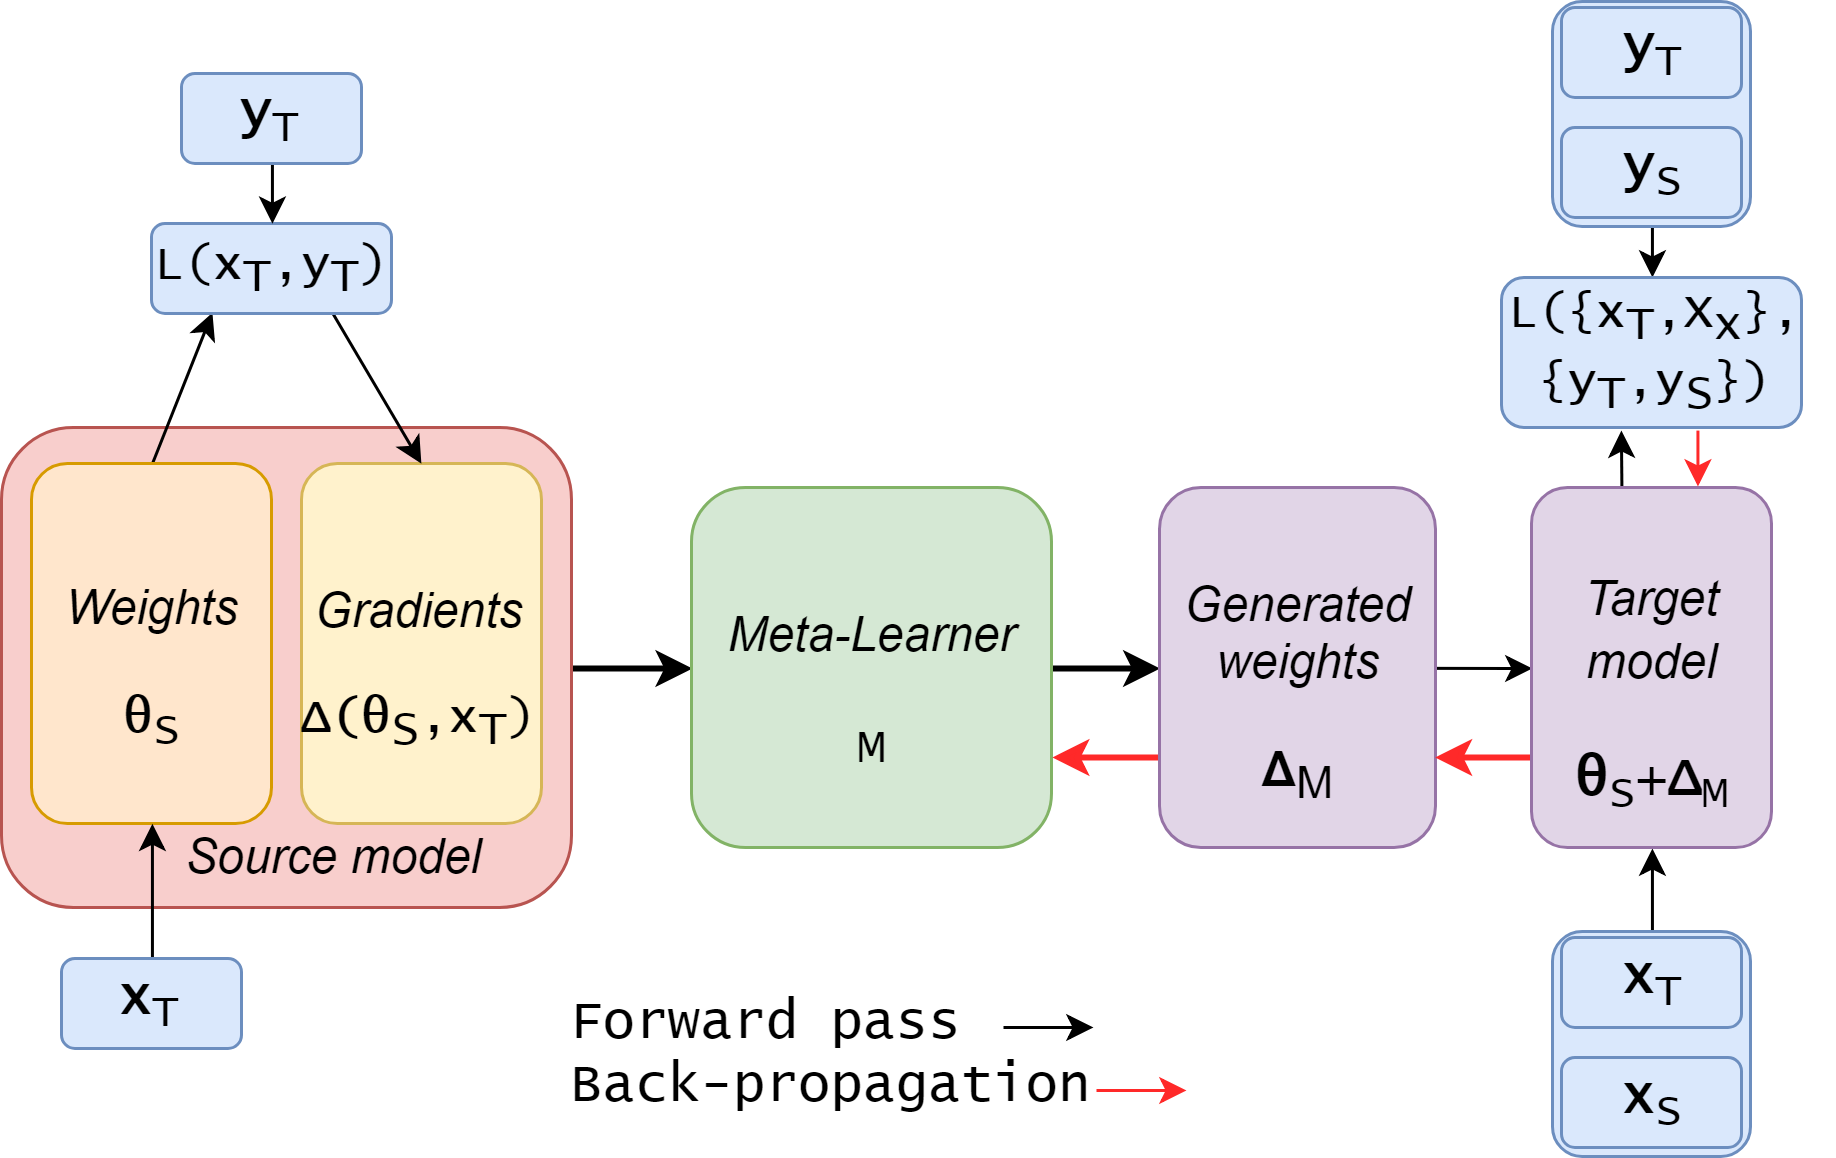
\includegraphics[width=11cm]{metalearneroverview}
	\caption{Meta learner training procedure}
	\label{fig:ml:2}
	The Meta-Learner takes source model weights and target example gradients as input, and produces a set of weight updates. This new model predicts for the source and target classes, and the error is backpropagated into the Meta-Learner. 
\end{figure}
As during each episode the Meta-Learner sees not only a different set of source and target classes and images but a different model, the Meta-Learner becomes invariant to these -- i.e. it doesn't depend on a specific  model, class set, or image distribution. This allows for meaningful knowledge to be obtained throughout training, thus maximising generalisation capability. \par

\begin{algorithm}[h!]
	\caption{Meta-Learner $K$-shot Training Episode}
	\label{alg-episode}
	\begin{algorithmic}[1]
		\Require{Meta-Learner $M$ consisting of weights $\bm{\theta}_M$}
		\Require{Source model $\bm{\theta}_S$, source classes $\bm{X}_S$, target classes $\bm{\theta}_T$}
		\Require{Model initialisation function $init$}
		\Require{Learning rate $\alpha$}
		\State Sample $K$ target class examples $\bm{x}_{T,train}$ per class in $\bm{X}_T$
		\State $\bm{\theta}_S \gets init(\bm{\theta}_S, \mathcal{N}(\mu, \sigma^2))$
		\Comment{Extend model with random weights}
		\State Evaluate $\nabla(\bm{\theta}_S,\bm{x}_T)$
		\Comment{Compute gradients using target images}
		\State $\bm{\Delta}_M \gets M(\bm{\theta}_S, \nabla(\bm{\theta}_S,\bm{x}_T))$
		\Comment{Meta-Learner generates weight updates}
		\State $\bm{\theta}_T \gets \bm{\theta}_S + \bm{\Delta}_M$
		\State Sample $K$ source class examples $\bm{x}_{S,test}$ per class in $\bm{X}_S$
		\State Sample $K$ target class examples $\bm{x}_{T,test}$ per class in $\bm{X}_T$
		\State $\bm{x}_{test} \gets \bm{x}_{S,test} \cup \bm{x}_{T,test}$
		\State Evaluate $\nabla(\bm{\theta}_M, \bm{x}_{test})$
		\Comment{Compute Meta-Learner gradients using test examples}
		\State {Update $\bm{\theta}_M \gets \bm{\theta}_M - \alpha \nabla(\bm{\theta}_M, \bm{x}_{test})$}
	\end{algorithmic}
\end{algorithm}

\section{Variants} \label{approaches}
With such a complex system, there are numerous design choices and opportunities for experimentation. We group these into four categories and explore each separately -- namely: \textit{dataset complexity}, \textit{weight initialisation}, \textit{meta-learner inputs} and \textit{meta-learner outputs}. Here we discuss the significance of each category, and describe the variants explored. \par

\subsection{Dataset Complexity}
As will be discussed in section \ref{results-chapter}, the complexity of the dataset play a role in the success of this algorithm. We explore this with three different datasets (described in section \ref{datasets}), each with varying degrees of success. This is a problem for future work (discussed in section \ref{future-works}), but suitably serves our purposes. \par

\subsection{Weight Initialisation} \label{weight-init}
Weight initialisation has long been considered of crucial importance with regards to the successful training of a neural network \parencite{heinit}\parencite{weightinit}. As such, consideration was given to the initialisation of the new weights used for target-class predictions. \par
The initialisation of a typical neural network strongly influences the model's performance, and this effect is amplified in a complex solution such as ours. It is important that -- at the very least -- the magnitude of the new weights is similar to the existing weights in the same layer; a large disparity between the scale of weights within the same layer typically introduces a disparity in the usage of features, where certain weights ``outvote'' others. It is common to employ $L_2$ weight regularisation in neural networks to enforce this property, but this is beyond the scope of our discussion. Due to the significance of weight initialisation, we experiment with the following alternative schemes:

\subsubsection{Random Initialisation}
Weights are randomly sampled from the same distribution from which the source model was initialised (algorithm \ref{random-init}) -- the most simplistic initialisation scheme.
\begin{algorithm}[h!]
	\label{alg:random-init}
	\caption{$init$ - Random Initialisation }
	\label{random-init}
	\begin{algorithmic}[1]
		\Require{Source model output head weights $\bm{\theta}_{S,n}$}
		\Require{Number of target classes $N_T$}
		\State Compute mean $\mu$ and standard-deviation $\sigma^2$ of $\bm{\theta}_{S,n}$
		\State Sample $N_T$ weights $\bm{\theta}'$ from truncated normal $\mathcal{N}(\mu, \sigma^2)$
		\State $\bm{\theta}_{S,n} \gets [~ \bm{\theta}_{S,n}~ ~ \bm{\theta}'~ ]$
		\Comment{Stack new weights with existing}
	\end{algorithmic}
\end{algorithm}

\subsubsection{Copy-Random Initialisation}
Weights are built as in \textit{Random Initialisation} once only, and re-used for all source models. The expectation is that the weights produced using random initialisation act as a source of noise for the Meta-Learner, resulting in a more complex task for the Meta-Learner to apply meaningful updates. Using a copy-random strategy should allow for the meta-learner to become accustomed to a random distribution, without needing to compensate for the differently sampled points during each episode.

\subsubsection{Copy Initialisation}
Weights are duplicated from the source output head into the target output head (algorithm \ref{copy-init}). Differences in number of source/target classes -- and the subsequent difference in number of weights in each head -- are resolved by repeating or slicing the weights as required. \par
It is expected that this technique will not yield especially good results, as the weights in the source-class output head are likely very specialised to specific relationships between features and class predictions. This sparsity introduces imbalance between weights, meaning that significantly different magnitude updates need be applied to weights depending on the original weight's scale.
\begin{algorithm}[h!]
	\caption{$init$ - Copy Initialisation }init
	\label{copy-init}
	\begin{algorithmic}[1]
		\Require{Source model output head weights $\bm{\theta}_{S,n}$}
		\Require{Number of target classes $N_T$}
		\State Copy $N_T$ weights $\bm{\theta}'$ from $\bm{\theta}_{S,n}$
		\Comment{Weights are repeated or removed if too few or too many}
		\State $\bm{\theta}_{S,n} \gets [~ \bm{\theta}_{S,n}~ ~ \bm{\theta}'~ ]$
		\Comment{Stack new weights with existing}
	\end{algorithmic}
\end{algorithm}

\subsection{Meta-Learner Inputs} \label{ml-inputs}
The algorithm description until this point has considered that the Meta-Learner will take the entirety of a neural network's weights and their related gradients as inputs; we explore the effects of only giving the final (output) layer weights as inputs, and maintaining the body of each model fixed. For this to be possible, the body of each source model must be identical, lest the Meta-Learner have an incomplete view of feature/class relationships. With the bodies identical and fixed, the Meta-Learner should be able to learn an implicit relationship between features in the body and classes in the output heads. It is in this case that we perform the two-phase pre-training as already described in section \ref{pre-training}.

\subsection{Meta-Learner Outputs}
Although the Meta-Learner is described as producing only a set of weight updates $\bm{\Delta}_M$, the encoder-decoder architecture allows us to produce a variable number of outputs per weight. We explore this by considering a few alternatives:

\subsubsection{Deltas}
The Meta-Learner only produces a delta (weight update) per weight, such that the update rule to produce a target model is (as shown earlier)
\begin{align}
\bm{\Delta}_M &= M(\bm{\theta}_S, \bm{x}_{T,train}) \\
\bm{\theta}_T &= \bm{\theta}_S + \bm{\Delta}_M \label{eqn-delta-updates}
\end{align}


\subsubsection{Gates and Deltas}
In addition to the delta, a gate in $[0, 1]$ is produced per weight, which -- much like an LSTM or memory network (sections \ref{lstm}, \ref{memory-nets:1}) -- dictates ``how much'' of the old weight should be kept. This allows the model to ``switch off'' weights if they serve little purpose in the target model. The update rule in this case becomes
\begin{align}
\bm{\Delta}_M, \bm{\sigma}_M &= M(\bm{\theta}_S, \bm{x}_{T,train}) \\
\bm{\theta}_T &= \bm{\sigma}_M \odot \bm{\theta}_S + \bm{\Delta}_M
\end{align}
where $\bm{\sigma}_M$ is the Meta-Learner's predicted gate value after being passed through a sigmoid activation layer.


\subsubsection{Gates and Tanh Deltas}
We also explore applying a non-linearity $tanh$ function to the deltas produced, as a way of forcing the new weights to be in the range of $[-1, 1]$. This is in essence a form of output normalisation, not allowing the Meta-Learner to produce very large-scale outputs. This results in an update rule of
\begin{align}
\bm{\Delta}_M, \bm{\sigma}_M &= M(\bm{\theta}_S, \bm{x}_{T,train}) \\
\bm{\theta}_T &= \bm{\sigma}_M \odot \bm{\theta}_S + tanh(\bm{\Delta}_M)
\end{align}


\section{Summary}
We have now described the techniques used to prepare our source models prior to meta-learning, and the base-methodology to train the Meta-Learner. Along with this we have selected a wide-variety of Meta-Learner variants with which we will experiment, and given reasonable support for their selection. We will now describe our experimental setup, including the datasets, software and hardware utilised in these experiments.


\chapter{Experimental Setup} \label{experimental-setup}
\section{Datasets} \label{datasets}
Our research requires that any dataset possesses a few properties: a large number of classes; small image resolution (for speed in training); and -- ideally -- consistent image features between classes, to allow for the transfer of learnt features to new classes. Each of the following datasets have these properties, along with their own benefits and detriments. We apply our meta-learning system to the first three of the following datasets, with varying degrees of success. \par

\subsection{Omniglot}
The Omniglot\parencite{omniglot} dataset is a collection of 1623 28x28 different handwritten characters from 50 alphabets, each with 20 examples drawn by different people (figure \ref{fig:omniglot:1}). The characters are black on a white background, and made up of relatively simple features. Due to the small number of examples per class, Omniglot is regularly used for few-shot learning experimentation\parencite{mlwtc}\parencite{matching}\parencite{prototypical}.

\begin{figure}[h]
	\centering
	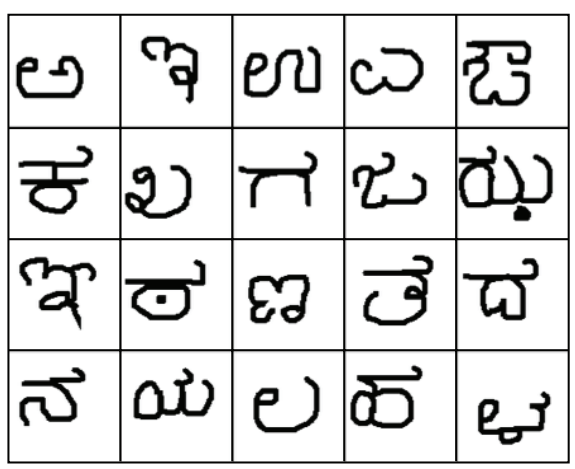
\includegraphics[width=5cm]{omniglot}
	\caption{Omniglot dataset images}
	A small selection of characters found in the Omniglot dataset.
	\label{fig:omniglot:1}
\end{figure}

\subsection{CIFAR100}
The CIFAR100\parencite{cifar100} dataset consists of 60,000 32x32 images in 100 classes with 600 images per class (figure \ref{fig:cifarexamples:1}). The small resolution of this dataset is beneficial for meta-learning, as it allows for relatively short training times and subsequently, rapid prototyping. The features found in CIFAR100 don't necessarily represent real-world image features very accurately however, as a lot of subtleties are lost in the resizing.
\begin{figure}[h!]
	\centering
	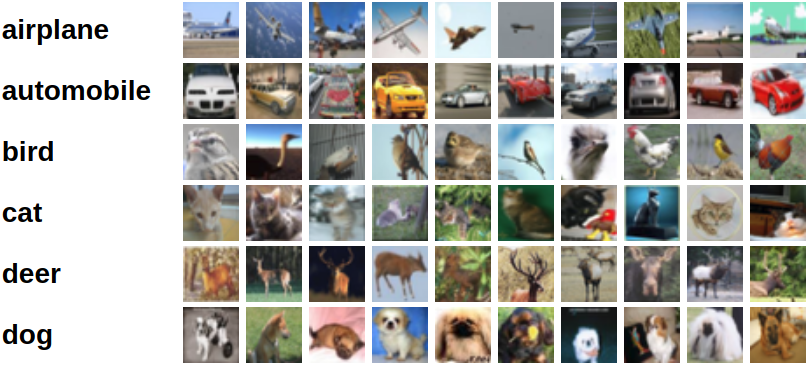
\includegraphics[width=12cm]{cifarexamples}
	\caption{CIFAR100 dataset images}
	Examples from 5 classes found in CIFAR100
	\label{fig:cifarexamples:1}
\end{figure}

\subsection{BLOCKS}
The BLOCKS dataset was created to provide a simpler collection of images than CIFAR100 to use for prototyping. It consists of 69,500 32x32 images in 139 classes with 500 images per class. Each class is a permutation of bright and dark colours in a 3x3 grid, with each example a random colour, scale and position on a black 32x32 image (figure \ref{fig:blocks:1}). \par
Unlike the other two datasets, BLOCKS is completely synthetic, with no attempt to mimic real-life image distributions. The lack of complex image features lessens the burden of feature-learning from the neural network, as the relationships that form the objects in this dataset don't go much further than a simple combination of edges and corners. Although the dataset is inarguably simpler than the other two, it still remains sufficiently complex to demonstrate the inference capacity of a neural network, without resulting in over-fitting to the training set.

\begin{figure}[h]
	\centering
	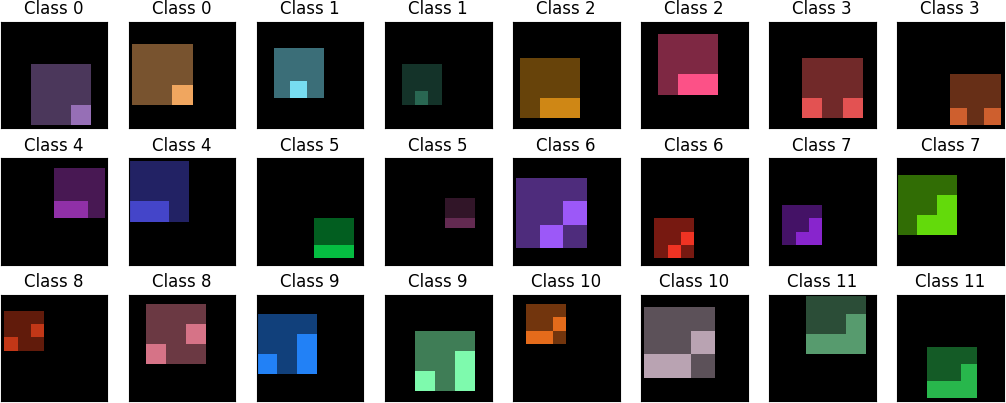
\includegraphics[width=15cm]{blocks}
	\caption{BLOCKS dataset images}
	A sample of synthetic images found in the BLOCKS dataset.
	\label{fig:blocks:1}
\end{figure}

\subsection{\textit{micro}Imagenet} \label{micro-imagenet}
Imagenet\parencite{ilsvr} is a large scale database consisting of over 1 million images of approximately 256x256 pixels in over 20,000 categories. The large size of this dataset makes it appropriate for the training of production models, but is regularly avoided for meta-learning experimentation due to the time required to train on all images. A sub-set of these images were selected to build \textit{mini}Imagenet\parencite{oaamffsl}, which is 60,000 images in 100 classes with 600 images per class. \par
As discussed in section \ref{ml-inputs}, we wish to use this dataset to pre-train the feature extractor of source models, so it is helpful for the training images to be of the same dimensions as those the model will eventually work with. Due to this, we created \textit{micro}Imagenet, which is the same as \textit{mini}Imagenet, but with all of the images scaled to 32x32 pixels to match the dimensions of CIFAR100.

\section{Two-Phase Pre-Training Splits}
As two-phase pre-training requires additional classes to train the body of the source model, we performed the pre-training as according to table \ref{tab:pre-train}.\par
\begin{table}[h!] \label{tab:pre-train}
	\centering
	\begin{tabular}{|l|l|}
		\hline
		\textbf{Meta-learning dataset} & \textbf{Pre-training dataset} \\ \hline
		BLOCKS (classes 1-100)         & BLOCKS (classes 101-139)      \\ \hline
		CIFAR100                       & \textit{microImagenet}        \\ \hline
		Omniglot (classes 1-1000)      & Omniglot (classes 1001-1623)  \\ \hline
	\end{tabular}
	\caption{Datasets/classes used when performing two-phase pre-training}
\end{table}

\section{Hyper-parameters}
The optimiser used for the experiments was Adam (section \ref{adam:1}) as it has proven to yield good results with little effort in finding an appropriate learning rate. A learning rate $5*10^{-4}$ was used for all experiments, as the results of a standard learning-rate finding procedure were inconclusive due to the lengthy time for the loss to begin improving. \par
The number of tunable hyper-parameters were few, with additional parameters being set on a per-experiment basis, as will be discussed later. \par

\section{Software}
The implementation was written using the Python interface for Tensorflow\parencite{tensorflow}, Google's open-source computational framework. Tensorflow has a vast collection of neural network functions pre-written, allows for automatic differentiation, and generally provides a nice environment for deep learning. In addition, Deepmind's Sonnet\parencite{sonnet} was used, which abstracts some of the more complex and verbose aspects of Tensorflow by way of a light wrapper. Graphing and result logging was done using Tensorboard, a visualisation tool included with Tensorflow. \par

\section{Hardware}
As deep-learning is a computationally expensive task, a computer with a high-end modern GPU is required. A computer meeting these specification was provisioned, consisting of two 8GB Nvidia GTX 1080 graphics cards, a quad-core processor and 64GB of memory. The datasets used are relatively small -- collectively consisting of approximately 3.5GB -- so hard-drive space was not a factor that requires consideration.  \par


\chapter{Results} \label{results-chapter}
\section{BLOCKS}
Experimentation began with the BLOCKS dataset, with the expectation that learning a classification model parametrisation is easier on this than the other datasets due to its simpler features. This dataset was designed specifically to be an easier task than any public datasets, thus allowing us to build a proof-of-concept system before employing it on more difficult datasets. \par
We trained a number of Meta-Learner variants on BLOCKS to validate the feasibility of our algorithm and obtained results that indicate successful training. To aide in the stability and speed of training, each experiment was performed using only the source model output head as inputs to the Meta-Learner and used copy-random initialisation. To facilitate this, we utilised two-phase pre-training with the 39 held-out BLOCKS classes. The experiments produced positive results, indicating that the Meta-Learner architecture and algorithm has the capacity to efficiently augment a source model and extend it to a set of previously-unseen classes. \par
Results are reported in table \ref{tab:blocks-scores}, where we present the accuracy, retention and acquisition for these experiments as described in section \ref{metrics}. In addition, the same collection of source models were augmented and trained on the 5-shot task with a standard SGD optimiser to form an upper-bound of performance for naive model augmentation. We trained 50 models with learning rates in the range of $[10^{-5}, 1]$, training for 1 step, and for 5 steps. The highest target score averaged over the 50 models is reported; source score is not reported due to catastrophic forgetting. \\
There are minor variations in retention for the differing model output variants. Acquisition, however, indicates that producing gates and deltas for each parameter best aides the Meta-Learner in target class performance. \par

\begin{table}[h] \label{tab:blocks-scores}
	\centering
	\begin{tabular}{|l|l|l|l|l|l|l|}
		\hline
		\begin{tabular}{@{}l@{}}Meta-Learner \\ Inputs\end{tabular}  & Initialisation & 		\begin{tabular}{@{}l@{}}Meta-Learner \\ Outputs\end{tabular} & \begin{tabular}{@{}l@{}}Source \\ Precision\end{tabular} & \begin{tabular}{@{}l@{}}Target \\ Precision\end{tabular} & Retention      & Acquisition    \\ \hhline{|=|=|=|=|=|=|=|}		
		Naive model & -- & -- & -- & 0.4 & -- & 0.406 \\ \hhline{|=|=|=|=|=|=|=|}
		Head                & Copy-Random    & Deltas               & \textbf{0.712} & 0.668          & \textbf{0.722} & 0.677          \\ \hline
		Head                & Copy-Random    & Gates + Deltas       & 0.708          & \textbf{0.730} & 0.718          & \textbf{0.740} \\ \hline
		Head                & Copy-Random    & Gates + Tanh Deltas  & 0.692          & 0.680          & 0.702          & 0.690          \\ \hline
	\end{tabular}
	\caption{Results of models trained on BLOCKS as defined in section \ref{metrics}; the highest scores in bold.}
\end{table}

These results suggest that while the outputs certainly do affect the performance of the target model, retention appears to be much more stable than acquisition. Retention measure's the ability of a model to retain the classification accuracy of the source classes, and therefore reflects what is in itself a more stable task, as the Meta-Learner must essentially act as a modified auto-encoder where ideal performance is to learn a 1-to-1 mapping from inputs to outputs. Acquisition is a less stable task, as it requires that the Meta-Learner adequately applies the gradients given as inputs to learn to classify between unseen classes, which is more difficult. \par
It is worth noting that there appears to be a trade-off between retention and acquisition, and with these results indicating success, we move to the public dataset Omniglot in hopes of replicating the performance, and to further explore this trade-off.


\section{Omniglot}
The Omniglot\parencite{omniglot} public dataset was the main focus of experimentation, as it is an easier task than CIFAR100, but is recognised throughout the meta-learning community as a dataset representative of real computer-vision tasks. The visual features found in Omniglot are sufficiently complex to be challenging -- especially when contrasted with BLOCKS, due to the addition of rounded edges and arbitrarily-angled lines among others. \par
We first applied the same Meta-Learner variant to this dataset, passing the source model head as inputs, using copy-random initialisation, and with the Meta-Learner producing a gate and a delta per weight. This yielded promising results, with retention and acquisition both indicating success (table \ref{tab:omniglot-results}). As with BLOCKS, we perform the same naive model augmentation on Omniglot. Our solution performs substantially better than the naive solution, indicating that the Meta-Learner leverages additional information due to the episodic meta learning training environment. With successful results indicated on this dataset, we explore Meta-Learner variants and their effects on performance. \par

\subsection{Meta-Learner Inputs}
We begin our experiments by determining the inputs to the model that provide the best results, to serve as the standard inputs for the remainder of experimentation. As shown in table \ref{tab:omniglot-results}, switching from passing only the source model head as inputs to passing the source model body and head significantly improves performance, which is most pronounced in the retention, where there is an increase of $0.8$. This allows the Meta-Learner to not only gain a larger view of the source model, but also to re-parametrise the body of the model, allowing for the adjustment of feature-extractors as necessary; conversely, passing only the head of the model enforces a fixed feature extractor. We therefore give the entire source model as inputs to the Meta-Learner for the remainder of our experiments. 

\subsection{Meta-Learner Outputs}
\subsubsection{Deltas}
In its most basic form, the Meta-Learner can act as a replacement for a standard optimizer, simply updating the weights by adding a delta as shown in equation \ref{eqn-delta-updates}. Table \ref{tab:omniglot-results} shows that this gives sub-par performance when compared to the variant with the ability to gate existing weights. \par
For the target model output layer, we plotted the scale of the produced deltas with respect to the pre-existing weights to gain some understanding of how the two components interact (figure \ref{fig:deltascale:1}). A score of 1 indicates that the average magnitude of the deltas is equal to that of the existing weights, and a score of 2 indicates that it is twice as large. Equation \ref{delta-rule} shows this calculation for source weights/deltas; it is similarly calculated for target weights/deltas.
\begin{align} \label{delta-rule}
\ddfrac{\frac{1}{n}\sum_{i=1}^{n}|\Delta_{M_{S,i}}|}{\frac{1}{n}\sum_{i=1}^{n}|\theta_{S,i}|}
\end{align}
Interestingly, the deltas far outweigh the scale of the weights -- by an order of magnitude. It would be reasonable to expect that the deltas are in the same order of magnitude as the weights, as this would allow for some of the pre-existing weights to simply be ``passed-through'' unchanged as required. There appears to be no difference in scale between either the deltas that correspond to the source class output weights and those that correspond to the target class output weights. This means that the Meta-Learner is effectively disregarding the existing weights and producing a new set of weights, as the sheer magnitude of the deltas would far outweigh any contribution from the pre-existing weights.

\begin{figure}[h!]
	\centering
	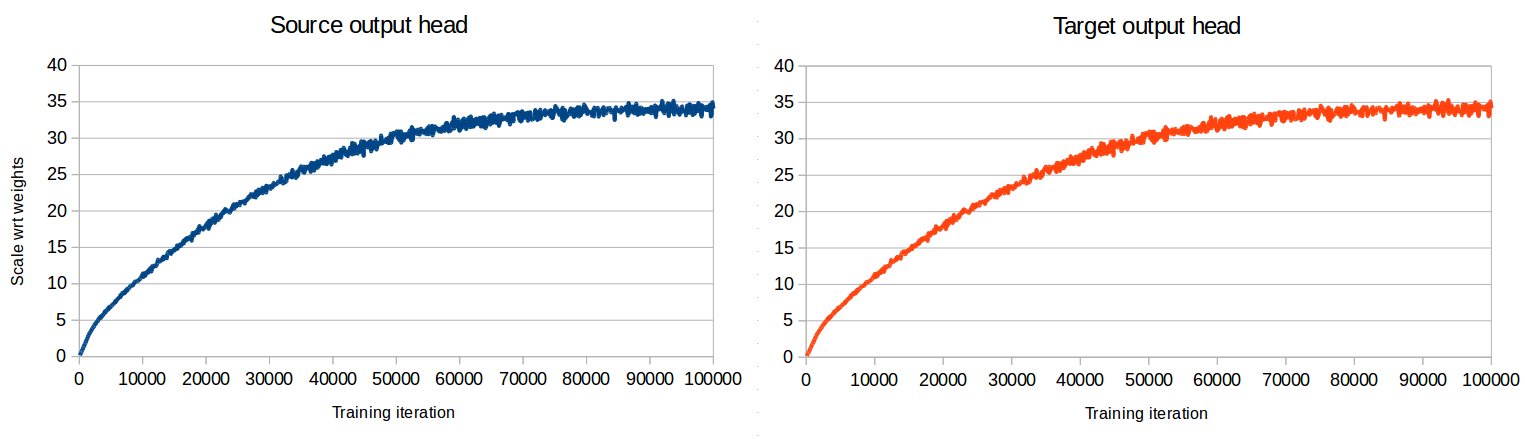
\includegraphics[width=16cm]{deltascale}
	\caption{Delta scales}
	The scale of the produced deltas with respect to the corresponding weights as detailed in equation \ref{delta-rule}.
	\label{fig:deltascale:1}
\end{figure}

\subsubsection{Gates and Deltas}
As the Meta-Learner is thus far effectively ignoring the pre-existing weights, we aimed to give it the means to selectively keep or delete them, by producing a per-weight gate value in $[0, 1]$. To monitor the Meta-Learner's usage of these gates, we plot the distribution of gate values for the source and target class output heads separately over time. Figure \ref{fig:gate-distrib:1} shows these gate distributions for each of the initialisation schemes. \par
The gates tend to be less than 0.5 for both the source and target classes, indicating that the Meta-Learner doesn't find much benefit in retaining the existing weight values. This is to be expected for the target classes with random and copy-random initialisation, however, the gates follow the same distribution for the source-classes as well. We infer that the model doesn't clearly distinguish between source and target classes in its weight generation, and instead largely discards all existing weight values. For the case of copy initialisation, the gates remain closer to 0.5 which indicates that the Meta-Learner does utilise the existing weights. \par

\begin{figure}[!h]
	\centering
	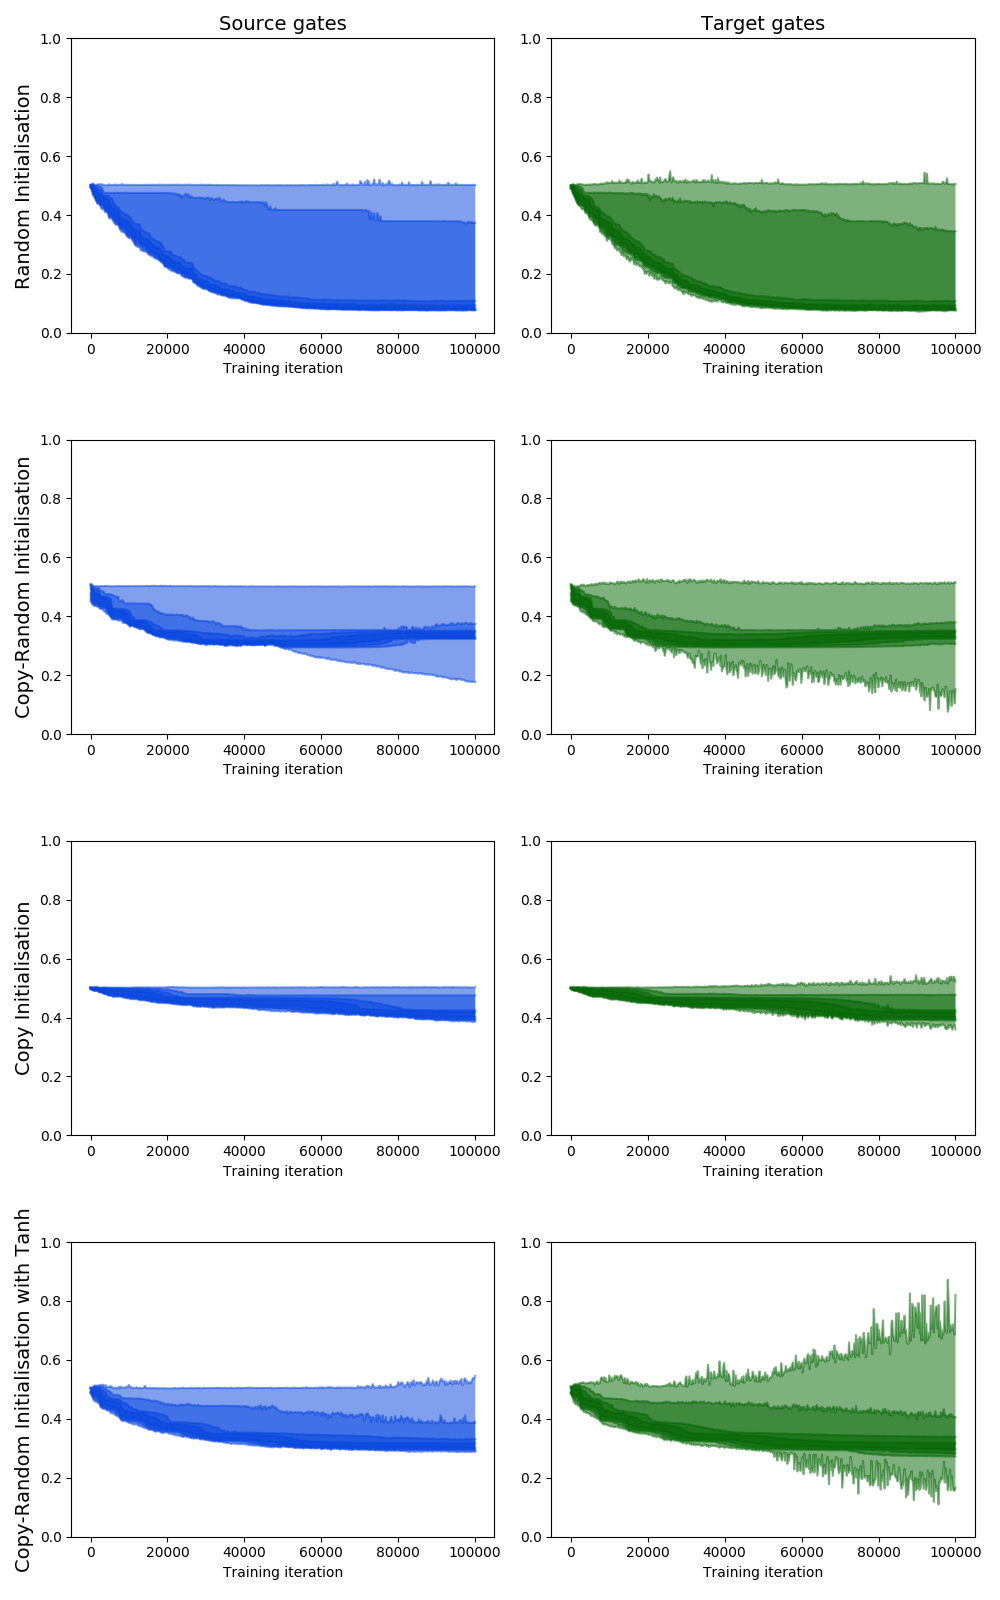
\includegraphics[width=14cm]{gate-distrib}
	\caption{Distribution of gate values for the output heads}
	Gates are separated into source and target classes. Values from 0 to 1 indicates the Meta-Learner's inclination to forget or retain existing weights.
	\label{fig:gate-distrib:1}
\end{figure}

\subsubsection{Gates and Tanh Deltas}
The large scale of produced deltas and the Meta-Learner's inclination to zero-out existing weights suggests that the majority of the source model is being discarded. This requires that the Meta-Learner must not only learn how to produce good deltas, but also reproduce the existing internal representation found in the source model. We aimed to disallow this outweighing of the source model by applying a tanh layer to the produced deltas. The tanh function is effectively a rescaled sigmoid function, which squishes values into the range $[-1, 1]$ -- thereby forcing the magnitude of the deltas to never exceed 1. \par
We observed that this restriction on delta magnitude led to better utilisation of source model weights (figure \ref{fig:gate-distrib:1}, bottom), but also to a degradation of performance -- especially with the source classes (table \ref{tab:omniglot-results}). In addition, the gates relating to the target classes stayed nearer to 0.5, with a much larger variance than previously observed. We infer that as Meta-Learner does not learn a clear distinction between weights relating to the source classes and those relating to the target classes, it therefore is incapable of adequately retaining weights of importance while masking out those less useful. This results in the deletion of important knowledge pertaining to the source head, and therefore a deterioration of source class performance.

\subsection{Weight Initialisation}
\subsubsection{Random Initialisation}
The initialisation of the weights in the target class output head is critical, and as such, we explored three weight initialisation schemes. Random initialisation -- while commonplace in traditional deep learning -- leads to a degradation in performance for our task. Initialisation in this manner introduces a stochastic element to the inputs, as the Meta-Learner will be given different inputs (albeit from the same distribution) every time, resulting in gates tending towards zero to negate this source of noise. \par
As the Meta-Learner has difficulty distinguishing source class weights from target class weights, it learns an aggressive gating strategy to ignore the introduced noise and discards important source class knowledge embedded in the existing weights. This is reflected in figure \ref{fig:gate-distrib:1}, where the gates for both source and targets both have a mean value close to zero. This is also shown in table \ref{tab:omniglot-results}, where the source class performance is poor.

\subsubsection{Copy-Random Initialisation}
To remove the stochasticity in target weight initialisation, we introduce copy-random initialisation. By sampling the target class output weights only once and repeatedly using them for each model initialisation, the Meta-Learner does not need to counteract the introduction of newly-sampled random inputs for each episode. Our results indicate that this does in fact aid performance on the source classes over random initialisation. The results in table \ref{tab:omniglot-results} indicate that this boost in source class performance does come with a decrease in target class performance, though this is margin, so copy-random initialisation is used as the default initialisation for experiments when varying other aspects.

\subsubsection{Copy Initialisation}
We copy weights from the source class output head into the target class output head as described in section \ref{weight-init}. This yields surprising results, as it achieves the highest average score of all variants (\ref{tab:omniglot-results}). We infer that it works well on Omniglot due to the generality of features found in the dataset. As all classes in Omniglot are handwritten characters, the features they are composed of are not only simplistic, but transferable. The domain is very narrow, and therefore the characteristics of edges, lines, curves etc. are similar across its entirety. This allows a neural network to take advantage by sharing these general features across classes. \par
If we consider the features found in a neural network trained on CIFAR100 (which has classes as varied as ``bus'' and ``dolphin'') the model typically extracts high-level features such as wheels and eyes\parencite{deepvis}. Therefore the output layer of a neural network -- which performs the mapping between these features and classes -- will have large positive weights mapping $wheel\rightarrow bus$ and $eye\rightarrow dolphin$, and large negative weights mapping $eye\rightarrow bus$ and $wheel\rightarrow dolphin$. With a copy initialisation scheme for a varied dataset such as this, the Meta-Learner would essentially need to ``undo'' this in order to re-map to the new target classes. A model for a narrow-domain dataset such as Omniglot would not have such disparity in feature importance between classes, and therefore requires less work to re-map effectively. \par
Our results suggest that for Omniglot, copy initialisation acts somewhat as a form of pre-training much like transfer learning. However, we expect that this initialisation scheme would not be as effective as copy-random initialisation on a larger-domain dataset.


\begin{table}[h!] 
	\centering
	\begin{tabular}{|l|l|l|l|l|l|l|}
		\hline
		\begin{tabular}{@{}l@{}}Meta-Learner \\ Inputs\end{tabular}  & Initialisation & 		\begin{tabular}{@{}l@{}}Meta-Learner \\ Outputs\end{tabular} & \begin{tabular}{@{}l@{}}Source \\ Precision\end{tabular} & \begin{tabular}{@{}l@{}}Target \\ Precision\end{tabular} & Retention      & Acquisition    \\ \hhline{|=|=|=|=|=|=|=|}
		Naive model & -- & -- & -- & 0.292 & -- & 0.373 \\ \hhline{|=|=|=|=|=|=|=|}
		Head        & Copy-Random & Gates + Deltas      & 0.619          & 0.802          & 0.790          & 1.023          \\ \hline
		Body + Head & Copy-Random & Gates + Deltas      & 0.692          & 0.832          & 0.883          & 1.062          \\ \hline
		Body + Head & Copy-Random & Deltas              & 0.613          & 0.646          & 0.783          & 0.825          \\ \hline
		Body + Head & Copy-Random & Gates + Tanh Deltas & 0.582          & 0.718          & 0.743          & 0.916          \\ \hline
		Body + Head & Copy        & Gates + Deltas      & \textbf{0.693} & 0.835          & \textbf{0.885} & 1.065          \\ \hline
		Body + Head & Rand        & Gates + Deltas      & 0.586          & \textbf{0.863} & 0.748          & \textbf{1.101} \\ \hline
	\end{tabular}
	\caption{Results of models trained on Omniglot as defined in section \ref{metrics}; the highest scores in bold.}
	\label{tab:omniglot-results}
\end{table}

\section{CIFAR100}
Applying the Meta-Learner to the task of model augmentation using CIFAR100 proved to be a difficult task, and yielded poor results. A recurring problem was prediction exclusivity, where the Meta-Learner ``gets stuck'' producing target models that are only able to provide predictions for either the source classes \textit{or} the target classes. Figure \ref{fig:cifaraccuracy:1} demonstrates this effect by showing the accuracy on the source and target datasets for a number of Meta-Learner variants. As a means of measuring this class exclusivity, we devised the metric \textit{Batch Prediction Entropy}. \par
\begin{figure}[!h!]
	\centering
	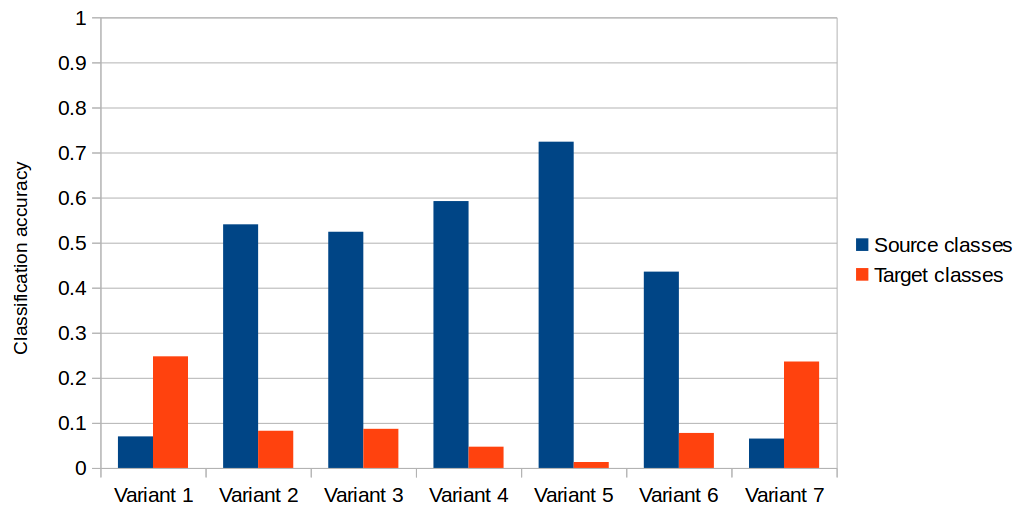
\includegraphics[width=13cm]{cifaraccuracy}
	\caption{Summed batch prediction scores}
	Comparison of source/target classification accuracy on CIFAR100
	\label{fig:cifaraccuracy:1}
\end{figure}

\subsubsection{Batch Prediction Entropy}
In the context of information theory, entropy is a measure of the rate of information produced by a data source. Its general formula is given below, where we have chosen to use the natural logarithm:
\begin{align}
H(X) &= \sum_{i=1}^{n}P(x_i) log(P(x_i)) \label{entropyfunc}
\end{align}

It is typically desired that the entropy of a predictor is large, as this means that the system is producing a large amount of information with each prediction -- corresponding to high-confidence predictions. However, considering an entire batch of predictions, if we are to sum the raw outputs from each example into a single discrete probability distribution as shown in figure \ref{fig:totalbatchpredscores:1}, we would hope that each class has a similar total magnitude (assuming the batch contains an identical number of elements per class); a difference in magnitude indicates a disparity in class predictions. We therefore developed Batch Prediction Entropy (BPE) to give a quantitative measure of class prediction disparity, and to provide an indicator of class exclusivity. BPE is calculated as the entropy of the sum of the raw predictions of an entire batch of examples. 

\begin{figure}[h!]
	\centering
	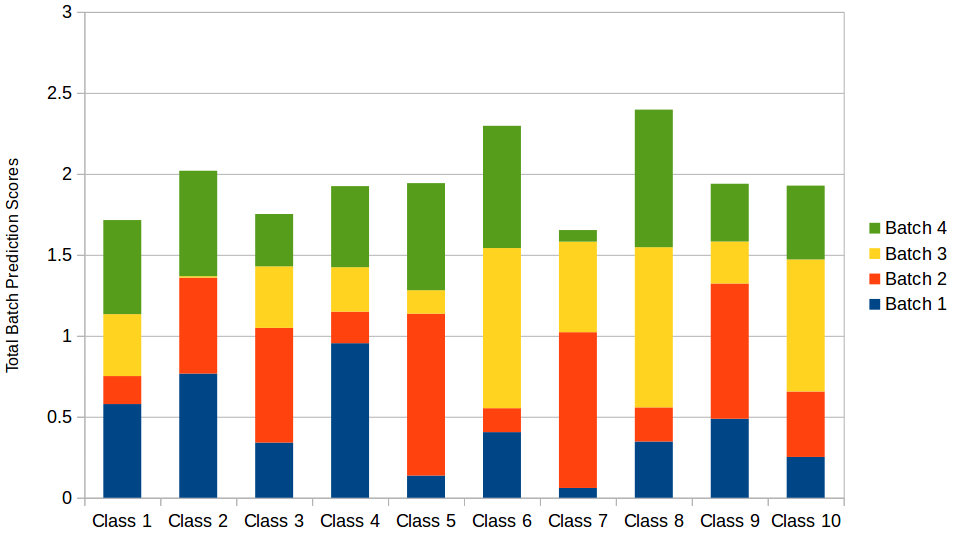
\includegraphics[width=13cm]{totalbatchpredscores}
	\caption{Example summed raw prediction values}
	The sum of raw prediction values across an entire batch should ideally be of similar magnitudes
	\label{fig:totalbatchpredscores:1}
\end{figure}

We first construct a $B{\times}N$ matrix $\bm{\hat{Y}}$, where $B$ is the batch size, $N$ is the number of classes, and element $\hat{y}_{ik}$ is the raw predicted probability for class $k$ in batch element $i$:
\begin{align} \label{eq:bpe:1}
\bm{\hat{Y}} = \begin{bmatrix}
\hat{y}_{11} & \hat{y}_{12} & \hat{y}_{13} & \dots  & \hat{y}_{1N} \\
\hat{y}_{21} & \hat{y}_{22} & \hat{y}_{23} & \dots  & \hat{y}_{2N} \\
\vdots & \vdots & \vdots & \ddots & \vdots \\
\hat{y}_{B1} & \hat{y}_{B2} & \hat{y}_{B3} & \dots  & \hat{y}_{BN}
\end{bmatrix}
\end{align}
We then sum over the columns to produce the total batch prediction scores:
\begin{align} \label{eq:bpe:2}
\bm{\tilde{y}} &= (1, 1, \dots, 1)\bm{\hat{Y}} \\
  &= \big(\hat{y}_{11} + \hat{y}_{21} + \dots + \hat{y}_{B1}, \dots, \hat{y}_{1N} + \hat{y}_{2N} + \dots + \hat{y}_{BN}\big)
\end{align}
The Batch Prediction Entropy is then the entropy as given in equation \ref{entropyfunc} of this resultant vector:
\begin{align}
BPE(\bm{\hat{Y}}) = H(\bm{\tilde{y}})
\end{align}
This metric gives us a quantitative measure of entropy over an entire batch of predictions. Unlike for a single example -- where we desire that entropy is high -- it is desired that the BPE of a model is low, corresponding to a similar level of prediction confidence among all classes. A low BPE is an indicator of minimal disparity between class prediction frequency (how often each class is predicted) and class prediction confidence (the confidence with which each class is predicted). \par
BPE is also useful as a means of detecting dying neurons -- a relatively common failure in neural networks where neurons reach the value of zero and never recover. This is typically the result of an incorrect learning rate/optimiser configuration, or a complex network with gradients failing to give strong-enough signal to train correctly. Dying neurons effectively shrink the model capacity, and when occurring in the final layer can cause the model to ``get stuck'' predicting the same classes. \par

With this metric in place, we trained our model on the CIFAR100 dataset, monitoring BPE to assess the model's capability; some results are shown in figure \ref{fig:totalbatchpredgraph:1} for two implementations. Although the results of only two implementations are given, these are indicative of the results for every implementation. In figure \ref{fig:totalbatchpredgraph:1}a, we see that the model only learns to predict the source classes, and in figure \ref{fig:totalbatchpredgraph:1}b the model only learns to predict the target classes. Each implementation produced the same result, with the model favouring one set of classes over the other. In contrast, the BPE while training the BLOCKS dataset (figure \ref{fig:totalbatchpredgraphblocks:1}) had a downward trend for both the source and target classes, indicating that the model was learning a balanced prediction distribution across output classes. \par
\begin{figure}[h!]
	\centering
	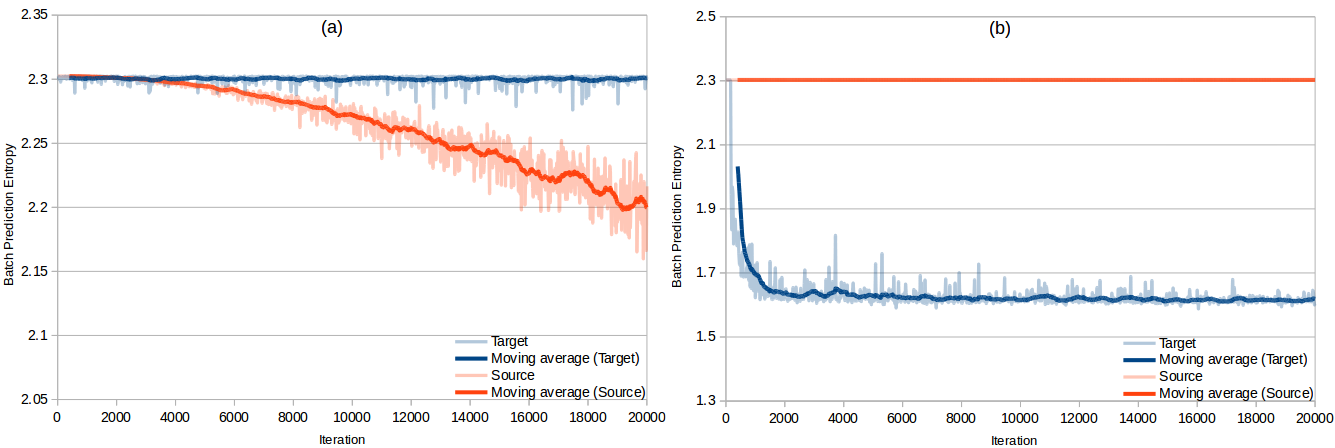
\includegraphics[width=17.5cm]{totalbatchpredgraph}
	\caption{CIFAR100 Batch Prediction Entropy}
	BPE of two implementations for the CIFAR100 task. The model begins learning to predict either the source or target classes exclusively in (a) and (b), respectively.
	\label{fig:totalbatchpredgraph:1}
\end{figure}

\begin{figure}[h!]
	\centering
	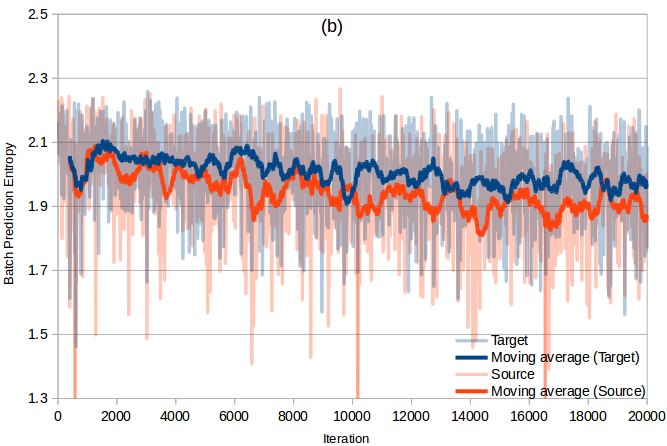
\includegraphics[width=10cm]{totalbatchpredgraphblocks}
	\caption{BLOCKS Batch Prediction Entropy}
	BPE for the BLOCKS task. A consistent decrease in BPE indicates that a model is learning evenly across all classes.
	\label{fig:totalbatchpredgraphblocks:1}
\end{figure}

We hypothesise that the features in the CIFAR100 dataset are too complex for our implementation, and it therefore cannot adequately learn the relationships between the parameters of a model trained for this task. The same results were produced when performing the simpler task described in section \ref{ml-inputs}, where only the head of the model is given as input to the Meta-Learner. \par
For this, we performed two-phase pre-training as described in section \ref{pre-training}, pre-training the body of the source models on microImagenet, and fine-tuning each head with the CIFAR100 source classes. Despite the increased simplicity of this experiment, the same results were produced, with the model failing to correctly classify between both sets of classes. \par


\section{Discussion}
Our comparison to the naive solution on Omniglot indicates that our most-successful technique -- with an acquisition of 0.875 -- is $\sim$3x as effective at adapting to new classes from few examples as a non-meta-learning technique. The highest acquisition of 1.101 also demonstrates that our Meta-Learner is a very efficient learner, as it can generate model parameters in a single pass that perform $\sim$10\% better than the source model. \par
We also compare performance to the 5-shot meta-learning techniques discussed in chapter \ref{related:1}, and find that when compared the best-performer on Omniglot (MAML\parencite{maml}), our model is 83.54\% as effective at adapting to new classes. We do however, have the added constraint that we must remain performant on the source classes -- a restriction that MAML does not need to adhere to. While not performing with such success as specific few-shot meta-learning systems, our solution performs very well for being combined with the additional task of continuous learning. \par


\chapter{Conclusion}
The task of few-shot continuous learning is inherently challenging, and is still -- as of yet -- unsolved. No prior research for this specific task was encountered throughout the research period, though some works come close. We have therefore investigated the effects of catastrophic forgetting in the context of image-classification neural networks, and developed a novel solution for the problem. We additionally explored how a convolutional neural network can be applied optimisation-based few-shot learning. \par
Our experimentation shows that a convolutional neural network is capable of re-parametrising a neural network, and that local weight/gradient information is sufficient to do so. This represents a step forward in the realm of learnt optimisation, indicating that a temporal network such as an RNN is not required to perform weight updates, as a single optimisation step with only locally-aggregated information can sufficiently improve model performance. We also show that the type of update rule used (deltas, gates, etc.) has a significant impact on model optimisation, illustrating that there is work to be done in the development of optimisers of neural networks, be it meta learning or otherwise. Time constraints limited our variants to a select subset of those we deemed worthy of exploration, and therefore leave some additional variants to future works.

\section{Future works} \label{future-works}
\subsubsection{Architecture Invariance}
There were several design decisions made throughout the development of the Meta-Learner that tie it to the source-model architecture of a fully-convolutional neural network without biases. A future iteration of this solution would allow for complete architecture invariance, permitting the augmentation of models with fully-connected layers, and with biases added to the layers. \par
As the Meta-Learner performs embedding and unembedding as part of its procedure, the support of these model features would require only that an embedding function is designed. The Meta-Learner already learns adequate embedding techniques, and the extension of these to additional inputs is relatively trivial. Our research does not show whether a Meta-Learner trained on one architecture would be truly invariant to changes in architecture, but training on a diverse collection of architectures would mitigate this.

\subsubsection{Split-Steam Encoder}
As we found that the Meta-Learner had difficulty distinguishing between source-class weights and target-class weights, future work would be to adapt the structure of the encoder-decoder to enforce their separation. A basic overview of some possible options is given in figure \ref{fig:split-stream:1}, where the source and target class head weights/gradients are separated from the body. Performing the operation in this manner would allow for the Meta-Learner to encode them separately, giving an opportunity to learn a different internal representation in order to produce sufficiently-varied gate values.

\begin{figure}[!h]
	\centering
	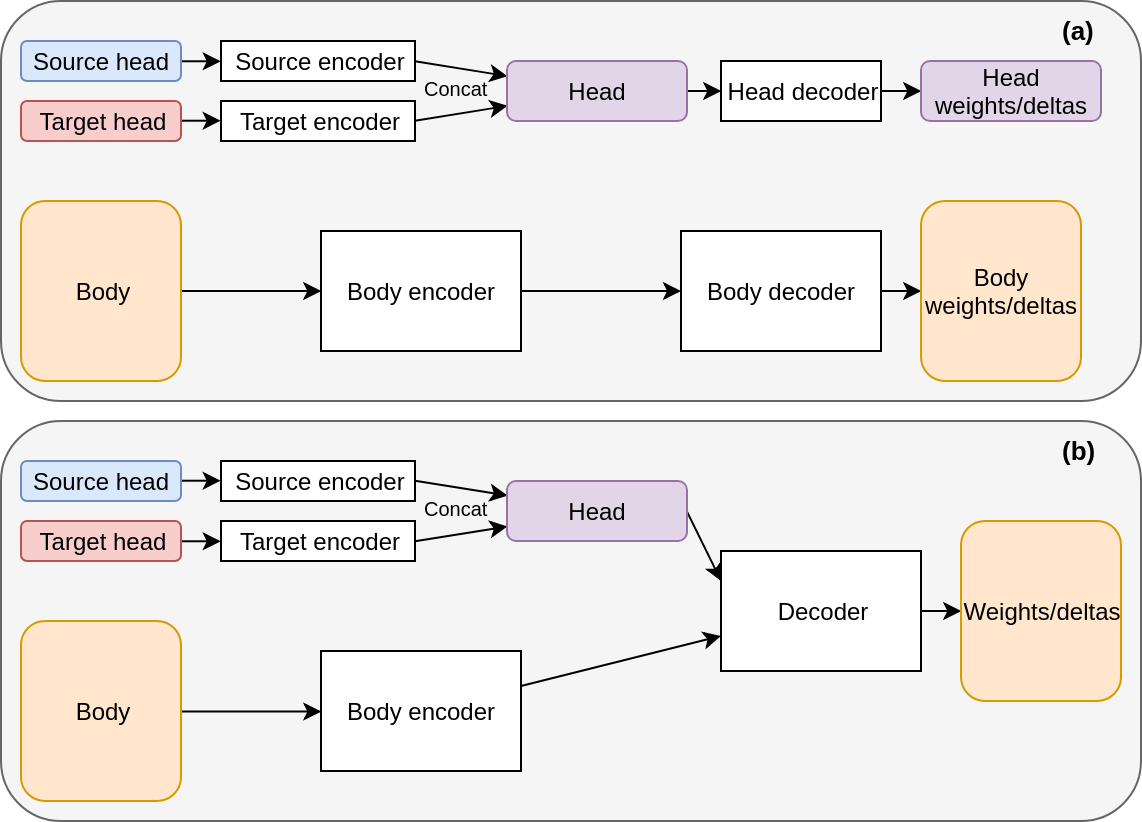
\includegraphics[width=13cm]{split-stream}
	\caption{Possible split-stream encoder architectures}
	\label{fig:split-stream:1}
	A split-stream encoder could separate the source and target head weights/gradients from the body weights/gradients, encode and decode them separately (a). The encodings could alternatively be decoded all together (b).
\end{figure}




\printbibliography




\end{document}
